\section{Balance of mass for an open system}
\label{sect2} The body of interest, $\sB$, occupies the open
region $\Omega_0\subset\mathbb{R}^3$ in the reference
configuration. Points in $\sB$ are parameterized by their
reference positions, $\bX$. The deformation of $\sB$ is a
point-to-point map, $\Bvarphi (\bX,t)\in\mathbb{R}^3$, of
$\Omega_0$, carrying the point at $\bX$ to its current position
$\bx = \Bvarphi(\bX,t)$, at time $t\in [0,T]$. In its current
configuration, $\sB$ occupies the open region $\Omega_t =
\Bvarphi_t(\Omega_0),\; \Omega_t\subset\mathbb{R}^3$ (see Figure
\ref{potato}). The tangent map of $\Bvarphi$ is the deformation
gradient $\bF :=
\partial\Bvarphi/\partial\bX$.
\begin{figure}[ht]
\centering\psfrag{BIGX}{\small$\bX$} \psfrag{SMX}{\small$\bx$}
\psfrag{PI}{\small$\Pi^\mathrm{\iota}$}
\psfrag{PPI}{\small$\pi^\mathrm{\iota}$}
\psfrag{MN}{\small$\bN\cdot\bM^{\iota}$}
\psfrag{MMN}{\small$\bn\cdot\bm^\mathrm{\iota}$}
\psfrag{SN}{\small$\bP\bN$} \psfrag{SSN}{\small$\Bsigma\bn$}
\psfrag{PHI}{\small$\Bvarphi$} \psfrag{WO}{\small$\Omega_0$}
\psfrag{WT}{\small$\Omega_t$}
{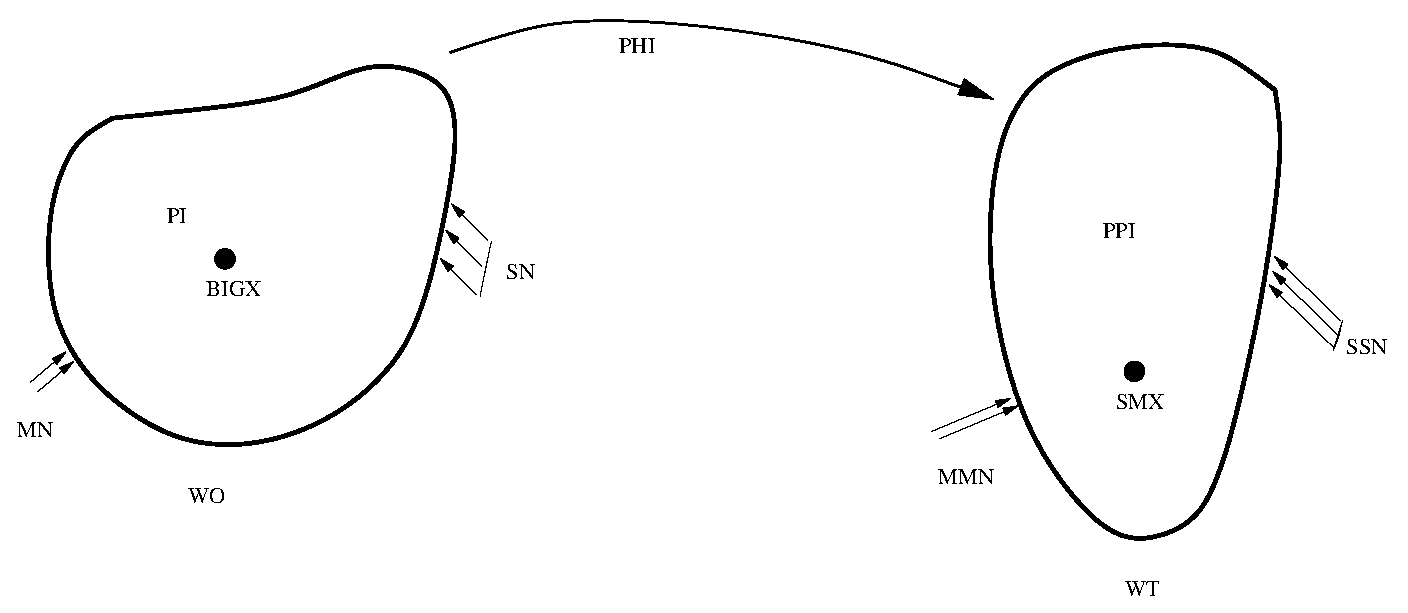
\includegraphics[width=14cm]{images/growth1.eps}} \caption{The continuum
body with diffusing species and under stress.}\label{potato}
\end{figure}

The body consists of several species, of which the solid phase of
the tissue is denoted $\mathrm{s}$, and the fluid phase is
$\mathrm{f}$. The remaining species, $\alpha,\dots,\omega$, are
precursors of the tissue or byproducts of its breakdown in
chemical reactions. The index $\iota$ will be used to indicate an
arbitrary species. (Where appropriate, we will use the term
``system'' to refer to the species collectively. Where the
presence of several species is an unimportant fact, we will use
the term ``body''. ) The system is open with respect to mass.
Species $\alpha,\dots,\omega$ have sources/sinks,
$\Pi^\alpha,\dots,\Pi^\omega$, and mass fluxes,
$\bM^\alpha,\dots,\bM^\omega$, respectively. The sources specify
mass production rates per unit volume of the body in its reference
configuration, $\Omega_0$. The fluxes specify mass flow rates per
unit cross-sectional area in $\Omega_0$. Importantly, \emph{these
flux vectors are defined relative to the solid phase}. As
discussed in Section \ref{sect1}, the solid tissue phase has only
a mass source/sink associated with it, and no flux. The fluid
tissue phase has only a mass flux, and no
source/sink\footnote{Considering the case of the lymphatic fluid,
this implies that lymph glands are assumed not to be present.}.

Since the solid phase, $\mathrm{s}$, does not undergo transport,
its motion is specified entirely by $\Bvarphi(\bX,t)$. We describe
the remaining species $\mathrm{f},\alpha,\dots,\omega$ as
convecting with the solid phase and diffusing with respect to it.
They therefore have a velocity relative to $\mathrm{s}$. Since the
remaining species convect with $\mathrm{s}$, it implies a local
homogenization of deformation. The modelling assumption is made
that at each point, $\bX$, the individual phases undergo the same
deformation.

We define concentrations of the species
$\rho_0^\iota=\bar{\rho}_0^\iota f^\iota$ as masses per unit
volume in $\Omega_0$. The intrinsic species density is
$\bar{\rho}_0^\iota$, and $f^\iota$ is the volume fraction of
$\iota$, for $\iota = \mathrm{s,f},\alpha,\dots,\omega$. In an
experiment it is far easier to measure the concentration,
$\rho_0^\iota$, rather than the intrinsic species density,
$\bar{\rho}_0^\iota$\footnote{In our experiments we have measured
the mass concentration $\rho_0^\iota$ of collagen in engineered
tendons grown \emph{in vitro}. These results will be presented
elsewhere \citep{Calve:04}.}. The concentrations also have
the property $\sum\limits_{\iota}\rho_0^\iota = \rho_0$, the total
material density of the tissue, with the sum being over all
species $\mathrm{s,f},\alpha,\dots,\omega$. The concentrations,
$\rho_0^\iota$, change as a result of mass transport and
inter-conversion of species, implying that the total density in
the reference configuration, $\rho_0$, changes with time. They are
parameterized as $\rho_0^\iota(\bX,t)$.



\subsection{Balance of mass in the reference configuration}
\label{sect2.1} Recall that $\Omega_0$ is a fixed volume. The
statement of balance of mass of the solid phase of the tissue,
written in integral form over $\Omega_0$, is

\begin{equation}
\frac{\mathrm{d}}{\mathrm{d}t} \int\limits_{\Omega_0}
\rho_0^\mathrm{s} (\bX,t)\mathrm{d}V = \int\limits_{\Omega_0}
\Pi^\mathrm{s} (\bX,t)\mathrm{d}V. \label{massbalintA}
\end{equation}

\noindent Since the solid phase of the tissue does not undergo
mass transport, there is no associated flux. Localizing the result
gives

\begin{equation}
\frac{\partial\rho_0^\mathrm{s}}{\partial t} = \Pi^\mathrm{s},
\label{massballocA}
\end{equation}
\noindent where the explicit dependence upon position and time has
been suppressed.

The fluid phase of the tissue, $\mathrm{f}$, may be thought of as
the interstitial or lymphatic fluid that perfuses the tissue. As
explained above, we do not consider sources of fluid in the region
of interest. The fluid therefore enters and leaves $\Omega_0$ as a
flux, $\bM^\mathrm{f}$. The balance of mass in integral form is
\begin{equation}
\frac{\mathrm{d}}{\mathrm{d}t} \int\limits_{\Omega_0}
\rho_0^\mathrm{f} (\bX,t)\mathrm{d}V =
-\int_{\partial\Omega_0}\bM^\mathrm{f}(\bX,t)\cdot\bN \mathrm{d}A,
\label{massbalintB}
\end{equation}

\noindent where $\bN$ is the unit outward normal to the boundary,
$\partial\Omega_0$. Applying the Divergence Theorem to the surface
integral and localizing the result gives
\begin{equation}
\frac{\partial\rho_0^\mathrm{f}}{\partial t} = -
\Bnabla\cdot\bM^\mathrm{f}, \label{massballocB}
\end{equation}

\noindent where $\Bnabla(\bullet)$ is the gradient operator
defined on $\Omega_0$, and $\Bnabla\cdot(\bullet)$ denotes the
divergence of a vector or tensor argument on $\Omega_0$.

For the precursor and byproduct species,
$\iota=\alpha,\dots,\omega$, the balance of mass in integral form
is
\begin{equation}
\frac{\mathrm{d}}{\mathrm{d}t} \int\limits_{\Omega_0} \rho_0^\iota
(\bX,t)\mathrm{d}V = \int\limits_{\Omega_0} \Pi^\iota
(\bX,t)\mathrm{d}V
-\int_{\partial\Omega_0}\bM^\iota(\bX,t)\cdot\bN \mathrm{d}A.
\label{massbalintI}
\end{equation}

\noindent In local form it is
\begin{equation}
\frac{\partial\rho_0^\iota}{\partial t} = \Pi^\iota -
\Bnabla\cdot\bM^\iota,\;\forall\,\iota=\alpha,\dots,\omega.
\label{massballocI}
\end{equation}

\noindent Of course, this last equation is the general form of
mass balance for any species $\iota$, recalling that in
particular, $\bM^\mathrm{s} = \bzero$ and $\Pi^\mathrm{f} = 0$.
This form will be used in the development that follows.

The fluxes,
$\bM^\iota,\;\forall\,\iota=\mathrm{f},\alpha,\dots,\omega$,
represent mass transport of the fluid, of precursors to the
reaction site, and of byproducts from sites of tissue breakdown.
The sources,
$\Pi^\iota,\;\forall\iota=\mathrm{s},\alpha,\dots,\omega$, arise
from inter-conversion of species. The sources/sinks in
(\ref{massballocA}) and (\ref{massballocI}) are therefore related,
as tissue and byproducts are formed by consuming precursors (amino
acids and nutrients, for instance). To maintain a degree of
simplicity in this initial exposition, we will restrict our
description of tissue breakdown to the reverse of this reaction.

The sources, $\Pi^\iota$ for various species, satisfy a relation
that is arrived as follows: Summing (\ref{massballocI}) over all
species leads to the law of mass balance for the system,
\begin{equation}
\sum\limits_\iota\frac{\partial\rho_0^\iota}{\partial t} =
\sum\limits_\iota\left(\Pi^\iota - \Bnabla\cdot\bM^\iota\right),
\label{massballocItot}
\end{equation}

\noindent where the sum runs over all species, with
$\Pi^\mathrm{f} = 0$ and $\bM^\mathrm{s} = \bzero$. Alternatively,
in writing the mass balance equation for the system, the
interconversion terms (sources/sinks) play no role, and only the
fluxes at the boundaries need be accounted for. In integral form
we have
\begin{displaymath}
\frac{\mathrm{d}}{\mathrm{d}t}\sum\limits_\iota\int\limits_{\Omega_0}\rho_0^\iota
\mathrm{d}V =
-\sum\limits_\iota\int\limits_{\partial\Omega_0}\bM^\iota\cdot\bN
\mathrm{d}A.
\end{displaymath}

\noindent Applying the Divergence Theorem and localizing leads to
\begin{equation}
\sum\limits_\iota \frac{\partial\rho_0^\iota}{\partial t} =
\sum\limits_\iota(-\Bnabla\bM^\iota). \label{massballoctot}
\end{equation}

\noindent Comparing the equivalent forms (\ref{massballocItot})
and (\ref{massballoctot}) it emerges that the sources and sinks
satisfy
\begin{equation}
\sum\limits_\iota\Pi^\iota = 0, \label{sourcebalance}
\end{equation}

\noindent a conclusion that is consistent with classical mixture
theory \citep{TruesdellNoll:65}. The section that follows contains
an example in which the Law of Mass Action is invoked to describe
a set of inter-related sources, $\Pi^\iota$.

\subsubsection{Sources, sinks and stoichiometry: An example based upon the Law of Mass Action}\label{sect2.1.1}

The conversion of precursors to tissue and the reverse process of
its breakdown are governed by a series of chemical reactions. The
stoichiometry of these reactions varies in a limited range.
Continuing in the simple vein adopted above, it is assumed that
the formation of tissue and byproducts from precursors, and the
breakdown of tissue, are governed by the forward and reverse
directions of a single reaction:
\begin{equation}
\sum\limits_{\iota=\alpha}^{\omega} n_\iota[\iota] \longrightarrow
[\mathrm{s}]. \label{chemreac}
\end{equation}

\noindent Here, $n_\iota$ is the (possibly fractional) number of
moles of species $\iota$ in the reaction. For a tissue precursor,
$n_\iota > 0$, and for a byproduct, $n_\iota < 0$. By the Law of
Mass Action for this reaction, the rate of the forward reaction
(number of moles of $\mathrm{s}$ produced per unit time, per unit
volume in $\Omega_0$) is
$k_\mathrm{f}\prod\limits_{\iota=\alpha}^\omega
[\rho_0^\iota]^{n_\iota}$, where $\prod$ on the right hand-side
denotes a product, not to be confused with the source, $\Pi$. The
rate of the reverse reaction (number of moles of $\mathrm{s}$
consumed per unit time, per unit volume in $\Omega_0$) is
$k_\mathrm{r}[\rho_0^\mathrm{s}]$, where $k_f$ and $k_r$ are the
corresponding reaction rates. Assuming, for the purpose of this
example, that the solid phase is a single compound, let the
molecular weight of $\mathrm{s}$ be $\sM_\mathrm{s}$. From the
above arguments the source term for $\mathrm{s}$ is
\begin{equation}
\Pi^\mathrm{s} =
\left(k_\mathrm{f}\prod\limits_{\iota=\alpha}^\omega
[\rho_0^\iota]^{n_\iota} -
k_\mathrm{r}[\rho_0^\mathrm{s}]\right)\sM_\mathrm{s},
\label{sourceA}
\end{equation}

\noindent Since the formation of one mole of $\mathrm{s}$ requires
consumption of $n_\iota$ moles of $\iota$, we have
\begin{equation}
\Pi^\iota =
-\left(k_\mathrm{f}\prod\limits_{\vartheta=\alpha}^\omega
[\rho_0^\vartheta]^{n_\vartheta} -
k_\mathrm{r}[\mathrm{s}]\right)n_\iota\sM_\iota, \label{sourceI}
\end{equation}

\noindent where $\sM_\iota$ is the molecular weight of species
$\iota$. Since, due to conservation of mass, $\sM_\mathrm{s} =
\sum\limits_{\iota=\alpha}^\omega n^\iota\sM_\iota$ the sources
satisfy $\sum\limits_{\iota=\mathrm{s},\alpha}^\omega \Pi^\iota =
0$.

\subsection{Balance of mass in the current configuration}
\label{sect2.2} In the current configuration, $\Omega_t$, the
concentration, source and mass flux of species $\iota$ are
$\rho^\iota(\bx,t),\,\pi^\iota\mathrm(\bx,t)$, and
$\bm^\iota(\bx,t)$ respectively. The boundary is
$\partial\Omega_t$, and has outward normal $\bn$ (Figure
\ref{potato}). Since the deformation, $\Bvarphi(\bX,t)$, is
applied to the body (the system), standard arguments yield
$\rho^\iota = \rho_0^\iota(\mathrm{det}\bF)^{-1}$, and $\pi^\iota
= \Pi^\iota(\mathrm{det}\bF)^{-1}$. By Nanson's formula, the
normals satisfy $\bn\mathrm{d}a =
\bF^{-\mathrm{T}}\bN\mathrm{d}A$, where $\mathrm{d}A$ and
$\mathrm{d}a$ are the area elements on the boundaries
$\partial\Omega_0$ and $\partial\Omega_t$ respectively. The Piola
transform then gives $\bm^\iota =
(\mathrm{det}\bF)^{-1}\bF\bM^\iota$.

The balance of mass in integral form for the solid tissue phase is
\begin{equation}
\frac{\mathrm{d}}{\mathrm{d}t}
\int\limits_{\Omega_t}\rho^\mathrm{s}(\bx,t)\mathrm{d}v =
\int\limits_{\Omega_t}\pi^\mathrm{s}(\bx,t)\mathrm{d}v.
\label{massbalcurr1}
\end{equation}
\noindent Applying Reynolds' Transport Theorem to the left
hand-side, localizing the result and employing the product rule
gives,
\begin{equation}
\frac{\partial\rho^\mathrm{s}}{\partial t} +
\bv\cdot\Bnabla_x\rho^\mathrm{s} + \rho^\mathrm{s}
\Bnabla_x\cdot\bv = \pi^\mathrm{s},\nonumber
\end{equation}
\noindent or,
\begin{equation}
\frac{\mathrm{d}\rho^\mathrm{s}}{\mathrm{d}t} = \pi^\mathrm{s} -
\rho^\mathrm{s} \Bnabla_x\cdot\bv, \label{massbalcurr2}
\end{equation}
\noindent where $\bv(\bx,t) = \bV(\bX,t)\circ\Bvarphi^{-1}(\bx,t)$
is the spatial velocity, $\Bnabla_x(\bullet)$ is the spatial
gradient operator, and $\Bnabla_x\cdot(\bullet)$ is the spatial
divergence. The time derivative on the left hand-side in
(\ref{massbalcurr2}) is the material time derivative, that may be
written explicitly as $(\partial\rho^\mathrm{s}(\bx,t)/\partial
t)_X$, implying that the reference position is held fixed.

For the fluid tissue phase, $\mathrm{f}$, the integral form is,
\begin{eqnarray}
\frac{\mathrm{d}}{\mathrm{d}t}
\int\limits_{\Omega_t}\rho^\mathrm{f}(\bx,t)\mathrm{d}v & = & -
\int\limits_{\partial\Omega_t}\bm^\mathrm{f}(\bx,t)\cdot\bn\mathrm{d}a.
\label{massbalcurr1B}
\end{eqnarray}

\noindent Invoking the Divergence Theorem in addition to the
arguments used above for the solid phase now gives
\begin{equation}
\frac{\mathrm{d}\rho^\mathrm{f}}{\mathrm{d}t} = -
\Bnabla_x\cdot\bm^\mathrm{f} - \rho^\mathrm{f} \Bnabla_x\cdot\bv.
\label{massbalcurr2B}
\end{equation}

Finally, for the precursor and byproduct species, $\iota =
\alpha,\dots,\omega$, proceeding as above gives the local form in
$\Omega_t$:
\begin{equation}
\frac{\mathrm{d}\rho^\iota}{\mathrm{d}t} = \pi^\iota-
\Bnabla_x\cdot\bm^\iota - \rho^\iota
\Bnabla_x\cdot\bv,\;\forall\,\iota = \alpha,\dots,\omega.
\label{massbalcurr2I}
\end{equation}

\section{Balance of linear and angular momenta}
\label{sect3}

\subsection{Balance of linear momentum}
\label{sect3.1} We first write the balance of linear momentum in
the reference configuration, $\Omega_0$. The body, $\sB$, is
subject to surface traction, $\bT$, and body force per unit mass,
$\bg$. The natural boundary condition then implies that $\bT =
\sum_{\iota}\bP^\iota\bN$ on $\partial\Omega_0$, where $\bP^\iota$
is the partial first Piola-Kirchhoff stress tensor corresponding
to species $\iota$, and the index runs over all species. Thus,
$\bP^\iota\bN$ is the corresponding partial traction. The mass
fluxes, $\bM^\iota,\;(\iota = \mathrm{f},\alpha,\dots,\omega)$,
and mass sources, $\Pi^\iota,\;(\iota =
\mathrm{s},\alpha,\dots,\omega)$ make important contributions to
the balance of linear momentum, as shown below.

The body undergoes deformation, $\Bvarphi(\bX,t)$, and has a
material velocity field $\bV(\bX,t) =
\partial\Bvarphi(\bX,t)/\partial t$. In discussing momentum and energy, it proves convenient to define a
material velocity of species $\iota$ relative to the solid phase
as $\bV^\iota = (1/\rho_0^\iota)\bF\bM^\iota$. Recall (from
Section \ref{sect2}) that the remaining species are described as
deforming with the solid phase and diffusing relative to it.
Therefore $\bF$ is common to all species. The spatial velocity
corresponding to $\bV^\iota$ is $\bv^\iota =
(1/\rho^\iota)\bm^\iota = \bV^\iota$, by the Piola transform.
Since fluxes are defined relative to the solid tissue phase, which
does not diffuse, the total material velocity of the solid phase
is $\bV$, and for each of the remaining species it is $\bV +
\bV^\iota$, $\iota = \mathrm{f},\alpha,\dots,\omega$. Formally, we
can write the material velocity as  $\bV + \bV^\iota$, $\iota =
\mathrm{s},\mathrm{f},\alpha,\dots,\omega$ with the understanding
that $\bV^\mathrm{s} = \bzero$. Likewise, $\Pi^\mathrm{f} = 0$.
This convention has been adopted in the remainder of the paper.

The balance of linear momentum of species $\iota$ written in
integral form over $\Omega_0$ is,
\begin{eqnarray}
\frac{\mathrm{d}}{\mathrm{d}t} \int\limits_{\Omega_0}
\rho_0^\iota(\bV+\bV^\iota) \mathrm{d}V &=& \int\limits_{\Omega_0}
\rho^\iota_0\bg \mathrm{d}V + \int\limits_{\Omega_0}
\rho^\iota_0\bq^\iota \mathrm{d}V + \int\limits_{\Omega_0}
\Pi^\iota(\bV+\bV^\iota) \mathrm{d}V \nonumber\\
& &+ \int\limits_{\partial \Omega_0}\bP^\iota\bN \mathrm{d}A -
\int\limits_{\partial \Omega_0}(\bV+\bV^\iota)\bM^\iota\cdot\bN
\mathrm{d}A, \label{linmombalI1}
\end{eqnarray}
\noindent where $\bg$ is the body force per unit mass, and
$\bq^\iota$ is the force per unit mass exerted upon $\iota$ by the
other species present. Attention is drawn to the fact that the
mass source distributed through the volume, and the influx over
the boundary affect the rate of change of momentum in
(\ref{linmombalI1}). Summing over all species, the balance of
linear momentum for the system is obtained:
\begin{eqnarray}
\sum\limits_{\iota}\frac{\mathrm{d}}{\mathrm{d}t}
\int\limits_{\Omega_0} \rho_0^\iota(\bV+\bV^\iota) \mathrm{d}V &=&
\sum\limits_{\iota}\int\limits_{\Omega_0} \rho^\iota_0\bg
\mathrm{d}V + \sum\limits_{\iota}\int\limits_{\Omega_0}
\rho^\iota_0\bq^\iota \mathrm{d}V\nonumber\\& & +
\sum\limits_{\iota}\int\limits_{\Omega_0} \Pi^\iota(\bV+\bV^\iota)
\mathrm{d}V + \sum\limits_{\iota} \int\limits_{\partial
\Omega_0}\bP^\iota\bN \mathrm{d}A\nonumber\\
& & - \sum\limits_{\iota}\int\limits_{\partial
\Omega_0}(\bV+\bV^\iota)\bM^\iota\cdot\bN \mathrm{d}A,
\label{linmombalall}
\end{eqnarray}

The interaction forces, $\rho_0^\iota\bq^\iota$, satisfy a
relation with the mass sources, $\Pi^\iota$, that is elucidated by
the following argument: The rate of change of momentum of the
entire system is affected by external agents only, and is
independent of internal interactions of any nature ($\bq^\iota$
and $\Pi^\iota$). This observation leads to the following
equivalent expression for the rate of change of linear momentum of
the system:

\begin{eqnarray}
\sum\limits_{\iota}\frac{\mathrm{d}}{\mathrm{d}t}
\int\limits_{\Omega_0} \rho_0^\iota(\bV+\bV^\iota) \mathrm{d}V &=&
\int\limits_{\Omega_0}\rho_0\bg \mathrm{d}V +
\int\limits_{\partial \Omega_0}\bP\bN \mathrm{d}A \nonumber\\
& &- \sum\limits_{\iota}\int\limits_{\partial
\Omega_0}(\bV+\bV^\iota)\bM^\iota\cdot\bN \mathrm{d}A.
\label{linmombalsys}
\end{eqnarray}

\noindent Here, $\bP = \sum\limits_{\iota}\bP^\iota$ and
$\rho_0=\sum\limits_{\iota}\rho_0^\iota$. Since both
(\ref{linmombalall}) and (\ref{linmombalsys}) represent the
balance of linear momentum of the system, it follows that,

\begin{eqnarray}
\sum\limits_{\iota}\int\limits_{\Omega_0} \rho^\iota_0\bq^\iota
\mathrm{d}V + \sum\limits_{\iota}\int\limits_{\Omega_0}
\Pi^\iota(\bV+\bV^\iota) \mathrm{d}V = 0
\end{eqnarray}

Recalling the relation between the sources (\ref{sourcebalance}),
and localizing leads to

\begin{eqnarray}
\sum\limits_{\iota}\left(\rho^\iota_0\bq^\iota +
\Pi^\iota\bV^\iota\right)=0, \label{interforcebalance}
\end{eqnarray}

\noindent a result that is also consistent with classical mixture
theory \citep{TruesdellNoll:65}.

Having established (\ref{interforcebalance}) we return to the
balance of linear momentum for a single species
(\ref{linmombalI1}) in order to simplify it. Writing
$(\bV+\bV^\iota)[\bM^\iota\cdot\bN]$ as
$((\bV+\bV^\iota)\otimes\bM^\iota)\bN$, and using the Divergence
Theorem,
\begin{eqnarray}
\int\limits_{\Omega_0} \left(\frac{\partial\rho_0^\iota}{\partial
t}\left(\bV+\bV^\iota\right) +
\rho_0^\iota\frac{\partial}{\partial
t}\left(\bV+\bV^\iota\right)\right) \mathrm{d}V =
\int\limits_{\Omega_0}\rho^\iota_0\left(\bg+\bq^\iota\right)\mathrm{d}V\qquad& &\nonumber\\
+\int\limits_{\Omega_0}\left(\Pi^\iota\left(\bV+\bV^\iota\right) +
\Bnabla\cdot\bP^\iota\right)
\mathrm{d}V& & \nonumber\\
-
\int\limits_{\Omega_0}\Bnabla\cdot\left(\left(\bV+\bV^\iota\right)\otimes\bM^\iota\right)\mathrm{d}V
& &
\end{eqnarray}

\noindent Using the mass balance equation (\ref{massballocI}), and
applying the product rule to the last term gives
\begin{eqnarray}
\int\limits_{\Omega_0} \rho_0^\iota\frac{\partial}{\partial
t}\left(\bV+\bV^\iota\right) \mathrm{d}V &=&
\int\limits_{\Omega_0}\rho^\iota_0\left(\bg+\bq^\iota\right)\mathrm{d}V\nonumber\\
& &+
\int\limits_{\Omega_0}\left(\Bnabla\cdot\bP^\iota-\left(\Bnabla\left(\bV+\bV^\iota\right)\right)\bM^\iota\right)\mathrm{d}V
\end{eqnarray}

\noindent Localizing this result gives the balance of linear
momentum for a single species in the reference configuration:

\begin{equation}
\rho_0^\iota\frac{\partial}{\partial t}\left(\bV+\bV^\iota\right)
= \rho^\iota_0\left(\bg+\bq^\iota\right) +
\Bnabla\cdot\bP^\iota-\left(\Bnabla\left(\bV+\bV^\iota\right)\right)\bM^\iota
\label{ballinmomrefI}
\end{equation}

The balance of linear momentum for a single species in the current
configuration, $\Omega_t$, is obtained via similar arguments and
the Reynolds Transport Theorem:
\begin{eqnarray}
\rho^\iota\frac{\partial}{\partial t}\left(\bv+\bv^\iota\right)
&=& \rho^\iota\left(\bg+\bq^\iota\right) +
\Bnabla_x\cdot\Bsigma^\iota\nonumber\\
& & - \left(\Bnabla_x\left(\bv+\bv^\iota\right)\right)\bm^\iota -
\rho^\iota\left(\Bnabla_x\left(\bv+\bv^\iota\right)\right)\bv,
\label{ballinmomcurrI}
\end{eqnarray}

\noindent where $\Bsigma^\iota =
(\mathrm{det}\bF)^{-1}\bP^\iota\bF^\mathrm{T}$ is the partial
Cauchy stress of species $\iota$.


\subsection{Angular Momentum}
\label{sect3.2} For the purely mechanical theory, balance of
angular momentum implies that the Cauchy stress is symmetric:
$\Bsigma^\iota = \Bsigma^{\iota^\mathrm{T}}$. We now re-examine
this result in the presence of mass transport. At the outset one
might expect a statement on the symmetry of some stress or
stress-like quantity. We derive this result for any species,
$\iota$, beginning with the integral form of balance of angular
momentum written over $\Omega_0$.

\begin{eqnarray}
\frac{\mathrm{d}}{\mathrm{d}t} \int\limits_{\Omega_0} \Bvarphi
\times \rho^\iota_0(\bV+\bV^\iota)\mathrm{d}V &=&
\int\limits_{\Omega_0}\Bvarphi\times\left[\rho^\iota_0\left(\bg+\bq^\iota\right)+\Pi^\iota\left(\bV+\bV^\iota\right)\right]\mathrm{d}V\nonumber\\
& &+
\int\limits_{\partial\Omega_0}\Bvarphi\times\left(\bP^\iota-\left(\bV+\bV^\iota\right)\otimes\bM^\iota\right)\bN
\mathrm{d}A
\end{eqnarray}

\noindent Applying properties of the cross product, the Divergence
Theorem and product rule gives
\begin{eqnarray}
\int\limits_{\Omega_0}\bV\times\rho^\iota_0\bV^\iota +
\Bvarphi\times \left(\frac{\partial\rho^\iota_0}{\partial
t}\left(\bV+\bV^\iota\right)+ \rho^\iota_0\frac{\partial}{\partial
t}\left(\bV+\bV^\iota\right)\right)\mathrm{d}V =\qquad\quad& &\nonumber\\
\int\limits_{\Omega_0}\Bvarphi\times\rho^\iota_0\left(\bg+\bq^\iota+\Pi^\iota\left(\bV+\bV^\iota\right)\right)\mathrm{d}V& &\nonumber\\
 +
\int\limits_{\Omega_0}\left(\Bvarphi\times\Bnabla\cdot\bP^\iota-\Bvarphi\times\left(\Bnabla\left(\bV+\bV^\iota\right)\bM^\iota\right)\right)\mathrm{d}V
& &\nonumber\\
\int\limits_{\Omega_0}\left(-\Bvarphi\times\left(\bV+\bV^\iota\right)\Bnabla\cdot\left(\bM^\iota\right)\right)
\mathrm{d}V & &\nonumber\\
-
\int\limits_{\Omega_0}\Bepsilon\colon\left(\left(\bP^\iota-\left(\bV+\bV^\iota\right)\otimes\bM^\iota\right)\bF^\mathrm{T}\right)\mathrm{d}V,
\end{eqnarray}

\noindent where $\Bepsilon$ is the permutation symbol, and
$\Bepsilon\colon\bA$ is written as $\epsilon_{ijk}A_{jk}$ in
indicial form, for any second-order tensor $\bA$. Using the mass
balance equation (\ref{massballocI}), and balance of linear
momentum (\ref{ballinmomrefI}), we have
\begin{displaymath}
\int\limits_{\Omega_0}\bV\times\rho^\iota_0\bV^\iota\mathrm{d}V =
-\int\limits_{\Omega_0}\Bepsilon\colon\left(\left(\bP^\iota-\left(\bV+\bV^\iota\right)\otimes\underbrace{\bM^\iota}_{\rho_0^\iota\bF^{-1}\bV^\iota}\right)\bF^\mathrm{T}\right)\mathrm{d}V.
\end{displaymath}

\noindent Recalling the relation of the permutation symbol to the
cross product, and the indicated relation between $\bM^\iota$ and
$\bV^\iota$ leads to
\begin{equation}
\bzero =
-\int\limits_{\Omega_0}\Bepsilon\colon\left(\left(\bP^\iota-\bV^\iota\otimes\rho_0^\iota\bF^{-1}\bV^\iota\right)\bF^\mathrm{T}\right)\mathrm{d}V.
\end{equation}

\noindent Localizing this result and again applying the properties
of the permutation symbol we are led to the symmetry condition,
\begin{equation}
\left(\bP^\iota-\bV^\iota\otimes\rho^\iota_0\bF^{-1}\bV^\iota\right)\bF^\mathrm{T}
=
\bF\left(\bP^\iota-\bV^\iota\otimes\rho^\iota_0\bF^{-1}\bV^\iota\right)^\mathrm{T}.
\end{equation}

\noindent But, $(\bV^\iota\otimes\bF^{-1}\bV^\iota)\bF^\mathrm{T}
= \bV^\iota\otimes\bV^\iota$. Thus, the symmetry
$\bP^\iota\bF^\mathrm{T} = \bF(\bP^\iota)^\mathrm{T}$ that results
from conservation of angular momentum for the purely mechanical
theory, is retained in this case. The partial Cauchy stresses are
therefore symmetric: $\Bsigma^\iota = \Bsigma^{\iota^\mathrm{T}}$.
This is in contrast with the non-symmetric Cauchy stress arrived
at by \citet{EpsteinMaugin:2000}. The origin of this difference
lies in the fact that these authors use a single species with $\bV
=
\partial\Bvarphi/\partial t$ as the material velocity, rather than
multiple species with material velocities $\bV + \bV^\iota$.

\section{Balance of energy and the entropy inequality}
\label{sect4}

\subsection{Balance of energy}\label{sect4.1}
Since mass is undergoing transport with respect to $\sB$, and
inter-conversion between species $\iota =
\mathrm{s},\alpha,\dots,\omega$, it is appropriate to work with
energy and energy-like quantities per unit mass. In addition to
the terms introduced in previous sections, the internal energy per
unit mass of species $\iota$ is denoted $e^\iota$; the heat supply
to species $\iota$ per unit mass of that species is $r^\iota$; and
the partial heat flux vector of $\iota$ is $\bQ^\iota$, defined on
$\Omega_0$. An interaction energy appears between species: The
energy transferred to $\iota$ by all other species is
$\tilde{e}^\iota$, per unit mass of $\iota$. In the arguments to
follow in this section we will use the fluxes $\bM^\iota$
\emph{and} the associated velocities, $\bV^\iota$. Working in
$\Omega_0$, we relate the rate of change of internal and kinetic
energies of species $\iota$ to the work done on $\iota$ by
mechanical loads, processes of mass production and transport,
heating and energy transfer:


\begin{eqnarray}
\frac{\mathrm{d}}{\mathrm{d}t} \int\limits_{\Omega_0}\rho_0^\iota
\left ( e^\iota + \frac{1}{2} \Vert\bV+\bV^\iota\Vert^2 \right )
\mathrm{d}V =  \int\limits_{\Omega_0} \left(\rho_0^\iota\bg
\cdot\left(\bV+\bV^\iota\right) + \rho_0^\iota r^\iota
\right)\mathrm{d}V\qquad& &\nonumber\\
+\int\limits_{\Omega_0}\rho_0^\iota\bq^\iota\cdot(\bV+\bV^\iota)\mathrm{d}V&
&\nonumber\\
+ \int\limits_{\Omega_0} \left(\Pi^\iota\left(e^\iota
+ \frac{1}{2}\Vert\bV+\bV^\iota\Vert^2\right)+\rho^\iota_0\tilde{e}^\iota\right)\mathrm{d}V & & \nonumber \\
+\int\limits_{\partial
\Omega_0}\left(\left(\bV+\bV^\iota\right)\cdot\bP^\iota -
\bM^\iota\left(e^\iota +\frac{1}{2}
\Vert\bV+\bV^\iota\Vert^2\right) -
\bQ^\iota\right)\cdot\bN\mathrm{d}A. \label{energyspecies1}
\end{eqnarray}

\noindent Summing over all species, the rate of change of energy
of the system is,

\begin{eqnarray}
\sum\limits_{\iota}\frac{\mathrm{d}}{\mathrm{d}t}
\int\limits_{\Omega_0}\rho_0^\iota \left ( e^\iota + \frac{1}{2}
\Vert\bV+\bV^\iota\Vert^2 \right ) \mathrm{d}V =
\sum\limits_{\iota}\int\limits_{\Omega_0} \left(\rho_0^\iota\bg
\cdot\left(\bV+\bV^\iota\right) + \rho_0^\iota r^\iota \right)\mathrm{d}V& &\nonumber\\
+\sum\limits_{\iota}\int\limits_{\Omega_0}\rho_0^\iota\bq^\iota\cdot(\bV+\bV^\iota)\mathrm{d}V&
&\nonumber\\
+ \sum\limits_{\iota}\int\limits_{\Omega_0}
\left(\Pi^\iota\left(e^\iota
+ \frac{1}{2}\Vert\bV+\bV^\iota\Vert^2\right)+\rho^\iota_0\tilde{e}^\iota\right)\mathrm{d}V & & \nonumber \\
+\sum\limits_{\iota}\int\limits_{\partial
\Omega_0}\left(\left(\bV+\bV^\iota\right)\cdot\bP^\iota -
\bM^\iota\left(e^\iota +\frac{1}{2}
\Vert\bV+\bV^\iota\Vert^2\right) -
\bQ^\iota\right)\cdot\bN\mathrm{d}A.\quad& & \label{energysum}
\end{eqnarray}

The inter-species energy transfers are related to interaction
forces and mass sources. To demonstrate this, we proceed as
follows: The rate of change of energy of the system can also be
expressed by considering the system interacting with its
environment, in which case the internal interactions between
species (interaction forces, mass interconversion and
inter-species energy transfers) play no role. This viewpoint
gives,

\begin{eqnarray}
\sum\limits_{\iota}\frac{\mathrm{d}}{\mathrm{d}t}
\int\limits_{\Omega_0}\rho_0^\iota \left ( e^\iota + \frac{1}{2}
\Vert\bV+\bV^\iota\Vert^2 \right ) \mathrm{d}V =
\sum\limits_{\iota}\int\limits_{\Omega_0} \left(\rho_0^\iota\bg
\cdot\left(\bV+\bV^\iota\right) + \rho_0^\iota r^\iota
\right)\mathrm{d}V &
&\nonumber\\
+\sum\limits_{\iota}\int\limits_{\partial
\Omega_0}\left(\left(\bV+\bV^\iota\right)\cdot\bP^\iota -
\bM^\iota\left(e^\iota +\frac{1}{2}
\Vert\bV+\bV^\iota\Vert^2\right) -
\bQ^\iota\right)\cdot\bN\mathrm{d}A.\quad& & \label{energysys}
\end{eqnarray}

Since (\ref{energysum}) and (\ref{energysys}) are equivalent, it
follows that,

\begin{eqnarray}
\sum\limits_{\iota}\left(\int\limits_{\Omega_0}\left(\rho_0^\iota\bq^\iota\cdot(\bV+\bV^\iota)
+ \Pi^\iota\left(e^\iota +
\frac{1}{2}\Vert\bV+\bV^\iota\Vert^2\right)+\rho^\iota_0\tilde{e}^\iota\right)\mathrm{d}V
\right)= 0,
\end{eqnarray}

\noindent and on localizing this result,

\begin{eqnarray}
\sum\limits_{\iota}\left(\rho_0^\iota\bq^\iota\cdot(\bV+\bV^\iota)
+ \Pi^\iota\left(e^\iota +
\frac{1}{2}\Vert\bV+\bV^\iota\Vert^2\right)+\rho^\iota_0\tilde{e}^\iota\right)=
0. \label{energycond1}
\end{eqnarray}

\noindent This result relating the interaction energies to
interaction forces between species, their sources and relative
velocities, is identical to that obtained from classical mixture
theory \citep{TruesdellNoll:65}. Together with
(\ref{sourcebalance}) and (\ref{interforcebalance}) it
demonstrates that the present formulation is consistent with
mixture theory.

Equation (\ref{energyspecies1}) for the rate of change of energy
of a single species can be further simplified by applying the
Divergence Theorem and product rule, giving first,

\begin{eqnarray}
\int\limits_{\Omega_0}\left(\frac{\partial\rho_0^\iota}{\partial
t} \left(e^\iota + \frac{1}{2}\Vert\bV+\bV^\iota\Vert^2 \right) +
\rho^\iota_0\frac{\partial}{\partial t}\left(e^\iota +
\frac{1}{2}\Vert\bV+\bV^\iota\Vert^2 \right)\right) \mathrm{d}V
=\qquad
& &\nonumber\\
 \int\limits_{\Omega_0} \left(\rho_0^\iota\bg
\cdot\left(\bV+\bV^\iota\right) + \rho_0^\iota r^\iota +
\Pi^\iota\left(e^\iota
+ \frac{1}{2}\Vert\bV+\bV^\iota\Vert^2\right)+\rho^\iota_0\tilde{e}^\iota\right)\mathrm{d}V& & \nonumber \\
+\int\limits_{\Omega_0}\rho_0^\iota\bq^\iota\cdot(\bV+\bV^\iota)
\mathrm{d}V&
&\nonumber\\
+\int\limits_{\Omega_0}\left(\left(\bV+\bV^\iota\right)\cdot\Bnabla\cdot\bP^\iota
+
\bP^\iota\colon\Bnabla\left(\bV+\bV^\iota\right)\right)\mathrm{d}V& &\nonumber\\
-
\int\limits_{\Omega_0}\left(\Bnabla\cdot\left(\bM^\iota\right)\left(e^\iota
+\frac{1}{2} \Vert\bV+\bV^\iota\Vert^2\right)\right)\mathrm{d}V & &\nonumber\\
-\int\limits_{\Omega_0}\left( \left(\Bnabla e^\iota+
\left(\bV+\bV^\iota\right)\cdot\Bnabla\left(\bV+\bV^\iota\right)\right)\cdot\left(\bM^\iota\right)
- \Bnabla\cdot\bQ^\iota\right)\mathrm{d}V.
\end{eqnarray}

\noindent Using the balance of mass (\ref{massballocI}), balance
of linear momentum (\ref{ballinmomrefI}), and localizing the
result, we have,

\begin{eqnarray}
\rho^\iota_0\frac{\partial e^\iota}{\partial t} &=&
\bP^\iota\colon\Bnabla\left(\bV+\bV^\iota\right)-
\Bnabla\cdot\bQ^\iota + \rho_0^\iota r^\iota
+\rho^\iota_0\tilde{e}^\iota - \Bnabla e^\iota\cdot\bM^\iota
\label{energybalI}
\end{eqnarray}

\noindent Summing over $\iota$ gives,

\begin{eqnarray}
& &\sum\limits_{\iota}\rho^\iota_0\frac{\partial e^\iota}{\partial
t} =\nonumber\\
& &\qquad\sum\limits_{\iota}\left(
\bP^\iota\colon\dot{\bF}+\bP^\iota\colon\Bnabla\bV^\iota -
\Bnabla\cdot\bQ^\iota +\rho_0^\iota r^\iota +
\rho^\iota_0\tilde{e}^\iota - \Bnabla e^\iota\cdot\bM^\iota\right)
\label{energybaltot}
\end{eqnarray}

\noindent Substituting for $\sum\limits_\iota
\rho^\iota_0\tilde{e}^\iota$ from (\ref{energycond1}),

\begin{eqnarray}
\sum\limits_{\iota}\rho^\iota_0\frac{\partial e^\iota}{\partial t}
&=& \sum\limits_{\iota}\left(
\bP^\iota\colon\dot{\bF}+\bP^\iota\colon\Bnabla\bV^\iota -
\Bnabla\cdot\bQ^\iota +\rho_0^\iota r^\iota- \Bnabla
e^\iota\cdot\bM^\iota\right)\nonumber\\
&&-
\sum\limits_{\iota}\left(\rho_0^\iota\bq^\iota\cdot(\bV+\bV^\iota)
- \Pi^\iota\left(e^\iota +
\frac{1}{2}\Vert\bV+\bV^\iota\Vert^2\right)\right).
\label{energybaltot1}
\end{eqnarray}

This form of the balance of energy is most convenient for
combining with the entropy inequality leading to the
Clausius-Duhem form of the dissipation inequality.

\subsection{The entropy inequality: Clausius-Duhem form} \label{sect4.2}

Let $\eta^\iota$ be the entropy per unit mass of species $\iota$,
and $\theta$ the absolute temperature. The entropy production
inequality holds for the system as a whole. Accordingly, we write

\begin{eqnarray}
\sum\limits_{\iota}\frac{\mathrm{d}}{\mathrm{d}t}
\int\limits_{\Omega_0} \rho_0^\iota \eta^\iota \mathrm{d}V &\geq&
\sum\limits_{\iota}\int\limits_{\Omega_0}\left(
\Pi^\iota \eta^\iota + \frac{\rho_0^\iota r^\iota}{\theta}\right) \mathrm{d}V\nonumber\\
& & - \sum\limits_{\iota}\int\limits_{\partial \Omega_0}
\left(\bM^\iota \cdot \bN\eta^\iota + \frac{\bQ^\iota}{\theta}
\cdot \bN \right)\mathrm{d}A.
\end{eqnarray}
\noindent Applying the Divergence Theorem, using the mass balance
equation (\ref{massballocI}), and localizing the result, we have
the entropy inequality,

\begin{equation}
\sum\limits_{\iota}\rho_0^\iota\frac{\partial\eta^\iota}{\partial
t} \geq \sum\limits_{\iota}\left(\frac{\rho_0^\iota
r^\iota}{\theta} -\Bnabla\eta^\iota\cdot\bM^\iota -
\frac{\Bnabla\cdot\bQ^\iota}{\theta} +
\frac{\Bnabla\theta\cdot\bQ^\iota}{\theta^2}\right).
\label{entropyineq}
\end{equation}

Now, multiplying Equation (\ref{entropyineq}) by $\theta$,
subtracting it from Equation (\ref{energybaltot1}) and using
(\ref{ballinmomrefI}) for $\rho_0^\iota\bq^\iota$ gives,

\begin{eqnarray}
& &\sum\limits_{\iota}\rho^\iota_0\left(\frac{\partial
e^\iota}{\partial t} -\theta\frac{\partial\eta^\iota}{\partial
t}\right) +\sum\limits_{\iota}\Pi^\iota\left(e^\iota +
\frac{1}{2}\Vert\bV+\bV^\iota\Vert^2\right) +
\frac{\Bnabla\theta\cdot\bQ^\iota}{\theta}
\nonumber\\
& &+\sum\limits_{\iota} \left(\rho^\iota_0\frac{\partial}{\partial
t}\left(\bV+\bV^\iota\right) - \rho_0^\iota\bg -
\Bnabla\cdot\bP^\iota +
\Bnabla\left(\bV+\bV^\iota\right)\bM^\iota\right)\cdot\left(\bV+\bV^\iota\right)
\nonumber\\
& &-\sum\limits_{\iota}\left(\bP^\iota\colon\dot{\bF} -
\bP^\iota\colon\Bnabla\bV^\iota + \left(\Bnabla e^\iota -
\theta\Bnabla\eta^\iota\right) \cdot\bM^\iota\right)\leq 0
\label{redentropyineqfin}
\end{eqnarray}

\noindent Equation (\ref{redentropyineqfin}) is the reduced
entropy inequality---also referred to as the Clausius-Duhem
inequality---for growth processes.

\section{The kinematics of growth}\label{sect3bis}

The formulation up to this point has introduced some elements of
coupling between mass transport, mechanics and thermodynamics.
Mass transport and mechanics are further coupled due to the
kinematics of growth. Local volumetric changes take place as
species concentrations evolve. As concentration increases, the
material of a species swells, and conversely, shrinks as
concentration decreases. This observation has led to an active
field of study within the literature on biological growth
\citep{Skalak:81,SkalakHoger:96,TaberHumphrey:2001,LubardaHoger:02,AmbrosiMollica:2002}.
Our treatment follows in the same vein.

\subsection{The elasto-growth decomposition}\label{sect3bis.1}

Finite strain kinematics treats the total deformation gradient as
arising from a geometrically-necessary elastic deformation
accompanying growth, as well as a separate elastic deformation due
to an external stress. The deformation gradient is subject to a
split reminiscent of the classical decomposition of multiplicative
plasticity \citep{Bilbyetal:1957,Lee:1969}

At a continuum point the reference concentration of each species
admits the notion of an ``original'' state in which the
concentration of a species is $\rho_\mathrm{org}^\iota(\bX)$. This
is a state that may never be attained in a physical system.
However, if attained, the corresponding species would be
stress-free in the absence of deformation. Neglecting other
possible kinematics (such as plasticity) and microstructural
details, the set of quantities
$\{\rho_0^\mathrm{s},\dots,\rho_0^\omega\}$, and the temperature,
$\theta$, fully specify the reference state of the material at a
point. As mass transport alters the reference density to its value
$\rho_0^\iota(\bX,t)$, the species swells if $\rho_0^\iota >
\rho_\mathrm{org}^\iota$, and shrinks if $\rho_0^\iota <
\rho_\mathrm{org}^\iota$. Assuming that these volume changes are
isotropic leads to the following growth kinematics: For each
species, one can define a ``growth deformation gradient tensor'',
$\bF^{\mathrm{g}^\iota} :=
\frac{\rho_0^\iota}{\rho_\mathrm{org}^\iota}{\bf 1}$, where ${\bf
1}$ is the second-order isotropic tensor. The tensor
$\bF^{\mathrm{g}^\iota}$ is analogous to the plastic deformation
gradient of multiplicative plasticity. As the ratio
$\rho_0^\iota/\rho_\mathrm{org}^\iota$ is a local quantity,
$\bF^{\mathrm{g}^\iota}$ varies pointwise and adjacent
neighborhoods will, in general, be incompatible due to the action
of $\bF^{\mathrm{g}^\iota}$ alone. However, further elastic
deformation, $\tilde{\bF}^{\mathrm{e}^\iota}$ occurs to ensure
compatibility, leading to an internal stress, that can in general
be different for each species. The action of these kinematic
tangent maps can be conceived of in the absence of external
stress. With an external stress, there is further elastic
deformation, $\bar{\bF}^\mathrm{e}$, common to all species. This
sequence of maps is pictured in Figure \ref{growthkinematicsfig}.
The kinematic relations are:
\begin{equation}
\bF =
\bar{\bF}^\mathrm{e}\tilde{\bF}^{\mathrm{e}^\iota}\bF^{\mathrm{g}^\iota},\quad
\bF^{\mathrm{g}^\iota} =
\frac{\rho_0^\iota}{\rho_\mathrm{org}^\iota}{\bf 1}.
\label{growthkinematicseq}
\end{equation}

\noindent Clearly, the elastic deformation gradients can be
combined to write $\bF^{\mathrm{e}^\iota} =
\bar{\bF}^\mathrm{e}\tilde{\bF}^{\mathrm{e}^\iota}$, the ``total''
elastic deformation gradient of species $\iota$.
\begin{figure}[ht]
\psfrag{A}{\small $\Omega_0$} \psfrag{B}{\small $\Omega^\ast$}
\psfrag{C}{\small $\Omega_t$} \psfrag{D}{\small $\Bvarphi$}
\psfrag{G}{\small $\bu^\ast$} \psfrag{E}{\small $\Bkappa$}
\psfrag{M}{\small $\bX$} \psfrag{I}{\small
$\bF^{\mathrm{g}^\iota}$} \psfrag{H}{\small
$\tilde{\bF}^{\mathrm{e}^\iota}$} \psfrag{J}{\small $\tilde{\bF}$}
\psfrag{Y}{\small $\bX^\ast$} \psfrag{K}{\small
$\bar{\bF}^\mathrm{e}$} \psfrag{X}{\small $\bx$} \psfrag{L}{\small
$\bF$} \centering
{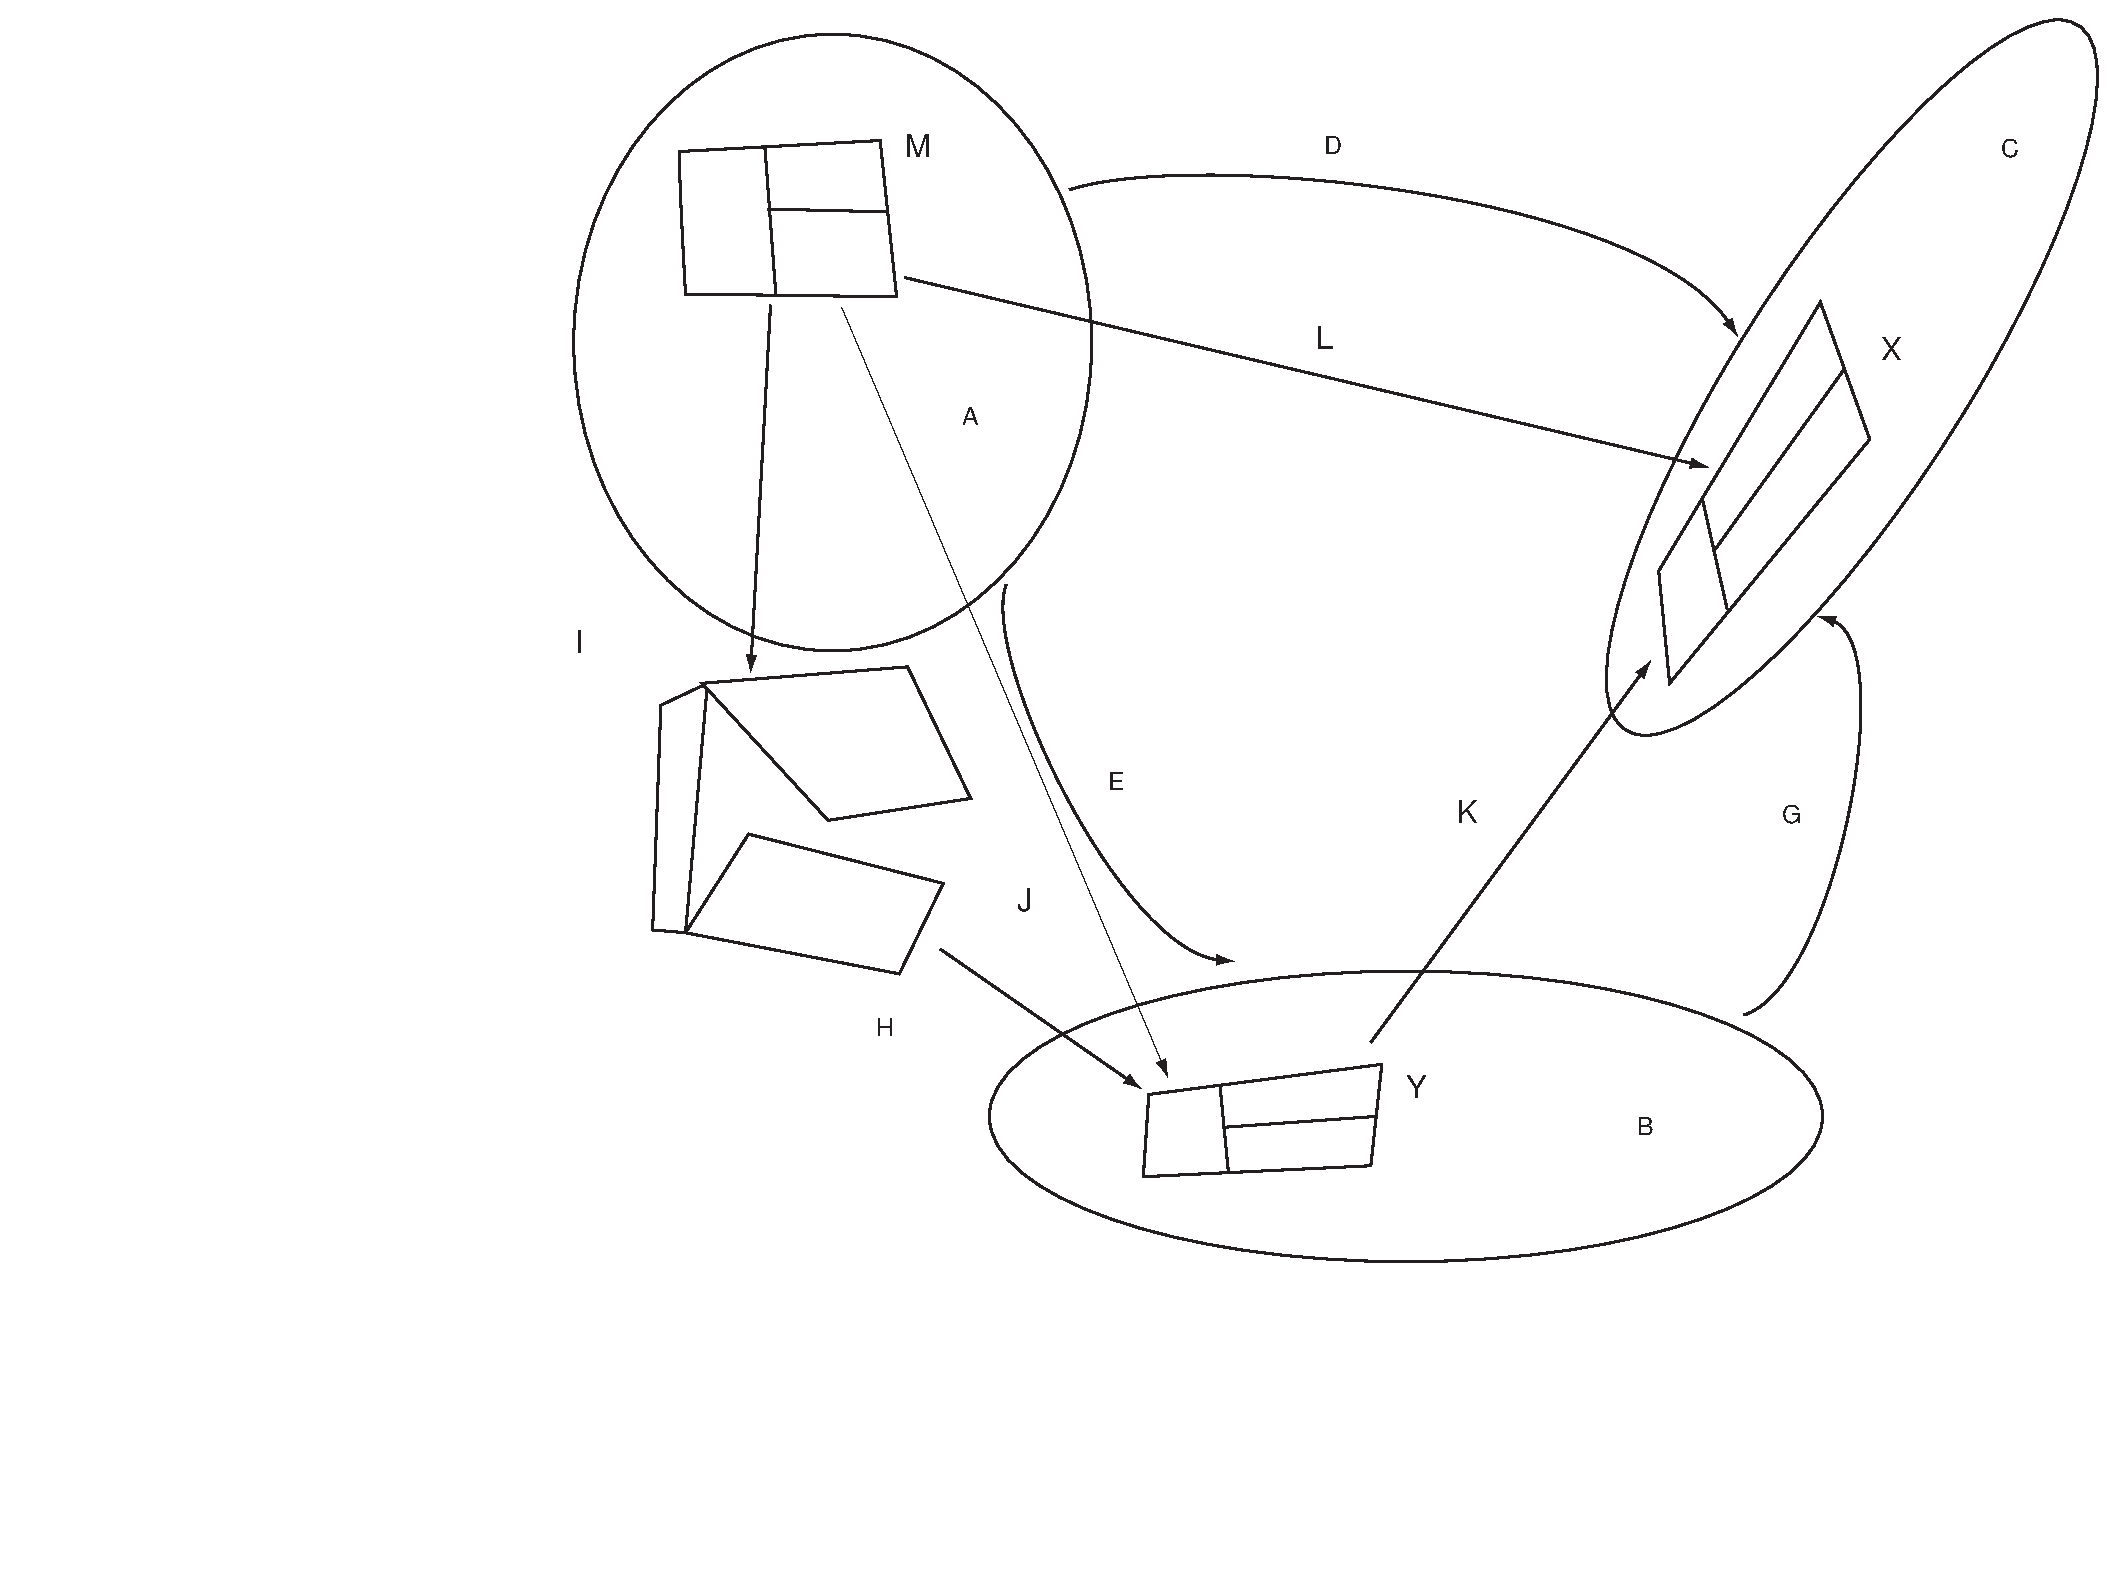
\includegraphics[width=15cm]{images/growthkinematics.eps}} \caption{The
kinematics of growth.} \label{growthkinematicsfig}
\end{figure}

\section{Restrictions on constitutive relations from the
Clausius-Duhem inequality} \label{sect5}

As is the practice in field theories of continuum physics, we use
the Clausius-Duhem inequality (\ref{redentropyineqfin}) to obtain
restrictions on the constitutive relations. We begin with very
general assumptions on the specific internal energy of each
species: $ e^\iota = \hat{e}^\iota(\bF^{\mathrm{e}^\iota},
\eta^\iota, \rho_0^\iota)$. Then, applying the chain rule and
regrouping some terms, (\ref{redentropyineqfin}) becomes
\begin{eqnarray}
& &\sum\limits_{\iota}\left(\frac{\partial
e^\iota}{\partial\bF^{\mathrm{e}^\iota}}-\bP^\iota\bF^{\mathrm{g}^{\iota\mathrm{T}}}\right)\colon\dot{\bF}^{\mathrm{e}^\iota}
+ \sum\limits_{\iota}\left(\frac{\partial e^\iota}{\partial
\eta^\iota}-\theta\right)\frac{\partial\eta^\iota}{\partial t}\nonumber\\
&+&\sum\limits_{\iota} \left(\rho^\iota_0\frac{\partial}{\partial
t}\left(\bV+\bV^\iota\right) - \rho_0^\iota\bg -
\Bnabla\cdot\bP^\iota +
\Bnabla\left(\bV+\bV^\iota\right)\bM^\iota\right)\cdot(\bV^\iota+\bV)\nonumber\\
&+&\sum\limits_{\iota}\left(\rho^\iota_0\bF^{-\mathrm{T}}\left(\Bnabla
e^\iota -
\theta\Bnabla\eta^\iota\right)\right)\cdot\bV^\iota\nonumber\\
&+&\sum\limits_{\iota}\Pi^\iota\left(e^\iota +
\frac{1}{2}\Vert\bV+\bV^\iota\Vert^2\right) +
\frac{\Bnabla\theta\cdot\bQ^\iota}{\theta}\nonumber\\
&+& \sum\limits_{\iota}\rho^\iota_0\frac{\partial
e^\iota}{\partial\rho^\iota_0}\frac{\partial
\rho^\iota_0}{\partial t} -
\sum\limits_{\iota}\bP^\iota\colon(\Bnabla\bV^\iota +
\bF^{\mathrm{e}^\iota}\dot{\bF}^{\mathrm{g}^\iota}) \leq 0.
\label{redentropyineq1}
\end{eqnarray}

\noindent Inequality (\ref{redentropyineq1}) represents a
fundamental restriction upon the physical processes during
biological growth. Any constitutive relations that are prescribed
must satisfy this restriction, as is well-known
\citep{TruesdellNoll:65}. Guided by (\ref{redentropyineq1}), we
prescribe the following constitutive relations in classical form:
\begin{eqnarray}
&&\bP^\iota\bF^{\mathrm{g}^\iota\mathrm{T}} = \rho_0^\iota
\frac{\partial e^\iota}{\partial\bF^{\mathrm{e}^\iota}}
\label{stress-constrelI}\\
\nonumber\\
&&\theta =  \frac{\partial e^\iota}{\partial \eta^\iota},\;\forall\,\iota\label{temp-constrelI}\\
\nonumber\\
&&\rho^\iota_0\bV^\iota =\nonumber\\
& &
-\frac{\tilde{\bD}^\iota}{\rho^\iota_0}\left(\rho^\iota_0\frac{\partial\bV}{\partial
t} - \rho_0^\iota\bg - \Bnabla\cdot\bP^\iota +
\left(\Bnabla\bV\right)\bM^\iota+\rho^\iota_0\bF^{-\mathrm{T}}\left(\Bnabla
e^\iota -
\theta\Bnabla\eta^\iota\right)\right),\label{VIconstrel1}\\
&&\mathrm{where}\;\bw\cdot\tilde{\bD}^\iota\bw
\ge 0,\;\;\forall\, \bw \in\mathbb{R}^3\nonumber\\
\nonumber\\
&&\bQ^\iota = -{\bK}^\iota\Bnabla\theta,\;\bw\cdot{\bK}^\iota\bw
\ge 0,\;\;\forall\, \bw \in\mathbb{R}^3\label{qconstrelI}
\end{eqnarray}

\noindent With the constitutive relations
(\ref{stress-constrelI}--\ref{qconstrelI}) ensuring the
non-positiveness of certain terms the entropy inequality is
further reduced to
\begin{eqnarray}
& & \sum\limits_{\iota}\left(\rho^\iota_0\frac{\partial
e^\iota}{\partial\rho^\iota_0}\frac{\partial
\rho^\iota_0}{\partial t} - \bP^\iota\colon(\Bnabla\bV^\iota +
\bF^{\mathrm{e}^\iota}\dot{\bF}^{\mathrm{g}^\iota})\right)\nonumber\\
&&+\sum\limits_{\iota}\left(
\rho^\iota_0\bV^\iota\cdot\left(\frac{\partial\bV^\iota}{\partial
t} +
\left(\Bnabla\bV^\iota\right)\bF^{-1}\bV^\iota\right)+\Pi^\iota\left(e^\iota
+ \frac{1}{2}\Vert\bV+\bV^\iota\Vert^2\right)\right)\nonumber\\
&&+\sum\limits_{\iota} \left(\rho^\iota_0\frac{\partial}{\partial
t}\left(\bV+\bV^\iota\right) - \rho_0^\iota\bg -
\Bnabla\cdot\bP^\iota +
\Bnabla\left(\bV+\bV^\iota\right)\bM^\iota\right)\cdot\bV \le 0.
\label{dissipation1}
\end{eqnarray}

\noindent The left hand-side of (\ref{dissipation1}) is the
dissipation, $\sD$, a quantity that we will return to below.

Equation (\ref{stress-constrelI}) specifies a constitutive
relation for $\bP^\iota\bF^{\mathrm{g}^{\iota\mathrm{T}}}$, which
is a truly elastic stress. Equation (\ref{temp-constrelI}) implies
a uniform temperature in each species, and corresponds with the
definition usually employed for temperature in thermal physics.
The heat flux in species $\iota$ is given by the product of a
positive semi-definite conductivity tensor, ${\bK}^\iota$ and the
temperature gradient, which is the Fourier Law of heat conduction.
Equation (\ref{VIconstrel1}) requires more detailed discussion
which appears below.

\subsection{Constitutive relations for fluxes}\label{sect5.1}

Turning to (\ref{VIconstrel1}), we first point out that since
$\bM^\iota = \rho_0^\iota\bF^{-1}\bV^\iota$, this is an implicit
relation for $\bV^\iota$. Rewriting it as an explicit one for
$\rho^\iota_0\bV^\iota$ we have,
\begin{eqnarray}
\rho^\iota_0\bV^\iota =& &\left(\bone +
\frac{\tilde{\bD}^\iota\Bnabla\bV\bF^{-1}}{\rho^\iota_0}\right)^{-1}\frac{\tilde{\bD}^\iota}{\rho^\iota_0}\nonumber\\
& &\cdot\left\{-\left(\rho^\iota_0\frac{\partial\bV}{\partial t} -
\rho_0^\iota\bg - \Bnabla\cdot\bP^\iota +
\rho^\iota_0\bF^{-\mathrm{T}}\left(\Bnabla e^\iota -
\theta\Bnabla\eta^\iota\right)\right)\right\}. \label{VIconstrel2}
\end{eqnarray}

\noindent The constitutive relation for flux, $\bM^\iota =
\rho^\iota_0\bF^{-1}\bV^\iota$ is then obtained:
\begin{eqnarray}
\bM^\iota & &=\underbrace{\bF^{-1}\left(\bone +
\frac{\tilde{\bD}^\iota\Bnabla\bV\bF^{-1}}{\rho^\iota_0}\right)^{-1}\frac{\tilde{\bD}^\iota}{\rho^\iota_0}\bF^{-\mathrm{T}}}_{\bD^\iota}\nonumber\\
&\cdot&\left\{\underbrace{-\left(\rho^\iota_0\bF^\mathrm{T}\frac{\partial\bV}{\partial
t} - \rho_0^\iota\bF^\mathrm{T}\bg -
\bF^\mathrm{T}\Bnabla\cdot\bP^\iota + \rho^\iota_0\left(\Bnabla
e^\iota -
\theta\Bnabla\eta^\iota\right)\right)}_{\boldmath{\sF}^\iota}\right\}.
\label{MIconstrel}
\end{eqnarray}

As is common in descriptions of mass transport, the tensor
delineated as $\bD^\iota$ will be referred to as the mobility
tensor of species $\iota$. Recall that in (\ref{VIconstrel1}) we
have taken $\tilde{\bD}^\iota$ to be positive
semi-definite\footnote{If
$\Vert\tilde{\bD}^\iota\Bnabla\bV\bF^{-1}/\rho^\iota_0\Vert << 1$,
we have $\bD^\iota \approx \tilde{\bD}^\iota$.}. The flux is thus
written as the product of a mobility tensor and a thermodynamic
driving force, $\boldmath{\sF}^\iota$. This is the Nernst-Einstein
relation. We proceed now to examine the four separate terms in the
thermodynamic driving force:
\begin{equation}
\boldmath{\sF}^\iota =
-\rho^\iota_0\bF^\mathrm{T}\frac{\partial\bV}{\partial t} +
\rho_0^\iota\bF^\mathrm{T}\bg +
\bF^\mathrm{T}\Bnabla\cdot\bP^\iota - \rho^\iota_0\left(\Bnabla
e^\iota - \theta\Bnabla\eta^\iota\right) \label{drivingforceI}
\end{equation}

\noindent The first two terms respectively represent the
influences of inertia and body force. Thus, the inertial effect is
to drive species $\iota$ in the opposite direction to the body's
acceleration. The body force's influence is directed along itself.
The third term represents the stress divergence effect. In the
case of a non-uniform partial stress, $\bP^\iota$, there exists a
thermodynamic driving force for transport along $\bP^\iota$. We
demonstrate this effect for the case of the fluid species in
Section \ref{sect5.2} below, for which it translates to the more
intuitive notion of transport along a fluid pressure gradient.

The fourth term in $\boldmath{\sF}^\iota$ admits the following
interpretation: The Legendre transformation $\psi^\iota = e^\iota
- \theta\eta^\iota$ allows one to rewrite $\Bnabla e^\iota -
\theta\Bnabla\eta^\iota$ as $\Bnabla\psi^\iota\vert_\theta$ (at
uniform temperature), where $\psi^\iota$ is the mass-specific
Helmholtz free energy. An assumption inherent in the development
that began in Section \ref{sect2} is that any mass entering or
leaving $\Omega_0$ at a point $\bX$ on the boundary,
$\partial\Omega_0$, has the field values
$\rho_0^\iota,e^\iota,\eta^\iota,\theta$, and $\psi^\iota$
corresponding to $\bX$. Likewise, the incremental mass of species
$\iota$ created or absorbed via the source/sink $\Pi^\iota$ at
$\bX$ has the field values of that point. Consider a sufficiently
small neighborhood of a point, say
$\mathsf{N}(\bX)\subset\Omega_0$. Changing the mass of species
$\iota$ in $\mathsf{N}(\bX)$ by $\delta\mathsf{m}^\iota$ units
causes a change in the Helmholtz free energy of $\iota$ in
$\mathsf{N}(\bX)$ by $\delta\Psi^\iota =
\psi^\iota\delta\mathsf{m}^\iota$. By definition therefore,
$\psi^\iota =
\partial\Psi^\iota/\partial\mathsf{m}^\iota$. This derivative gives the \emph{chemical
potential}, $\mu^\iota$, of the transported species, $\iota$.
Thus, we have $\mu^\iota = e^\iota - \theta\eta^\iota$, and
$\Bnabla e^\iota -\theta\Bnabla\eta^\iota =
\Bnabla\mu^\iota\vert_\theta$. This last term in
${\boldmath{\sF}}^\iota$ thus represents the thermodynamic driving
force due to a chemical potential gradient.

It has recently come to our attention that the constitutive
relation for flux (\ref{MIconstrel}) is precisely the result
arrived at by \citet{DeGrootMazur:1984}, including the
identification of the chemical potential gradient term. However,
their approach involves a slightly different application of the
Second Law, and a less detailed treatment of the mechanics.

The gradient of internal energy in (\ref{drivingforceI}) leads to
a strain gradient-dependent term. A concentration gradient-driven
term arises from the gradient of mixing entropy. Together with the
other terms that were remarked upon above, they represent a
complete thermodynamic formulation of coupled mass transport and
mechanics. This is the central result of our paper.

\subsection{Transport of the fluid species: The example of an ideal fluid}\label{sect5.2}

Consider the stress divergence term
$\bF^\mathrm{T}\Bnabla\cdot\bP^\iota$. An elementary calculation
gives
\begin{equation}
\bF^\mathrm{T}\Bnabla\cdot\bP^\iota =
\Bnabla\cdot\left(\bF^\mathrm{T}\bP^\iota\right) -
\Bnabla\bF^\mathrm{T}\colon\bP^\iota. \label{stressdivI}
\end{equation}

\noindent In indicial form, where lower/upper case indices are for
components of quantities in the current/reference configuration
respectively, this relation is
\begin{displaymath}
F_{iK}P^\iota_{iJ,J} = \left(F_{iK}P^\iota_{iJ}\right)_{,J} -
F_{iK,J}P^\iota_{iJ}.
\end{displaymath}

\noindent For an ideal fluid, supporting only an isotropic Cauchy
stress, $p\bone$, we have $\bP^\mathrm{f} =
\mathrm{det}(\bF)p\bF^{-\mathrm{T}}$, where $p$ is positive in
tension. The arguments that follow assume this case. (The more
general case of a non-ideal, viscous fluid will merely have
additional terms from the viscous Cauchy stress.) The stress
divergence term is
\begin{equation}
\bF^\mathrm{T}\Bnabla\cdot\bP^\mathrm{f} =
\Bnabla\left(\mathrm{det}(\bF)p\right) -
\Bnabla\bF^\mathrm{T}\colon\bF^{-\mathrm{T}}\mathrm{det}(\bF)p,
\end{equation}

\noindent demonstrating the appearance of a hydrostatic
stress-driven contribution to ${\boldmath{\sF}}^\mathrm{f}$. This
is Darcy's Law for transport of a fluid down a pressure gradient.

For the special case of a compressible, ideal fluid we have
$e^\mathrm{f} =
\bar{e}^\mathrm{f}(\eta^\mathrm{f},\bar{\rho}^\mathrm{f})$; i.e.,
the fluid stores strain energy as a function of its \emph{current,
intrinsic} density. Fluid saturation conditions hold in biological
tissue, for which case the fluid volume fraction, $f^\mathrm{f}$,
is simply the pore volume fraction. Recall from Section
\ref{sect2} that the individual species deform with the common
deformation gradient $\bF$. Therefore the pores deform
\emph{homogeneously} with the surrounding solid phase. Physically
this corresponds to the pore size being smaller than the scale at
which the homogenization assumption of a continuum theory holds.
Momentarily ignoring changes in reference concentration of the
fluid, we have $\bF^{\mathrm{e}^\mathrm{f}} = \bF$.  Then, since
$\rho^\mathrm{f}_0 = \bar{\rho}^\mathrm{f}_0 f^\mathrm{f}$, we can
write $\hat{e}^\mathrm{f}(\bF,\eta^\mathrm{f},\rho^\mathrm{f}_0) =
\hat{e}^\mathrm{f}(\bF,\eta^\mathrm{f},\bar{\rho}^\mathrm{f}_0
f^\mathrm{f}) =
\bar{e}^\mathrm{f}(\eta^\mathrm{f},\bar{\rho}^\mathrm{f}_0/\mathrm{det}\bF)=
\bar{e}^\mathrm{f}(\eta^\mathrm{f},\bar{\rho}^\mathrm{f})$. In
this case a simple calculation shows that the hydrostatic pressure
is
\begin{displaymath}
p =
-\frac{\bar{\rho}^\mathrm{f}}{\mathrm{det}(\bF)}\frac{\partial\bar{e}^\mathrm{f}}{\partial\bar{\rho}^\mathrm{f}},
\end{displaymath}

\noindent and the stress divergence term is
\begin{displaymath}
\bF^\mathrm{T}\Bnabla\cdot\bP^\mathrm{f} =
-\Bnabla\left(\bar{\rho}^\mathrm{f}\frac{\partial\bar{e}^\mathrm{f}}{\partial\bar{\rho}^\mathrm{f}}\right)
+
\Bnabla\bF^\mathrm{T}\colon\bF^{-\mathrm{T}}\bar{\rho}^\mathrm{f}\frac{\partial\bar{e}^\mathrm{f}}{\partial\bar{\rho}^\mathrm{f}}.
\end{displaymath}

\subsection{The Eshelby stress as a thermodynamic driving
force}\label{sect5.3}

Combining the stress divergence and chemical potential gradient
contributions to the driving force for any species, and using the
mass-specific Helmholtz free energy, $\psi^\iota$, we write,

\begin{equation}
\bF^\mathrm{T}\Bnabla\cdot\bP^\iota - \rho^\iota_0\left(\Bnabla
e^\iota - \theta\Bnabla\eta^\iota\right) =
\Bnabla\cdot\left(\bF^\mathrm{T}\bP^\iota\right) -
\Bnabla\bF^\mathrm{T}\colon\bP^\iota
 - \rho^\iota_0\Bnabla\psi^\iota\vert_\theta.
\end{equation}

\noindent Regrouping terms this expression is
\begin{equation}
-\Bnabla\cdot\underbrace{\left(\rho^\iota_0\psi^\iota\vert_\theta\bone
- \bF^\mathrm{T}\bP^\iota\right)}_{\mbox{Eshelby
stress},\;\BXi^\iota} +
\left(\Bnabla\rho^\iota_0\right)\psi^\iota_0\vert_\theta -
\Bnabla\bF^\mathrm{T}\colon\bP^\iota.
\end{equation}

Thus, the divergence of the well-known Eshelby stress tensor is
also among the driving forces for mass transport. Also observe the
presence of a strain gradient-dependent driving force,
$-\Bnabla\bF^\mathrm{T}\colon\bP^\iota$ in the developments of
Sections \ref{sect5.2} and \ref{sect5.3}, independent of the
pressure gradient term for the fluid species.


\noindent{\bf Remark 1}: The final version of the dissipation
inequality (\ref{dissipation1}), and the mass balance equation can
be manipulated to restrict the mathematical form of the mass
source. It is common to make the mass source depend upon the
strain energy density \citep{HarriganHamilton:1993} while
respecting the restriction imposed by the dissipation inequality.
This form is often used while modelling hard tissue. Such an
approach leads to strain-mediated mass transport. However, with a
strain-independent source, strain-mediated (or stress-mediated)
mass transport would not be obtained with such a formulation.

\noindent{\bf Remark 2}: We expect that evaluation of the
dissipation, $\sD$, using (\ref{dissipation1}) from field
quantities in a boundary value problem will provide a test of
soundness, and if necessary indications for improvement, of our
constitutive models.

\noindent{\bf Remark 3}: Since soft biological tissues usually
demonstrate rate-dependent response, it has been common to employ
a solid viscoelastic constitutive model for them. This approach
fits within our framework, with a modification of the internal
energy to include its dependence upon internal variables that
represent the viscoelastic stress-like parameters. However, a more
physiologically-valid model may be one with a purely hyperelastic
solid phase, and a viscous fluid. In such a composite model the
rate-dependent behavior would arise from the fluid.

\noindent{\bf Remark 4}: The constitutive relations
(\ref{stress-constrelI}) and (\ref{MIconstrel}) respectively
specify the partial stress, $\bP^\iota$, and flux, $\bM^\iota$, of
a species. The flux also implies the relative velocity,
$\bV^\iota$. The velocity of the solid phase, $\bV$ is obtained
from the local form of the balance of linear momentum for the
system (\ref{linmombalsys}). With all these quantities known, the
individual interaction forces between species,
$\rho^\iota_0\bq^\iota$, can be obtained from
(\ref{ballinmomrefI}). They are, however, not needed while solving
for the balance of linear momentum of the system.

\section{A numerical example} \label{sect6}

The theory developed in Sections \ref{sect2}--\ref{sect5} has been
implemented in a computational formulation, retaining much of the
complexity of the coupled balance laws and constitutive relations.
For realistic soft tissue material parameters, the contribution of
the fluxes and interaction forces between species to the balance
of linear momentum of the composite tissue is negligible. This
simplification has been used. As a preliminary demonstration of
the theory\footnote{This numerical section has been included
mainly for completeness of this theoretical paper. A separate
paper, currently in preparation, will present the computational
formulation and contain a detailed examination of a number of
initial and boundary value problems for growth.}, we present a
computation of the coupled physics in the early stages of uniaxial
extension of a cylindrical soft tissue specimen. The motivation
for this model problem comes from our experimental model of
engineered, functional tendon constructs grown \emph{in vitro},
having the same cylindrical geometry. The experimental aspects of
our broad-based project on soft tissue growth are described
elsewhere \citep{Calve:04}. In addition to engineering
scaffold-less tendon constructs from neonatal rat fibroblast
cells, we have the ability to impose a range of mechanical,
chemical, nutritional and electrical stimuli on them and study the
tissue's response. Besides modelling these experiments, the
mathematical formulation described here presents researchers with
a vehicle for testing scenarios and framing hypotheses that can be
experimentally-validated in our laboratory, thereby driving the
experimental studies.

\subsection{Material models and parameters}\label{sect6.1}

The engineered tendon construct is $12$ mm in length and
$1\;\mathrm{mm}^2$ in area. In this paper an internal energy
density for the solid phase based upon the worm-like chain model
is used. The reader is directed to \citet{Riefetal:97} and
\cite{Bustamanteetal:2003} where the one-dimensional version of
this model has been applied to long chain molecules. It has been
described and implemented into an anisotropic representative
volume element by \citet{Bischoffetal:2002}, and is summarized
here. The internal energy density of a single constituent chain of
an eight-chain model (Figure \ref{eightchain}) is,
\begin{eqnarray}
\bar{\rho}_0^\mathrm{s}\hat{e}^\mathrm{s}(\bF^{\mathrm{e}^\mathrm{s}},\rho_0^\mathrm{s},\eta^\mathrm{s})
&=& \frac{N k \theta}{4 A}\left(\frac{r^2}{2L} +
\frac{L}{4(1-r/L)} -
\frac{r}{4}\right)\nonumber\\
&-&\frac{N k \theta}{4\sqrt{2L/A}}\left(\sqrt{\frac{2A}{L}} +
\frac{1}{4(1 - \sqrt{2A/L})} -\frac{1}{4} \right)\log(\lambda_1^{a^2}\lambda_2^{b^2}\lambda_3^{c^2})\nonumber\\
&+& \frac{\gamma}{\beta}({J^{\mathrm{e}^\mathrm{s}}}^{-2\beta} -1)
+ 2\gamma{\bf 1}\colon\bE^{\mathrm{e}^\mathrm{s}} \label{wlcmeq}
\end{eqnarray}
\noindent Here, $N$ is the density of chains, $k$ is the Boltzmann
constant, $r$ is the end-to-end length of a chain, $L$ is the
fully-extended length, and $A$ is the persistence length that
measures the degree to which the chain departs from a straight
line. The preferred orientation of tendon collagen is described by
an anisotropic unit cell with sides $a,b$ and $c$---see Figure
\ref{eightchain}. All lengths in this model have been rendered
non-dimensional (Table \ref{mattab}) by dividing by the link
length in a chain.
\begin{figure}[ht]
\psfrag{A}{$a$} \psfrag{B}{$b$} \psfrag{C}{$c$} \centering
{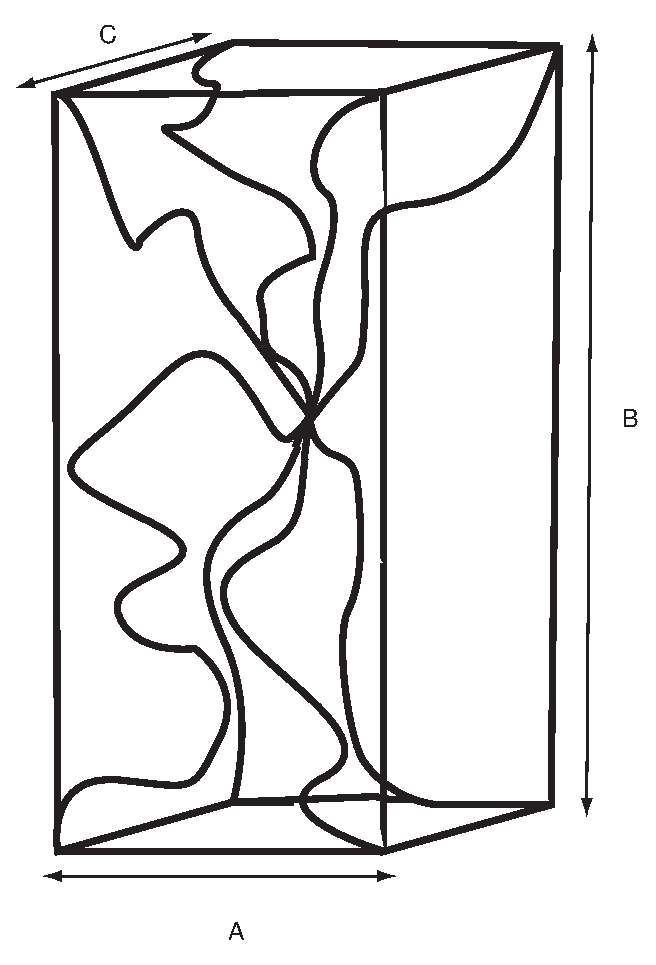
\includegraphics[width=3.5cm]{images/wlcm.eps}} \caption{Worm-like
chains grouped into an initially anisotropic eight-chain model.}
\label{eightchain}.
\end{figure}

The elastic stretches along the unit cell axes are respectively
denoted $\lambda^\mathrm{e}_1,\lambda^\mathrm{e}_2$ and
$\lambda^\mathrm{e}_3$, and $\bE^{\mathrm{e}^\mathrm{s}} =
\frac{1}{2}(\bC^{\mathrm{e}^\mathrm{s}} - {\bf 1})$ is the elastic
Lagrange strain. The factors $\gamma$ and $\beta$ control bulk
compressibility. The end-to-end length is given by

\begin{equation}
r =
\frac{1}{2}\sqrt{a^2\lambda_1^{\mathrm{e}^2}+b^2\lambda_2^{\mathrm{e}^2}+c^2\lambda_3^{\mathrm{e}^2}},\quad
\lambda_I^{\mathrm{e}} = \sqrt{\bN_I\cdot\bC^{\mathrm{e}}\bN_I}
\label{rwlcm}
\end{equation}

Preliminary mechanical tests of the engineered tendon have been
carried out in our laboratory but, at this stage, the worm-like
chain model has not been calibrated to these tests. Instead,
published data for the worm-like chain, obtained by calibrating
against rat cardiac tissue  \citep{Bischoffetal:2002}, has been
employed.

The fluid phase was modelled as an ideal, nearly-incompressible
fluid:
\begin{equation}
\bar{\rho}^\mathrm{f}_0\hat{e}^\mathrm{f}(\bF^{\mathrm{e}^\mathrm{f}},\rho_0^\mathrm{f},\eta^\mathrm{f})
=
\frac{1}{2}\kappa(\mathrm{det}(\bF^{\mathrm{e}^\mathrm{f}})-1)^2,
\end{equation}

\noindent where $\kappa$ is the fluid bulk modulus.

Only a solid and a fluid phase were included for the tissue. Low
values were chosen for the mobilities of the fluid
\citep{Swartzetal:99} with respect to the solid phase (see Table
\ref{mattab}). In order to demonstrate growth, the solid phase
must have a source term, $\Pi^\mathrm{s}$ (Section \ref{sect2}),
and the only other phase, the fluid, must have $\Pi^\mathrm{f} =
-\Pi^\mathrm{s}$. Therefore, contrary to the case made in Section
\ref{sect2}, a non-zero value of the fluid source,
$\Pi^\mathrm{f}$, was assumed. A form motivated by first-order
reactions was used:
\begin{equation}
\Pi^\mathrm{f} = -k^\mathrm{f}(\rho_0^\mathrm{f} -
\rho_{0_\mathrm{ini}}^\mathrm{f}),\quad \Pi^\mathrm{s} =
-\Pi^\mathrm{f}, \label{piform}
\end{equation}

\noindent where $k^\mathrm{f}$ is the reaction rate, and
$\rho_{0_\mathrm{ini}}^\mathrm{f}$ is the initial fluid
concentration. This term acts as a source for the solid when
$\rho_0^\mathrm{f}
> \rho_{0_\mathrm{ini}}^\mathrm{f}$, and a sink when
$\rho_0^\mathrm{f} < \rho_{0_\mathrm{ini}}^\mathrm{f}$.

In a very simple approximation, the fluid's mixing entropy was
written as
\begin{equation}
\eta^\mathrm{f}_\mathrm{mix} =
-\frac{k}{\sM^\mathrm{f}}\log\frac{\rho_0^\mathrm{f}}{\rho_0}.
\label{mixentropy}
\end{equation}

\noindent Recall that in the notation of Section \ref{sect2},
$\sM^\mathrm{f}$ is the fluid's molecular weight.

\begin{table}[ht]
\caption{Material parameters used in the analysis} \label{mattab}
\begin{tabular}{lcll}
\hline
\multicolumn{1}{c}{Parameter} & Symbol & Value & Units\\
\hline
Chain density & $N$ & $7\times 10^{21}$ & $\mathrm{m}^{-3}$\\
Temperature& $\theta$  & $310.0$ & K\\
Persistence length & $A$ & $1.3775$ & --\\
Fully-stretched length & $L$ & $25.277$ & --\\
Unit cell axes & $a,\;b,\;,c$ & $9.2981,\;12.398,\;6.1968$ & --\\
Bulk compressibility factors & $\gamma,\;\beta$ & $1000,\; 4.5$ & --\\
Fluid bulk modulus &$\kappa$ & $1$ & GPa\\
Fluid mobility tensor components& $D_{11},\;D_{22},\;D_{33}$ & $1\times 10^{-8},\;1\times 10^{-8},\;1\times 10^{-8}$ &$\mathrm{m}^{-2}\mathrm{sec}$\\
Fluid conversion reaction rate & $k^\mathrm{f}$ & $-1.\times 10^{-7}$ & $\mathrm{sec}^{-1}$\\
Gravitational acceleration & $\bg$ & $9.81$ & $\mathrm{m}.\mathrm{sec}^{-2}$\\
Molecular weight of fluid &$\sM^\mathrm{f}$& $2.9885\times 10^{-23}$ & $\mathrm{kg}$\\
\hline
\end{tabular}
\end{table}

\subsection{Boundary and initial conditions; coupled solution method}\label{sect6.2}

Boundary conditions for mass transport consisted of the specified
fluid concentration at all external surfaces of the cylinder. This
value was fixed at $500\,\mathrm{kg.m}^{-3}$. With these boundary
conditions the fluid flux normal to surfaces of the specimen is
determined by solving the initial and boundary value problem. The
bottom planar surface was fixed in the $\be_3$ direction and a
displacement was applied at the top surface, also in the $\be_3$
direction, to give a nominal strain rate of
$0.05\,\mathrm{sec}^{-1}$ in the $\be_3$ direction. This is the
only mechanical load on the problem. Initial conditions were
$\rho_0^\mathrm{f}(\bX,0) =
500\,\mathrm{kg.m}^{-3},\;\rho_0^\mathrm{s}(\bX,0) =
500\,\mathrm{kg.m}^{-3}$, and for the mechanical problem,
$\bu(\bX,0) = \bzero,\,\bV(\bX,0) = \bzero$.

The coupled problem was solved by a staggered scheme based upon
operator splits \citep{Armero:99,Garikipatietal:01}. The details
will be presented in a future communication that will focus upon
computational aspects and numerical examples. Here we only mention
that the staggered scheme consists of identifying the displacement
and species concentrations as primitive variables associated with
the mechanical and mass transport problems. The mechanical problem
is solved holding the concentrations fixed. The resulting
displacement field is then held constant to solve the mass
transport problem. The transient solution is obtained for
mechanics using energy-momentum conserving schemes
\citep{SimoTarnow:1992b,SimoTarnow:1992a,Gonzalezphd:1996}, and
for mass transport using the Backward Euler Method. Hexahedral
elements are employed, combined with nonlinear projection methods
\citep{simotaylorpister:85} to treat the near-incompressibility
imposed by the fluid. The numerical formulation has been
implemented within the nonlinear finite element program, FEAP
\citep{feapmanual}.

\subsection{Evolution of stress and flux}\label{sect6.3}

The following contour plots represent the stress, and various
contributions to the total flux in the early stages of loading of
the model problem. Symmetry has been employed to model a single
quadrant of the cylinder.

The longitudinal stress, $\sigma_{33}$ in Figure \ref{stressfig}
arises from the stretch and the evolution in concentration.
\begin{figure}[ht]
\begin{minipage}[t]{7.5cm}
{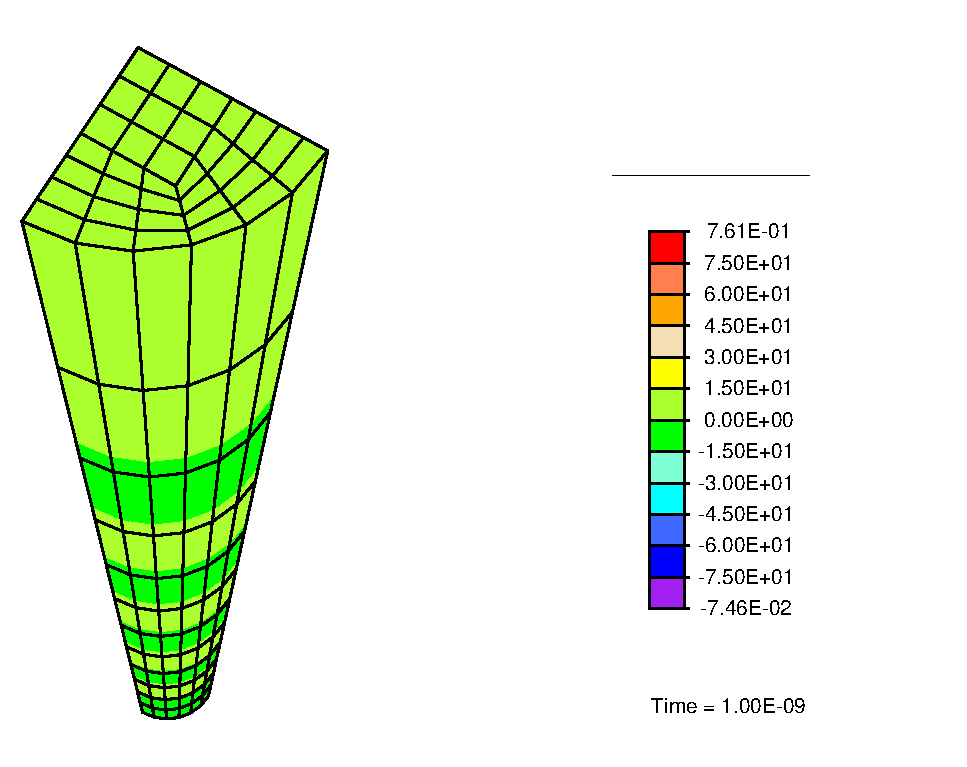
\includegraphics[width=7.5cm]{images/S33-1.eps}} \hskip 3cm (a)
\end{minipage}
\begin{minipage}[t]{7.5cm}
{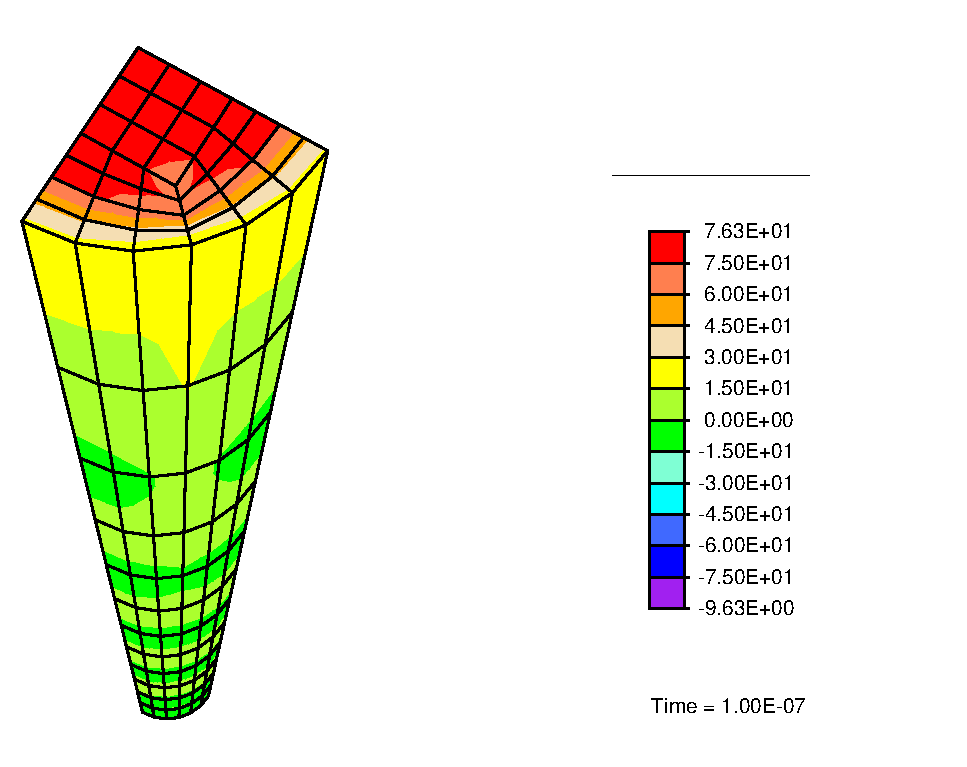
\includegraphics[width=7.5cm]{images/S33-100.eps}} \hskip 3cm (b)
\end{minipage}
\caption{Longitudinal Cauchy stress, $\sigma_{33}$ (Pa) at $1
\,\mathrm{nanosec.}$ and $100\,\mathrm{nanosec.}$ after the
beginning of loading.} \label{stressfig}
\end{figure}

\begin{figure}[ht]
\begin{minipage}[t]{7.5cm}
{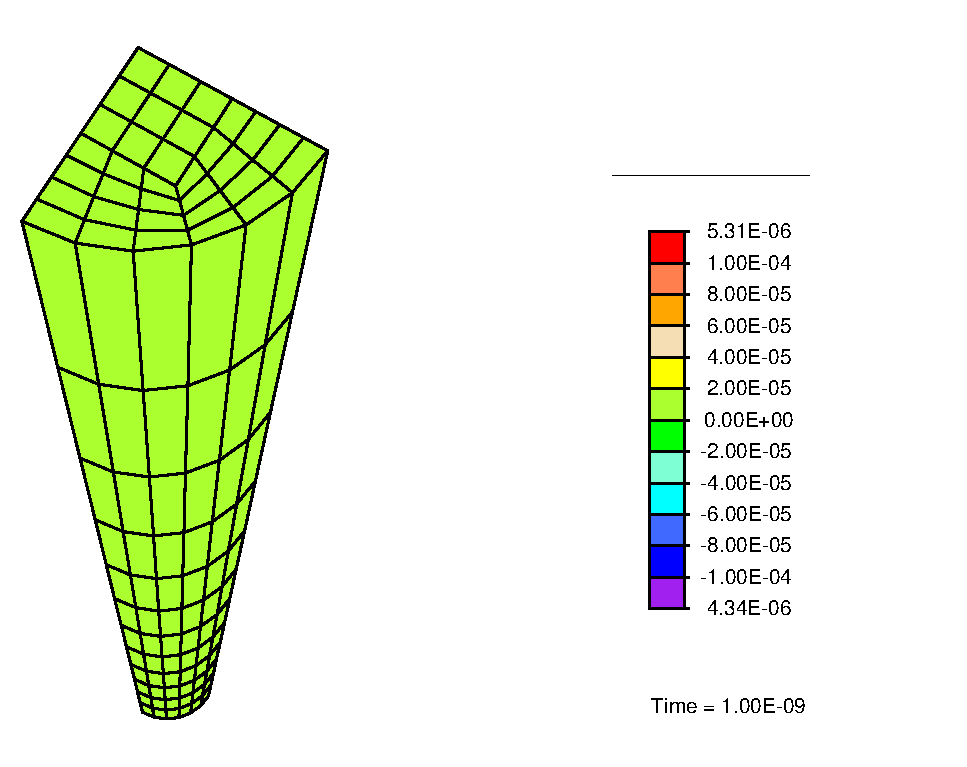
\includegraphics[width=7.5cm]{images/M1-1.eps}} \hskip 3cm (a)
\end{minipage}
\begin{minipage}[t]{7.5cm}
{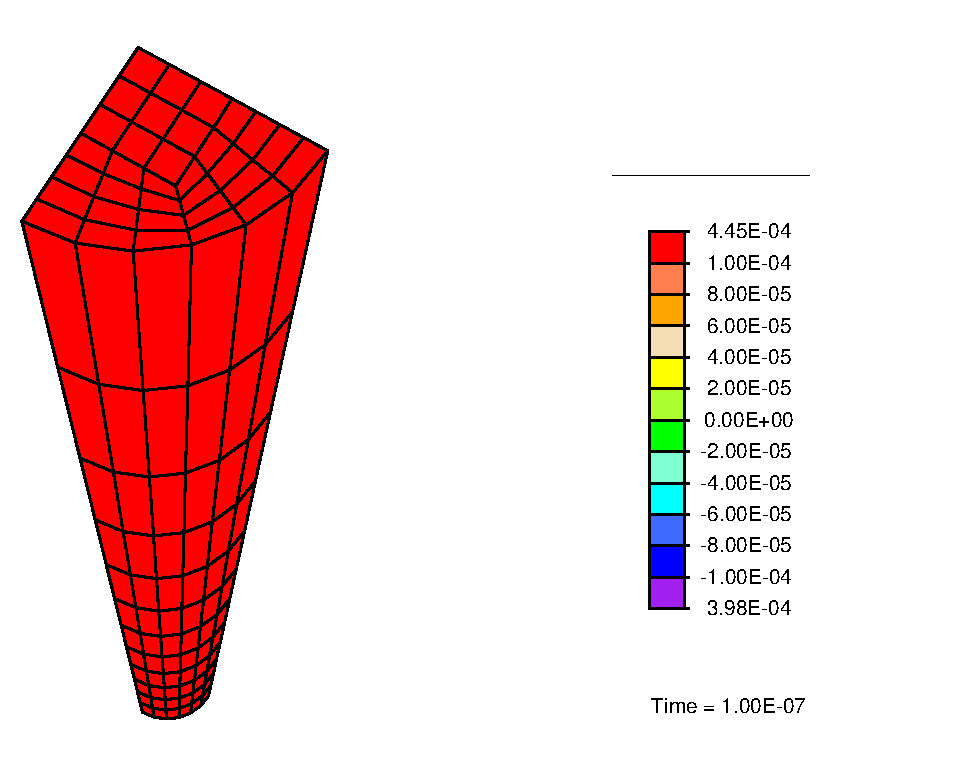
\includegraphics[width=7.5cm]{images/M1-100.eps}} \hskip 3cm (b)
\end{minipage}
\caption{Stress gradient-driven flux
($\mathrm{kg.m}^{-2}\mathrm{sec}$) in the $\be_3$ direction at $1
\,\mathrm{nanosec.}$ and $100\,\mathrm{nanosec.}$ after the
beginning of loading. The positive values indicate an upward flux
corresponding to a tensile $\sigma_{33}$ wave travelling
downwards.} \label{M1fig}
\end{figure}

\begin{figure}[ht]
\begin{minipage}[t]{7.5cm}
{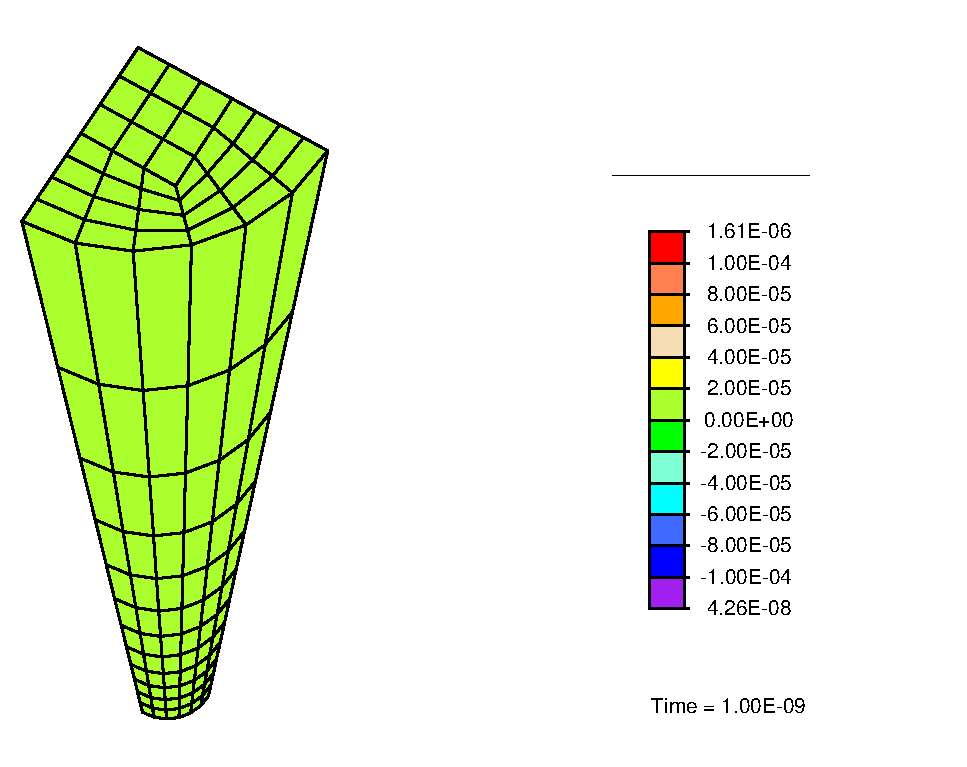
\includegraphics[width=7.5cm]{images/M2-1.eps}} \hskip 3cm (a)
\end{minipage}
\begin{minipage}[t]{7.5cm}
{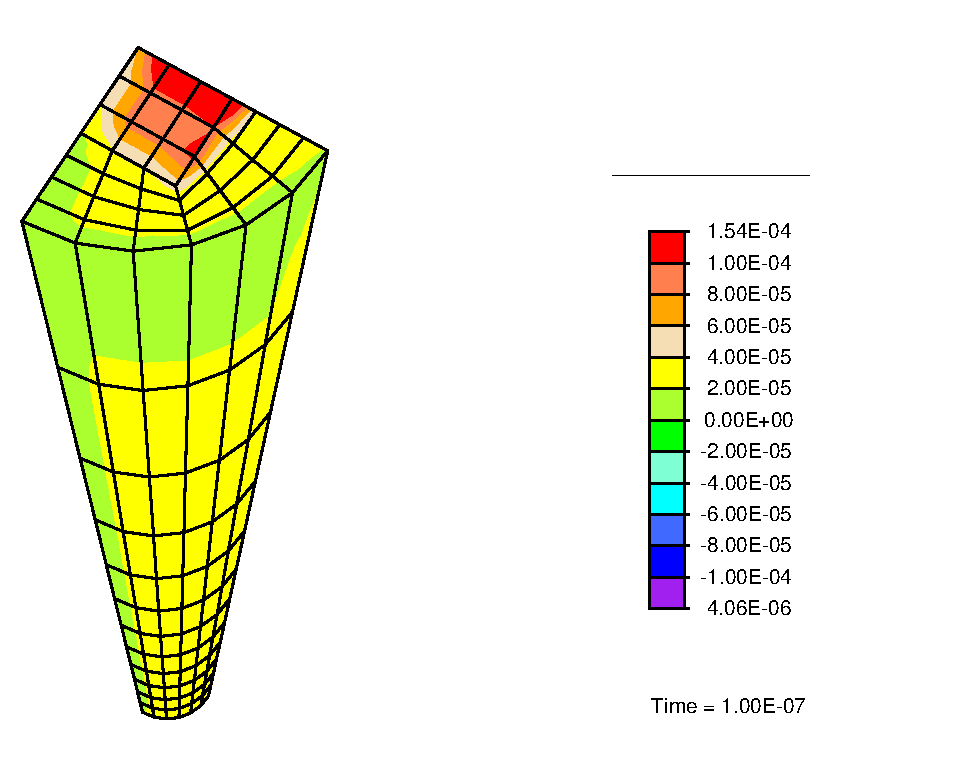
\includegraphics[width=7.5cm]{images/M2-100.eps}} \hskip 3cm (b)
\end{minipage}
\caption{Internal energy gradient-driven flux,
($\mathrm{kg.m}^{-2}\mathrm{sec}$) in the $\be_3$ direction at $1
\,\mathrm{nanosec.}$ and $100\,\mathrm{nanosec.}$ after the
beginning of loading. The positive values indicate an upward flux.
This corresponds to a lower energy near the top of the cylinder as
the tensile stress ($\sigma_{33}$) wave travels downward and
relaxes some of the strain energy of contraction.} \label{M2fig}
\end{figure}

\begin{figure}[ht]
\begin{minipage}[t]{7.5cm}
{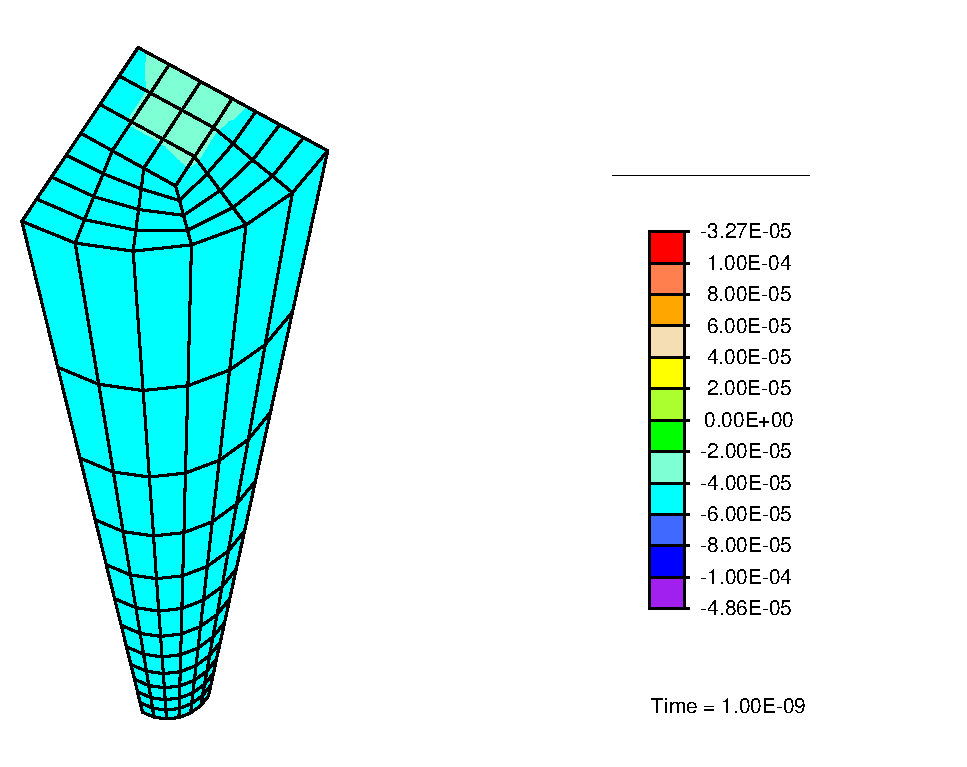
\includegraphics[width=7.5cm]{images/M3-1.eps}} \hskip 3cm (a)
\end{minipage}
\begin{minipage}[t]{7.5cm}
{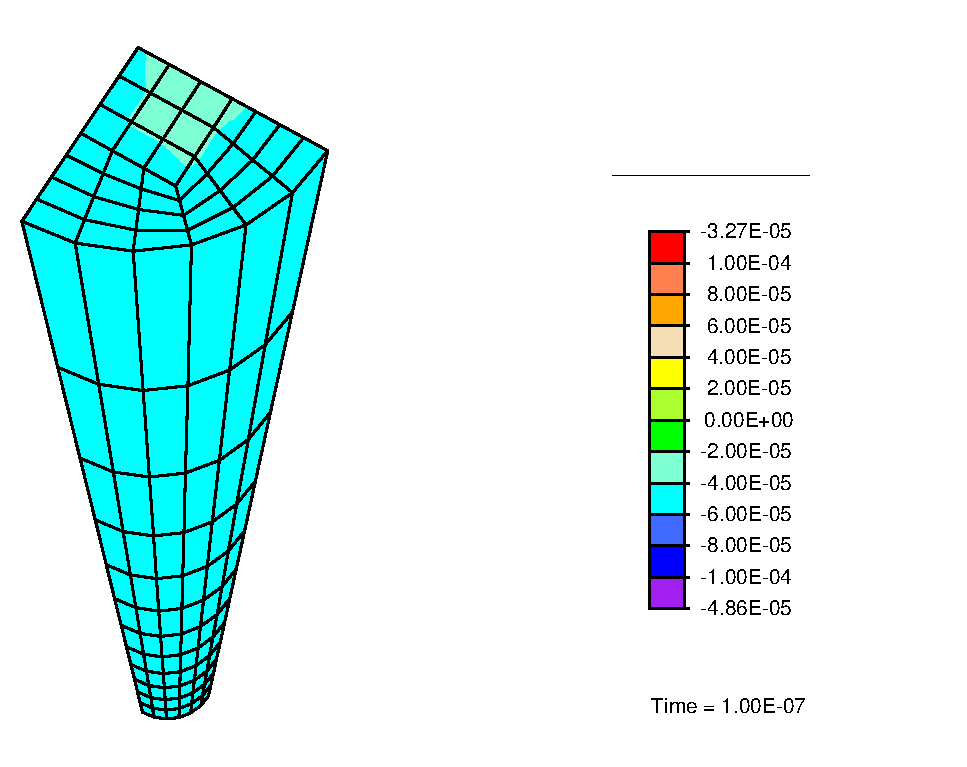
\includegraphics[width=7.5cm]{images/M3-100.eps}} \hskip 3cm (b)
\end{minipage}
\caption{Gravity-driven flux ($\mathrm{kg.m}^{-2}\mathrm{sec}$) in
the $\be_3$ direction at $1 \,\mathrm{nanosec.}$ and
$100\,\mathrm{nanosec.}$ after the beginning of loading. The
negative values indicate a downward flux, due to the action of
gravity.} \label{M3fig}
\end{figure}

\begin{figure}[ht]
\begin{minipage}[t]{7.5cm}
{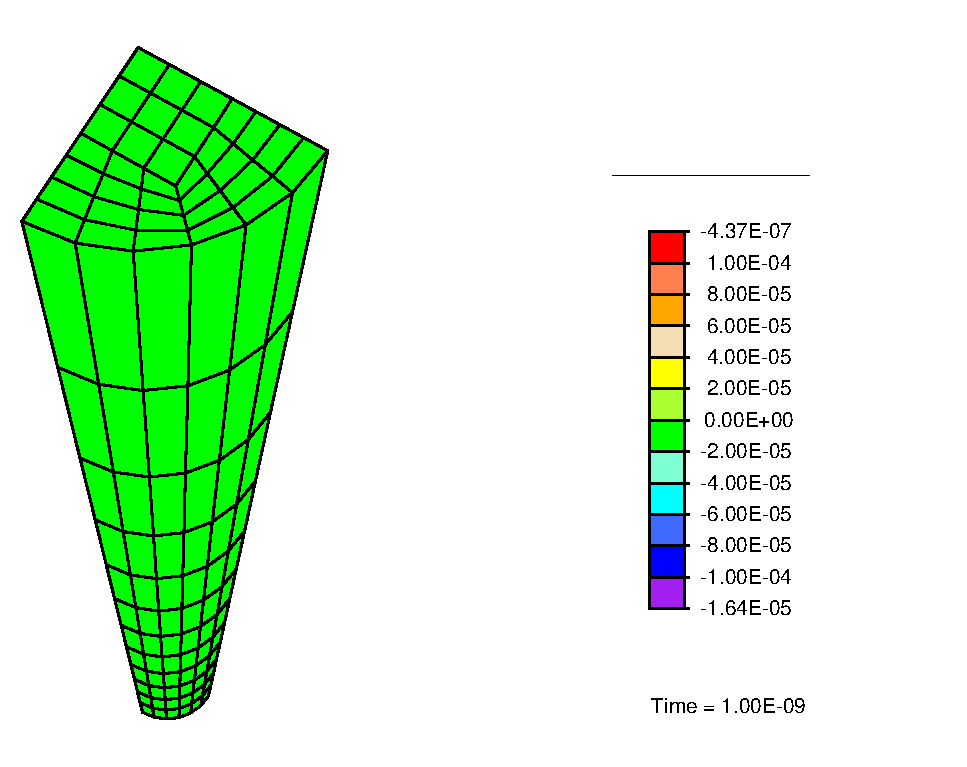
\includegraphics[width=7.5cm]{images/M4-1.eps}} \hskip 3cm (a)
\end{minipage}
\begin{minipage}[t]{7.5cm}
{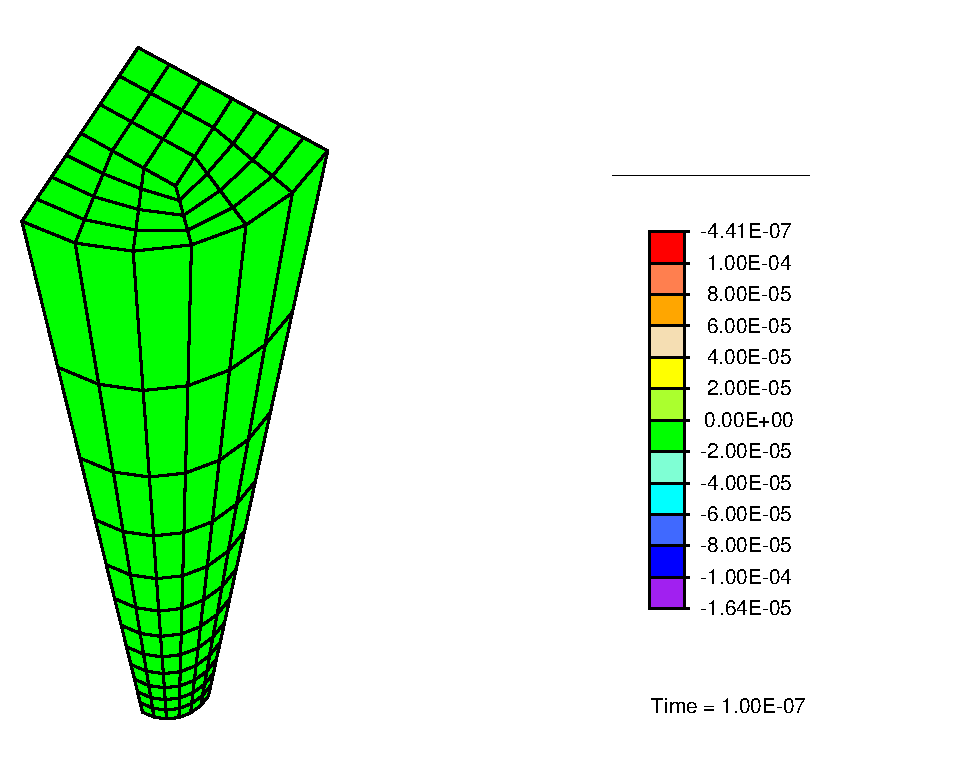
\includegraphics[width=7.5cm]{images/M4-100.eps}} \hskip 3cm (b)
\end{minipage}
\caption{Inertia-driven flux ($\mathrm{kg.m}^{-2}\mathrm{sec}$) in
the $\be_3$ direction at $1 \,\mathrm{nanosec.}$ and
$100\,\mathrm{nanosec.}$ after the beginning of loading. The
negative values indicate a downward flux as the tissue accelerates
upward.} \label{M4fig}
\end{figure}

\begin{figure}[ht]
\begin{minipage}[t]{7.5cm}
{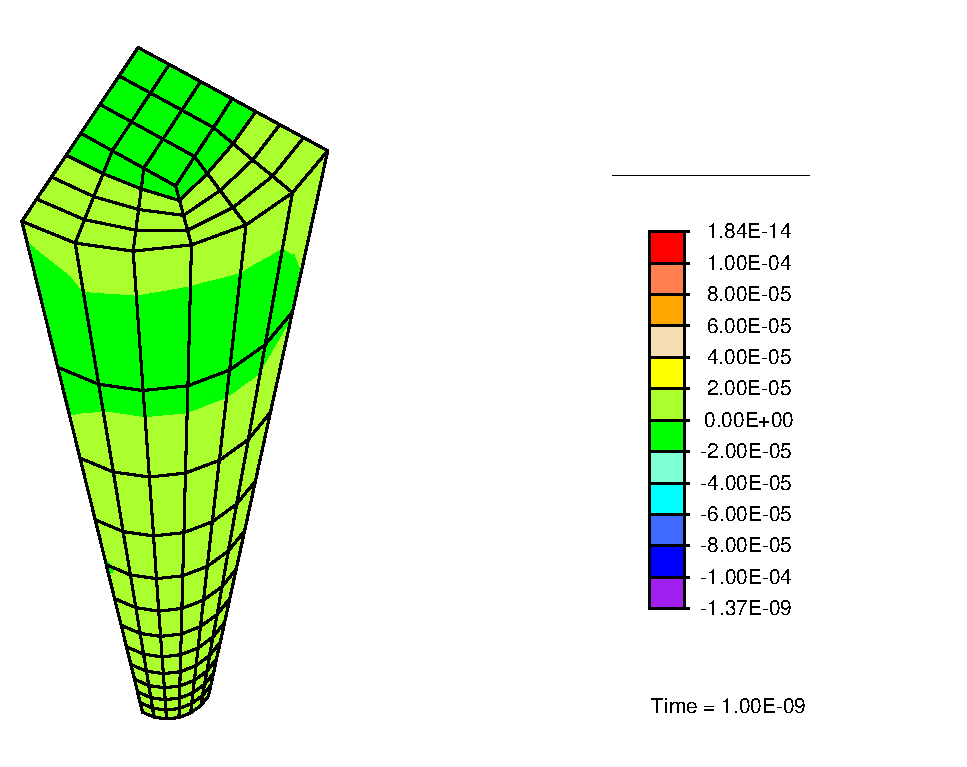
\includegraphics[width=7.5cm]{images/M5-1.eps}} \hskip 3cm (a)
\end{minipage}
\begin{minipage}[t]{7.5cm}
{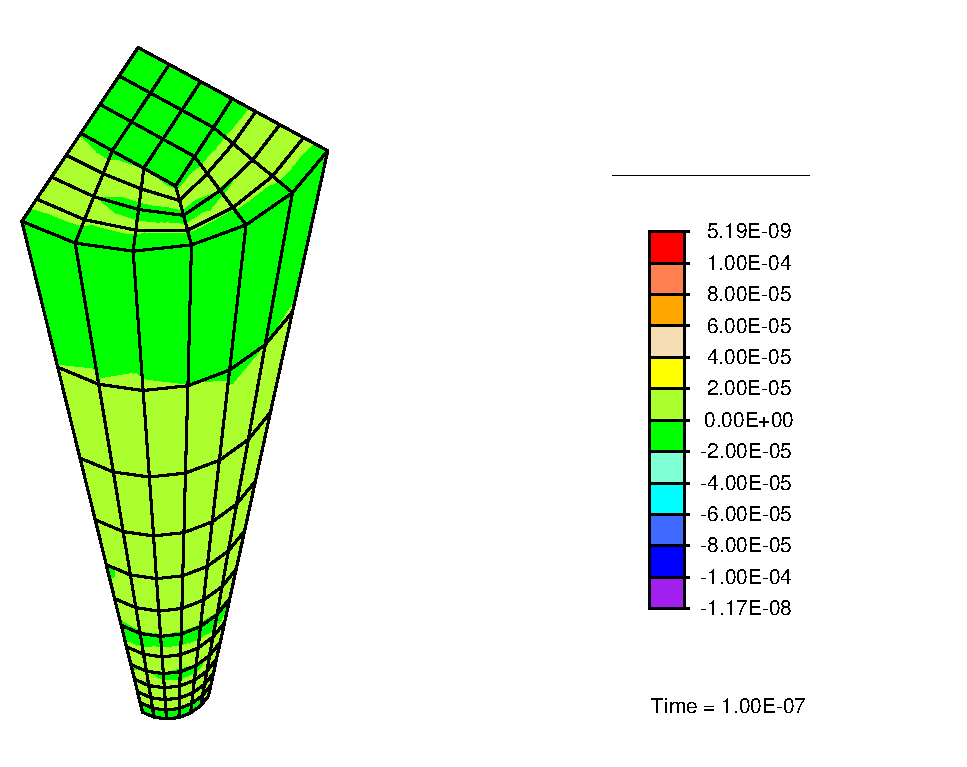
\includegraphics[width=7.5cm]{images/M5-100.eps}} \hskip 3cm (b)
\end{minipage}
\caption{Concentration gradient-driven flux
($\mathrm{kg.m}^{-2}\mathrm{sec}$) in the $\be_3$ direction at $1
\,\mathrm{nanosec.}$ and $100\,\mathrm{nanosec.}$ after the
beginning of loading. Note that the maximum and minimum values are
many orders of magnitude lower than for the other flux
contributions reported above. This is a demonstration of mechanics
influences dominating diffusion over the classical concentration
gradient contribution.} \label{M5fig}
\end{figure}

\begin{figure}[ht]
\begin{minipage}[t]{7.5cm}
{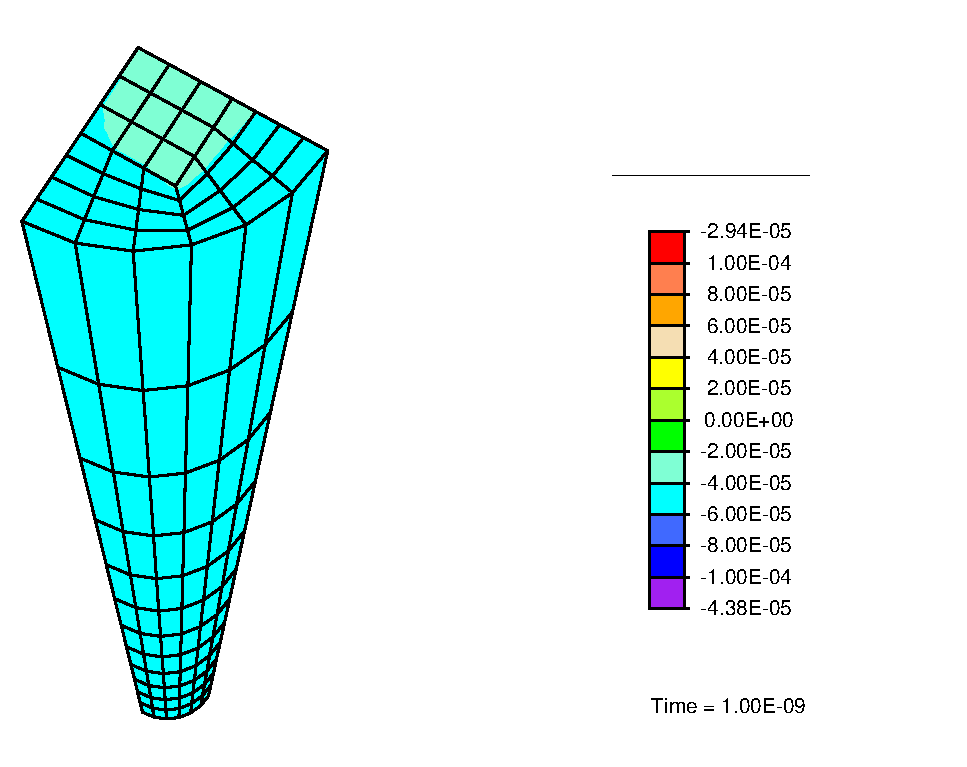
\includegraphics[width=7.5cm]{images/M-1.eps}} \hskip 3cm (a)
\end{minipage}
\begin{minipage}[t]{7.5cm}
{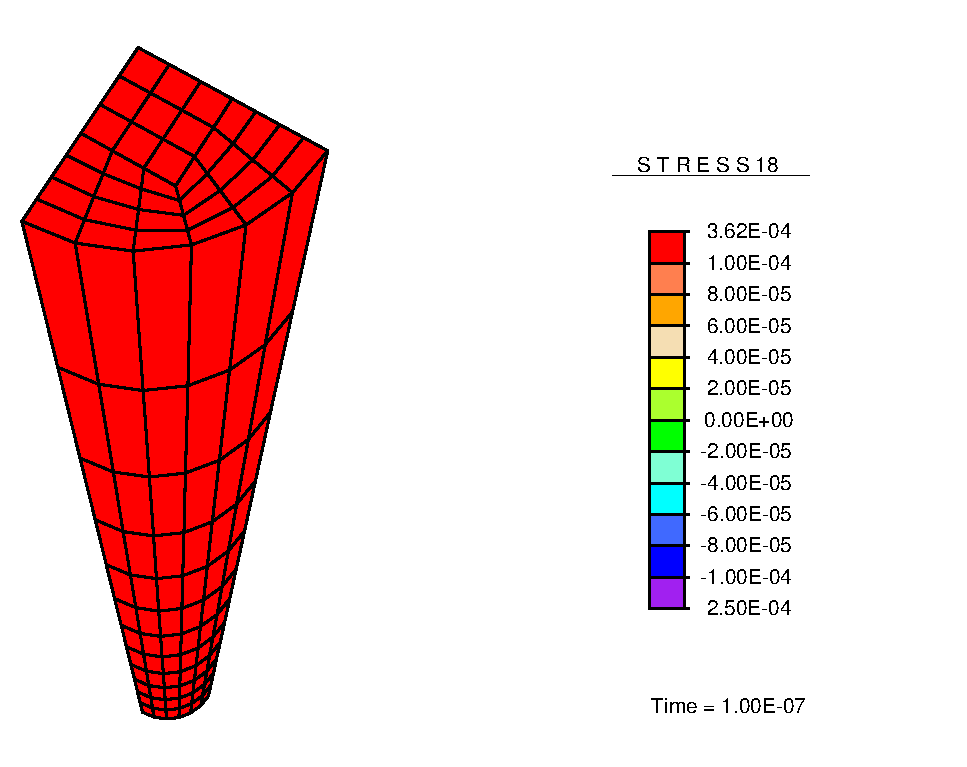
\includegraphics[width=7.5cm]{images/M-100.eps}} \hskip 3cm (b)
\end{minipage}
\caption{Total flux ($\mathrm{kg.m}^{-2}\mathrm{sec}$) in the
$\be_3$ direction at $1 \,\mathrm{nanosec.}$ and
$100\,\mathrm{nanosec.}$ after the beginning of loading. The
positive values indicate an upward flux, dominated by the stress
gradient driven contribution.} \label{Mfig}
\end{figure}

The flux contributions in Figures \ref{M1fig}--\ref{Mfig} can be
summarized as follows: The fluid flux is dominated by the
contribution from the stress gradient in the $\be_3$ direction.
The latter arises as the stress ($\sigma_{33}$) wave of tension
travels down the cylinder in the first few microseconds after
application of the load (the time taken to travel the length of
the cylinder is $12 \,\mu\mathrm{sec}$). Additionally, as the
fluid concentration changes due to the flux, it causes a further
change in the stress (Section \ref{sect5}). Other flux terms are
qualitatively sensible; i.e., their directions are consistent with
the physics of the problem, as argued in each of the figure
captions\footnote{In order to compare the flux contributions, they
have all been plotted on the same scale: $-1\times
10^{-4}--1\times 10^{-4} \,\mathrm{kg.m}^{-2}\mathrm{sec}$.
However the plots also show the maximum and minimum field values
at the top and bottom of the legend bars. These values represent a
better comparison of the relative flux magnitudes.}. There is some
loss of axial symmetry in a few of the plots due to the coarseness
of the finite element mesh for this example. It appears that
spatial oscillations in the solution lead to a further loss of
symmetry in Figures \ref{M2fig}b--\ref{M3fig}b and \ref{Mfig}a.
These oscillations arise due to large and dominant advective
terms, and need to be remedied by stabilized finite element
methods. Here, we only aim to demonstrate that various driving
forces for mass transport are in agreement with their theoretical
underpinnings in the paper. The resorption of the solid phase is
shown indirectly in Figure \ref{Pifig}. A positive fluid source,
$\Pi^\mathrm{f}$, means that $\Pi^\mathrm{s} < 0$. Since
$\Pi^\mathrm{s}$ is the only term balancing
$\partial\rho_0^\mathrm{s}/\partial t$ [see (\ref{massballocA})],
it follows that $\partial\rho_0^\mathrm{s}/\partial t < 0$.

\begin{figure}[ht]
\begin{minipage}[t]{7.5cm}
{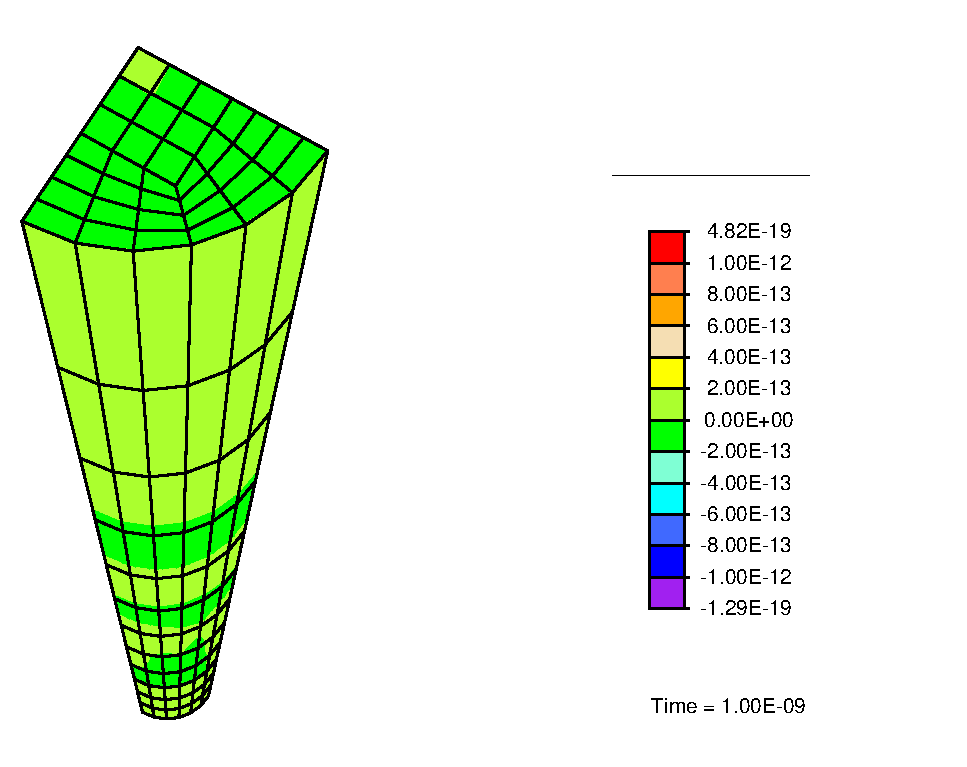
\includegraphics[width=7.5cm]{images/Pi-1.eps}} \hskip 3cm (a)
\end{minipage}
\begin{minipage}[t]{7.5cm}
{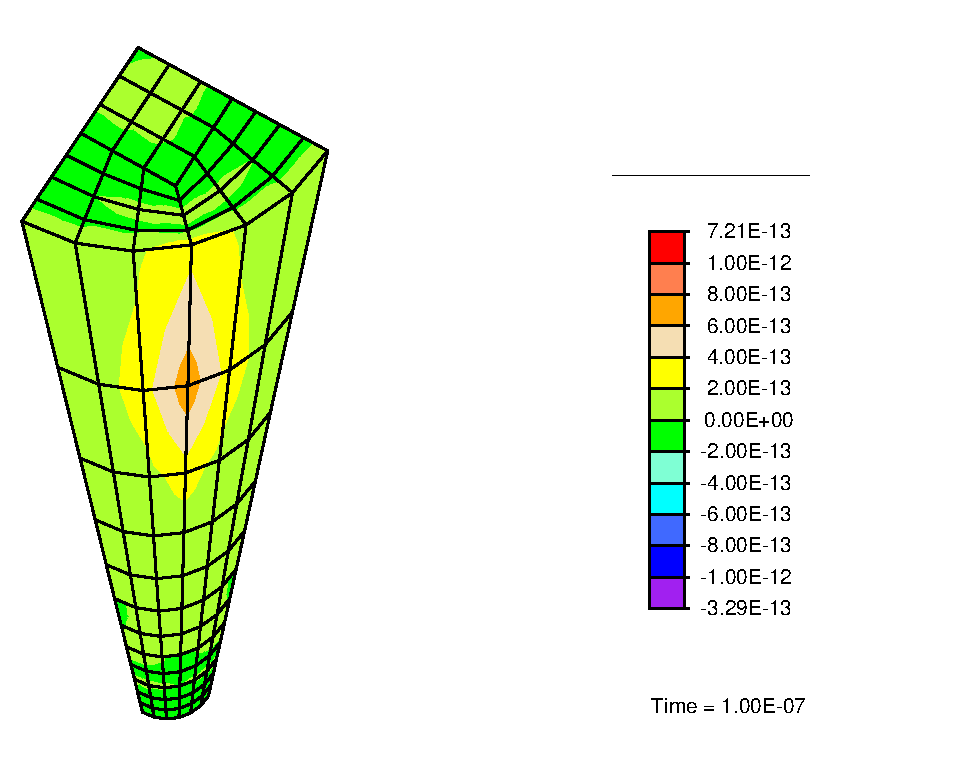
\includegraphics[width=7.5cm]{images/Pi-100.eps}} \hskip 3cm (b)
\end{minipage}
\caption{Rate of fluid production, $\Pi^\mathrm{f}$
($\mathrm{kg.m}^{-3}.\mathrm{sec}^{-1}$), at $1
\,\mathrm{nanosec.}$ and $100\,\mathrm{nanosec.}$ after the
beginning of loading. The positive values indicate that the local
fluid concentrations have fallen below their initial values.}
\label{Pifig}
\end{figure}

\section{Discussion and conclusions}
\label{sect7}

A general framework for growth of biological tissue has been
presented in this paper. While simplified models were used for
source terms, $(\Pi^\iota)$, they can be formulated on the basis
of the kinetics of chemical reactions in order to develop more
realistic growth laws. This approach, we believe, is fundamental
to a proper treatment of mass transport in tissue. Results are
obtained that differ fundamentally from the classical setting of
continuum mechanics. Most notable among these differences are the
mass fluxes driven by gradients in stress, strain, energy and
entropy, in addition to body force and inertia. Importantly,
though our treatment differs from classical mixture theory, the
two are fully consistent as established at several points in this
paper. The balance laws in Section \ref{sect2} and \ref{sect3}
introduce a degree of coupling between the phenomena of mass
transport and mechanics. This is visible most transparently in the
balance of linear momentum (\ref{ballinmomrefI}) that includes
mass fluxes, $\bM^\iota$. The balance of mass, described by
Equations (\ref{massballocA}) and (\ref{massballocI}), is also
dependent upon the mechanics as the discussion in Section
\ref{sect5.1} makes clear. Notably, this ensures
mechanics-mediated mass transport even with a mass source that is
independent of strain/stress, as the discussion at the end of
Section \ref{sect5.3} establishes. The discussion in Sections
\ref{sect5.1}--\ref{sect5.3} provides many insights into the
nature of this coupling. The mechanics problem also has a
constitutive dependence upon mass concentration, via
(\ref{stress-constrelI}) and the fact that the growth deformation
gradient tensor, $\bF^{\mathrm{g}^\iota}$ is determined by the
concentration. The viscoelastic nature of the composite tissue
would emerge naturally from a model incorporating a hyperelastic
solid and viscous fluid.

We have formally allowed all species to be load bearing and
develop a stress. At the scales that are of interest in a tissue,
the only relevant load bearing species are the solid and fluid
phases. Nevertheless, inasmuch as a transported species such as a
nutrient has a molecular structure that can be subject to loads at
the scale of pico-newtons, it is not inconsistent to speak of the
partial stress of this species. Since the constitutive relation
(\ref{stress-constrelI}) indicates that the partial stresses are
scaled by concentrations, the contribution to total stress from
any species besides the solid and fluid phases will be negligible.

We have chosen to leave remodelling out of our formulation in this
communication, to focus upon the above issues. Remodelling
includes any evolution in properties, state of stress, material
symmetry, volume or shape brought about by microstructural
changes. In the development of biological tissue, growth and
remodelling occur simultaneously. As density changes due to
growth, the material also remodels by microstructural evolution
within the neighborhood of each point. A rigorous treatment of
this phenomenon has been presented in the continuum mechanical
setting in a companion paper \citep{remodelpaper}.




\section{Balance equations and kinematics of growth}
\label{sec:2}

In this section, the coupled, continuum balance equations governing
the behaviour of growing tissue are summarised and specialised as
outlined in Section~\ref{sec:1}. For detailed continuum mechanical
arguments underlying the equations, the interested reader is directed
to \citet{growthpaper}.

The tissue of interest is an open subset of $\mathbb{R}^3$ with a
piecewise smooth boundary. At a reference placement of the tissue,
$\Omega_0$, points in the tissue are identified by their reference
positions, $\bX \in \Omega_0$. The motion of the tissue is a
sufficiently smooth bijective map $\Bvarphi: \overline{\Omega}_0
\times [0,T] \rightarrow \mathbb{R}^3$, where $\overline{\Omega}_0 :=
\Omega_0 \cup \partial\Omega_0$; $\partial\Omega_0$ being the boundary
of $\Omega_0$. At a typical time $t \in [0,T]$, $\Bvarphi(\bX,t)$ maps
a point $\bX$ to its current position, $\bx$. In its current
configuration, the tissue occupies a region $\Omega_t = \Bvarphi_t
(\Omega_0)$. These details are depicted in Figure~\ref{cp}. The
deformation gradient $\bF := \partial \Bvarphi/ \partial\bX$ is the
tangent map of $\Bvarphi$.

\begin{figure}[ht]
  \centering
  \psfrag{A}{\small$\bX$}
  \psfrag{F}{\small$\bx$}
  \psfrag{B}{\renewcommand{\baselinestretch}{1.5}\small$\Pi^\iota$}
  \psfrag{G}{\small$\pi^\iota$}
  \psfrag{E}{\small$\Bvarphi$}
  \psfrag{C}{\small$\Omega_0$}
  \psfrag{H}{\small$\Omega_t$}
  \psfrag{D}{\small$\bN\cdot\bM^\iota$}
  \psfrag{I}{\small$\bn\cdot\bm^\iota$}
	 {\includegraphics[width=10.00cm]{images/cp-mass-solute.eps}}
	 \caption{The tissue as a continuous medium with growing and
           diffusing species.}
	 \label{cp}
\end{figure}

The tissue consists of numerous species, of which the following
 groupings are of importance for the models: A solid species,
 consisting of solid \emph{collagen fibrils} and \emph{cells},\footnote{At this
 point, we do not distinguish the solid species further. This is a
 good approximation to the physiological setting for tendons, which
 are relatively acellular and whose dry mass consists of up to 75\%
 collagen \citep{Nordinetal:2001}.} denoted by $\mathrm{c}$, an
 extra-cellular \emph{fluid} species denoted by $\mathrm{f}$ and
 consisting primarily of water, and \emph{solute} species, consisting
 of precursors to reactions, byproducts, nutrients, and other
 regulatory chemicals. A generic solute will be denoted by
 $\mathrm{s}$. In what follows, an arbitrary species will be denoted
 by $\iota$, where $\iota = \mathrm{c,f,s}$.

The fundamental quantities of interest are mass concentrations,
$\rho_0^\iota(\bX,t)$. These are the masses of each species per unit
system volume in $\Omega_0$. Formally, these quantities can also be
thought of in terms of the maps $\rho_0^\iota: \overline{\Omega}_0
\times [0,T] \rightarrow \mathbb{R}$, upon which the formulation
imposes some smoothness requirements. By definition, the total {\em
material density} of the tissue at a point is a sum of these
concentrations over all species $\sum\limits_{\iota}\rho_0^\iota =
\rho_0$. Other than the solid species, $\mathrm{c}$, all phases have
mass fluxes, $\bM^\iota$.\footnote{Currently, we do not consider
  certain physiological 
processes, such as the migration of fibroblasts within the
extra-cellular matrix during wound healing, which may otherwise be
modelled as mass transport.} These are mass flow rates per unit
cross-sectional area in the reference configuration \emph{defined
relative to the solid phase}. The species have mass sources (or
sinks), $\Pi^\iota$.

\subsection{Balance of mass for an open system}
\label{bomass} As a result of mass transport (via the flux terms) and
inter-conversion of species (via the source/sink terms) introduced
above, the concentrations, $\rho_0^\iota$, change with time. In
local form, the balance of mass for an arbitrary species in the
reference configuration is

\begin{equation}
\frac{\partial\rho_0^\iota}{\partial t} = \Pi^\iota -
\mathrm{\small{DIV}}[\bM^\iota],\;\forall\,\iota,
\label{massbalance1}
\end{equation}

\noindent recalling that, in particular, $\bM^{c} = \bzero$. Here,
$\mathrm{\small{DIV}[\bullet]}$ is the divergence 
operator in the reference configuration. The functional forms of
$\Pi^\iota$ are abstractions of the underlying biochemistry,
physiologically relevant examples of which are discussed in
Section~\ref{sources}, and the fluxes, $\bM^\iota$, are determined
from the thermodynamically-motivated constitutive relations described
in Section~\ref{flux const}.

The behaviour of the entire system can be determined by summing
\mbox{Equation~(\ref{massbalance1})} over all species $\iota$.
Additionally, sources and sinks satisfy the relation

\begin{equation}
\sum\limits_\iota\Pi^\iota = 0, \label{sourcebalance}
\end{equation}

\noindent which is consistent \citep{growthpaper} with the Law of Mass
Action for reaction rates and with Mixture Theory
\citep{TruesdellNoll:65}.

\subsubsection{The role of mass balance in the current
configuration}\label{curr-ref-mb}



In order to proceed, we must first introduce the central kinematic
assumption underlying the 
formulation: We assume that the pore structure deforms with the
collagenous phase. Therefore, the deformation gradient, $\bF$, is
common to c and the fluid-filled pore spaces. Furthermore, in what
follows, we will treat the fluid as ideal and nearly-incompressible,
i.e. as elastic (Section \ref{compfluid}). This combination of
kinematic and constitutive assumptions to be elaborated upon, implies
that the stress in the fluid phase is determined by the elastic part of
$\bF$ (see Sections \ref{growthkinem} and
\ref{compfluid}). For clarity we denote it as
$\bF^{\mathrm{e}^\mathrm{f}}$. Importantly, the pore-filling fluid under stress
can also undergo transport relative to the pore network; i.e.,
relative to the collagenous phase. This is the fluid flux, denoted by
$\bM^\mathrm{f}$ in the reference configuration. Note that the
specification of constitutive relations for the flux is still open at
this point in the discussion. At the outset, we preclude stress in any
of the solute species, s. Only the solid collagen and fluid bear
stress. 

Although the initial/boundary value problem of mass transport can be
consistently posed in the reference configuration, the evolving
current configuration, $\Omega_t$, is of greater interest from a
physical standpoint for growth problems. It follows from the
discussion in the preceding paragraph that the shape and size of
pores in $\Omega_t$ is determined by $\bF$. Therefore, at
the boundary, the fluid concentration with 
respect to $\Omega_t$ remains constant if the boundary is in contact
with a fluid bath.  Accordingly, this is the appropriate Dirichlet
boundary condition to impose under normal physiological
conditions. This is shown in an idealised manner in Figure~\ref{fbc}.

\begin{figure}
\centering
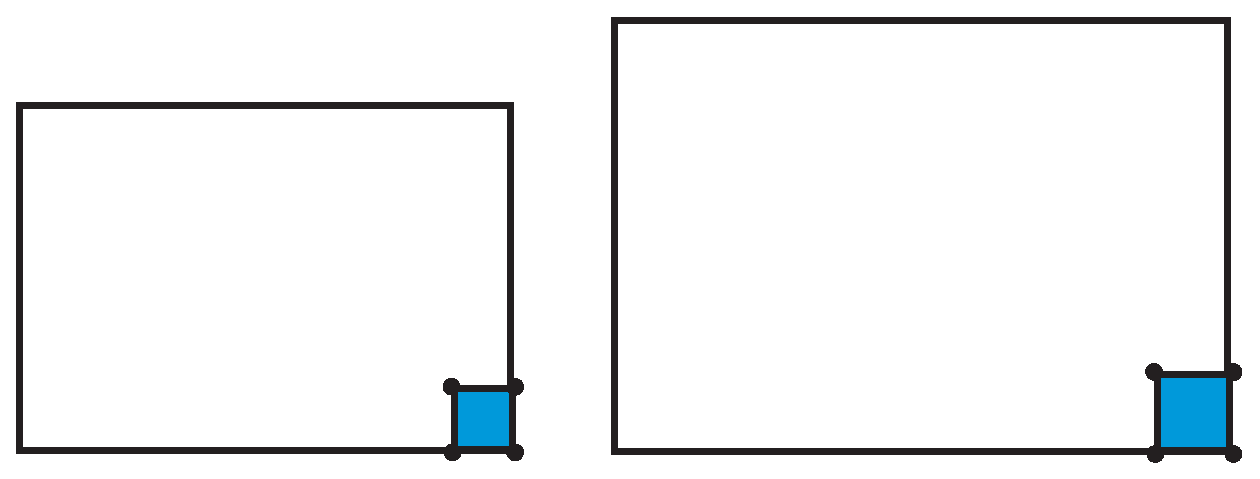
\includegraphics[width=10.00cm]{images/concentration.eps}
\caption{If the pore structure at the boundary deforms with the
tissue and this boundary is in contact with a fluid bath, the
fluid concentration with respect to the current configuration,
i.e., $\rho^\mathrm{f}$, remains constant.}\label{fbc}
\end{figure}

In the interest of applying boundary conditions (either specification
of species flux or concentration) that are physically meaningful, we
use the local form of the balance of mass in the current
configuration,

\begin{equation}
\frac{\mathrm{d}\rho^\iota}{\mathrm{d}t} = \pi^\iota-
\mathrm{\small{div}}[\bm^\iota] - \rho^\iota
\mathrm{\small{div}}[\bv],\;\forall\,\iota, \label{massbalcurr}
\end{equation}

\noindent where $\rho^\iota(\bx,t),\pi^\iota(\bx,t)$, and
$\bm^\iota(\bx,t)$ are the current mass concentration, source and mass
flux of species $\iota$ respectively and $\bv(\bx,t)$ is the velocity
of the solid phase. They are related to corresponding reference
quantities as $\rho^\iota = \left(\mathrm{det} \left(\bF\right)
\right)^{-1} \rho_0^\iota$, $\pi^\iota = \left(\mathrm{det}
\left(\bF\right) \right)^{-1} \Pi^\iota$ and $\bm^\iota =
\left(\mathrm{det} \left(\bF\right) \right)^{-1} \bF \bM^\iota$. The
spatial divergence operator is $\mbox{\small{div} [\textbullet]}$, and
the left hand-side in Equation~(\ref{massbalcurr}) is the material
time derivative relative to the solid, which may be written explicitly as
$\frac{\partial}{\partial t}\vert_X$, implying that the reference
position of the solid collagenous skeleton is held fixed.

\subsection{The kinematics of growth induced by changes in concentration}
\label{growthkinem}

\begin{figure}[ht]
  \centering
  \psfrag{A}{\small $\Omega_0$}
  \psfrag{B}{\small $\Omega^\ast$}
  \psfrag{C}{\small $\Omega_t$}
  \psfrag{D}{\small $\bX$}
  \psfrag{E}{\small $\bX^\ast$}
  \psfrag{F}{\small $\bx$}
  \psfrag{G}{\small $\bF^{\mathrm{g}^{\mathrm{\iota}}}$}
  \psfrag{H}{\small $\widetilde{\bF}^{\mathrm{e}^{\mathrm{\iota}}}$}
  \psfrag{I}{\small $\widetilde{\bF}$}
  \psfrag{J}{\small $\overline{\bF}^\mathrm{e}$}
  \psfrag{K}{\small $\bF$}
  \psfrag{L}{\small $\Bkappa$}
  \psfrag{M}{\small $\bu^\ast$}
  \psfrag{N}{\small $\Bvarphi$}
         {\includegraphics[width=10.00cm]{images/kinematics.eps}}
     \caption{The kinematics of growth, which holds for $\iota =
     \mathrm{c,f}$.} 
     \label{growthkine}
\end{figure}

Local volumetric changes are associated with changes in the
concentrations of the solid collagen and fluid, $\iota =
     \mathrm{c,f}$. If the material of the solid collagen or fluid remains
stress free, it swells with an
increase in concentration (mass of the species per unit system
volume), and shrinks as its concentration decreases. This leads to the
notion of a \emph{growth deformation gradient}. One aspect of the
coupling between mass transport and mechanics stems from this
phenomenon. In the setting of finite strain kinematics, the total
deformation gradient, $\bF$, is decomposed into the growth component
of the solid collagen, $\bF^{\mathrm{g}^\mathrm{c}}$, a
\emph{geometrically-necessitated elastic component} 
accompanying growth, $\widetilde{\bF}^{\mathrm{e}^\mathrm{c}}$ and an \emph{additional elastic component due
to external stress}, $\overline{\bF}^{\mathrm{e}^\mathrm{c}}$. Later,
we will write $\bF^{\mathrm{e}^\mathrm{c}} =
\overline{\bF}^{\mathrm{e}^\mathrm{c}}\widetilde{\bF}^{\mathrm{e}^\mathrm{c}}$.
This split is analogous to the classical
decomposition of multiplicative plasticity \citep{Lee:69} and is
similar to the approach followed in existing literature on biological
growth \citep[see for
  e.g.][]{Klischetal:2001,TaberHumphrey:2001,AmbrosiMollica:2002}. As
explained in Section \ref{curr-ref-mb}, we assume that the
fluid-filled pores also deform with $\bF$, and that a component,
$\bF^{\mathrm{e}^\mathrm{f}}$, of this total deformation gradient
tensor, determines the fluid stress. We also assume a fluid growth
component, $\bF^{\mathrm{g}^\mathrm{f}}$, which we elaborate below,
and that $\bF^{\mathrm{e}^\mathrm{f}}\bF^{\mathrm{g}^\mathrm{f}} =
\bF$. As with the solid collagen we admit $\bF^{\mathrm{e}^\mathrm{f}}
=
\overline{\bF}^{\mathrm{e}^\mathrm{f}}\widetilde{\bF}^{\mathrm{e}^\mathrm{f}}$,
the sub-components carrying the same interpretation as for the solid
collagen. However, we do not explicitly use this last decomposition.

The elastic-growth decomposition is visualised in \mbox{Figure~\ref{growthkine}}.
Assuming that the volume changes associated with growth described
above are isotropic, a simple form for the growth part of the
deformation gradient tensor is

\begin{equation}
\bF^{\mathrm{g}^\iota} = \left(
  \frac{\rho_0^\iota}{\rho_{0_{\mathrm{ini}}}^\iota} \right)^
  {\frac{1}{3}} 
{\bf 1},\quad \iota = \mathrm{c,f}
\label{isotropicgrowth} 
\end{equation} 

\noindent where
$\rho_{0_{\mathrm{ini}}}^\iota(\bX)$ is the reference concentration at the
initial time, and {\bf 1} is the second-order isotropic
tensor.\footnote{This choice is only the simplest possible. Given the
  highly directional micro-structure and mechanical properties of many
  tissues, it seems likely that anisotropic growth is actually 
  more common. Wolff's Law for bone growth is one example. This is a
  topic of ongoing investigation, and one that we will report on in
  greater detail in a future communication.} In 
the state, $\bF = \bF^{\mathrm{g}^\iota}$, the species would be stress
free. The kinematics being local, the
action of $\bF^{\mathrm{g}^\iota}$ alone can result in
incompatibility, which is eliminated by the geometrically-necessary
elastic deformation
$\widetilde{\bF}^{\mathrm{e}^{\mathrm{\iota}}}$, which causes an
internal, self-equilibrated stress. The component
$\overline{\bF}^{\mathrm{e}^\iota}$ is associated with the external stress.

\subsubsection{Saturation and tissue swelling}\label{satswel}

\begin{figure}[ht]
\centering 
  \psfrag{A}{\small A}
  \psfrag{B}{\small B}
  \psfrag{C}{\small B}
  \psfrag{D}{\small C}
  \psfrag{E}{\small Unsaturated}
  \psfrag{F}{\small Saturated}
{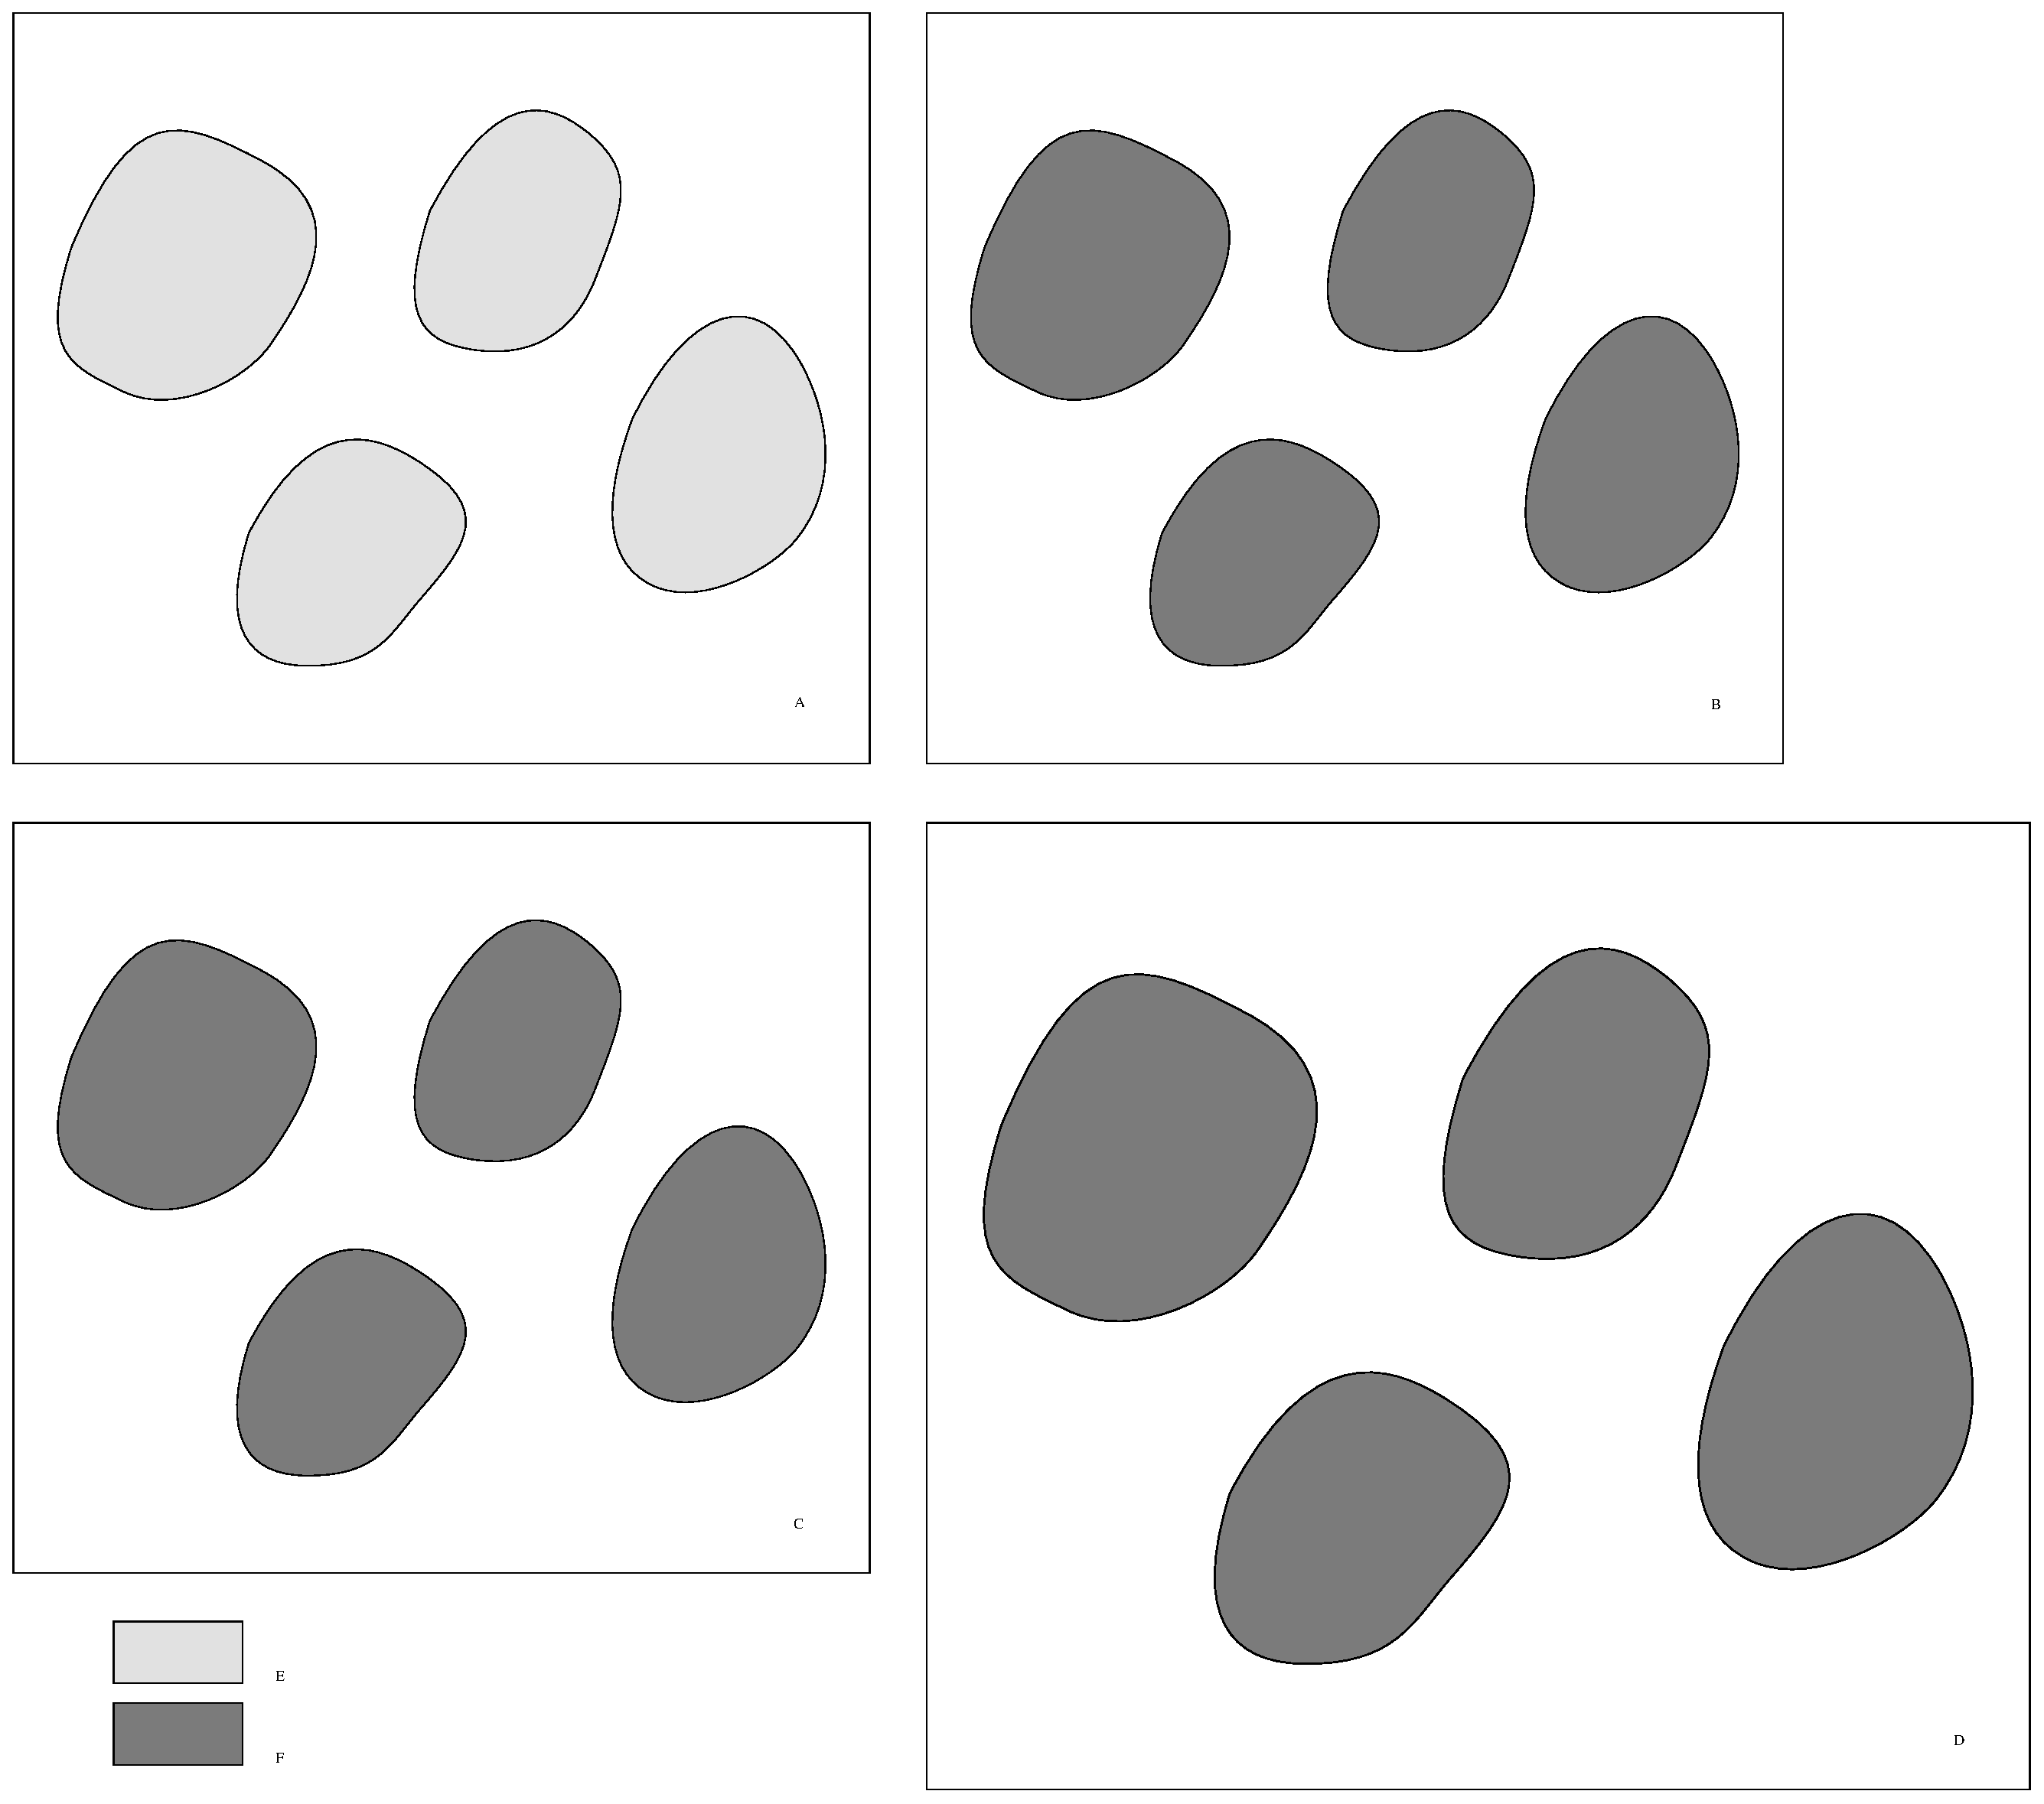
\includegraphics[width=10.00cm]{images/composite.eps}}

\caption{Unsaturated tissue in the current configuration (A) allows
  influx of fluid 
  without swelling until it is completely saturated (B). Initially
  saturated tissue (B), in general, swells with influx of fluid (C).}

\label{satswelfig}
\end{figure}

\noindent The degree of saturation of the solid phase plays a
fundamental role in determining whether the tissue responds to an
infusion (expulsion) of fluid by swelling (shrinking). In 
particular, the isotropic swelling law defined by Equation
(\ref{isotropicgrowth}) has to be generalised to treat the case in
which the solid phase is not saturated by fluid.

Figure~\ref{satswelfig} schematically depicts two possible
scenarios. If the tissue is unsaturated in its current configuration,
as in A, then, on a microscopic scale, it 
contains unfilled voids. It is thus capable of allowing an influx of
fluid, which tends to increase its degree of saturation until fully
saturated, as in  B. This increase 
does not cause swelling of the tissue in the local stress-free state, as
there is free volume for 
incoming fluid to occupy. However, once the tissue is
saturated in the current configuration, an increase in the
fluid content causes swelling in the stress-free state, as depicted in
C, since there is no free volume for the 
entering fluid to occupy. It is this second case that is modelled by
(\ref{isotropicgrowth}). It is worth emphasizing that this argument
holds for $\bF^{\mathrm{g}^\mathrm{f}}$, which is the local
stress-free state of deformation of the fluid-containing pores at a point. The
actual deformation gradient, $\bF =
\bF^{\mathrm{e}^\mathrm{f}}\bF^{\mathrm{g}^\mathrm{f}}$, also depends
on the the elastic part, $\bF^{\mathrm{e}^\mathrm{f}}$, which is
determined by the constitutive response of the fluid. Under stress, an
incompressible fluid will have
$\mathrm{det}\bF^{\mathrm{e}^\mathrm{f}} = 1$ and therefore a
fluid-saturated tissue will swell with fluid influx, $\mathrm{det}\bF
= \mathrm{det}\bF^{\mathrm{g}^\mathrm{f}} > 1$. A compressible fluid
may have $\mathrm{det}\bF^{\mathrm{e}^\mathrm{f}} < 1$ allowing
$\mathrm{det}\bF < 1$ even with
$\mathrm{det}\bF^{\mathrm{g}^\mathrm{f}} >1$. Even in this case,
however, in the stress-free state there will be swelling.

Therefore, for the fluid phase, the isotropic swelling law can be
extended to the unsaturated case by 
introducing a degree of saturation, $\tilde{v}^\iota$, defined in the
current configuration, $\Omega_t$. We have $\tilde{v}^\iota =
\rho^\iota/\tilde{\rho}^\iota$, where 
$\tilde{\rho}^\iota$ is the intrinsic density in $\Omega_t$ and is
given by $\tilde{\rho}^\iota =
\tilde{\rho}^\iota_0/\mathrm{det}\bF$. Note that the intrinsic
reference density, $\tilde{\rho}^\iota_0$, is a material property. Upon
solution of the 
mass balance equation (\ref{massbalcurr}) for $\rho^\iota$, the
species volume fractions, $\tilde{v}^\iota$, can therefore be computed
in a straightforward fashion. The sum of these
volume fractions is our required measure of saturation defined in
$\Omega_t$. Also, recognizing
that for the dilute solutions obtained with
physiologically-relevant solute concentrations, the saturation
condition is very well approximated by $\tilde{v}^\mathrm{f} +
\tilde{v}^\mathrm{s} = 1$, we proceed to
redefine the fluid growth-induced component of the pore deformation gradient
tensor as follows:

\begin{equation}
\bF^{\mathrm{g}^\mathrm{f}} = \left\{ \begin{array}{ll}  \left(
\frac{\rho_0^\mathrm{f}}{\rho_{0_{\mathrm{sat}}}^\mathrm{f}} \right)^
{\frac{1}{3}}{\bf 1},&
\tilde{v}^\mathrm{f} + \tilde{v}^\mathrm{s} = 1 \\ {\bf 1},& \mathrm{otherwise.}
\end{array}\right.
\label{saturation}
\end{equation}

\noindent In (\ref{saturation}) $\rho_{0_{\mathrm{sat}}}^\mathrm{f}$
is the reference concentration value at which the tissue attains saturation
in the current configuration.

With this redefinition of $\bF^{\mathrm{g}^\mathrm{f}}$ it is implicit
that $\tilde{v}^\mathrm{f} + \tilde{v}^\mathrm{s} > 1$ is
non-physical. Saturation holds in the sense that $\tilde{v}^\mathrm{f} +
\tilde{v}^\mathrm{s} = 1$, and it actually allows $\sum_\iota
\tilde{v}^\iota > 1$ if the sum is over all species. It has been
common in the soft tissue literature to assume that, 
under normal physiological 
conditions, soft tissues are fully saturated by the fluid and
\mbox{Equation~(\ref{isotropicgrowth})} is appropriate for $\iota =
\mathrm{f}$. However, this treatment of saturation and swelling
induced by the fluid phase is necessary background for Section
\ref{tensionfluid} where we 
discuss the response of the fluid phase under tension. This treatment
also holds relevance for partial drying,
which \emph{ex vivo} or \emph{in vitro} tissue may be subject to under
certain laboratory conditions, and is central to the mechanics of
drained porous media other than biological tissue, most prominently,
soils. 

\subsection{Balance of momenta}
\label{bomom}

In soft tissues, the species production rate and flux that appear on
the right hand-side in Equations~(\ref{massbalance1}) and
(\ref{massbalcurr}), are strongly 
dependent on the local state of stress. To correctly model this
coupling, the balance of linear momentum should be solved to determine
the local state of strain and stress.

The deformation of the tissue is characterised by the map
$\Bvarphi(\bX,t)$. Recognising that, in tendons, the solid collagen
fibrils and fibroblasts do not undergo mass
transport, the material velocity of this species, $\bV =
\partial\Bvarphi/\partial t$, is used as the primitive variable for
mechanics. Each remaining species can undergo mass transport relative
to the solid collagen. For this purpose, it is useful to define the
material velocity of a 
species $\iota$ \emph{relative to the solid skeleton} as: $\bV^\iota =
(1/\rho_0^\iota)\bF\bM^\iota$. Thus, the total material velocity of a
species $\iota$ is $\bV+\bV^\iota$.

The total first Piola-Kirchhoff stress tensor, $\bP$, is the sum of
the partial stresses $\bP^{\,\iota}$ (borne by a species $\iota$) over all
the species present. Recognizing that solutes in low concentrations,
and do not bear 
  appreciable stress, the partial stresses and momentum balance
  equation are defined only for the solid collagen and fluid
  phases. With the introduction 
  of these quantities, the 
balance of linear momentum in local form over $\Omega_0$ for solid
collagen and fluid is,

\begin{equation}
\begin{split}
\rho_0^\iota\frac{\partial}{\partial t}\left(\bV+\bV^\iota\right) &
=\rho^\iota_0\left(\bg+\bq^\iota\right) +
\mathrm{\small{DIV}}[\bP^{\,\iota}]\\ 
& \quad -\left(\mathrm{\small{GRAD}}\left[\bV+
  \bV^\iota\right]\right)\bM^\iota, \quad \iota = \mathrm{c,f}
\label{linearmombalance}
\end{split}
\end{equation} 

\noindent where $\bg$ is the body force per unit mass, and $\bq^\iota$
is an interaction term denoting the force per unit mass exerted upon
$\iota$ by all other species present. The final term with the
(reference) gradient denotes the contribution of the flux to the
balance of momentum. In practise, the relative magnitude of the fluid
mobility (and hence flux) is small, so the final term on the right
hand side of Equation~(\ref{linearmombalance}) is negligible,
resulting in a more classical form of the balance of
momentum. Furthermore, in the absence of significant acceleration of
the tissue during growth, the left hand-side can also be neglected,
reducing (\ref{linearmombalance}) to the quasi-static balance of
linear momentum.

The balance of momentum of the entire tissue is obtained by summing
Equation~(\ref{linearmombalance}) over $\iota = \mathrm{c,f}$. Additionally,
recognising that the rate of change of momentum of the entire tissue
is affected only by external agents and is independent of internal
interactions, the following relation arises.

\begin{equation}
\sum\limits_{\iota =
  \mathrm{c}}^\mathrm{f}\left(\rho^\iota_0\bq^\iota+\Pi^\iota
\bV^\iota 
\right)= 0. \label{qrelation}
\end{equation}

\noindent This is also consistent with Classical Mixture Theory
\citep{TruesdellNoll:65}. See \citet{growthpaper} for further
details on balance of linear momentum, and the formulation of
balance of angular momentum. We only note here that the latter
principle leads to a symmetric partial Cauchy stress,
$\Bsigma^\iota$ for each species in contrast with the unsymmetric
Cauchy stress of \cite{EpsteinMaugin:2000}.

\section{Constitutive framework and specific models}
\label{sec:3}

As is customary in field theories of continuum physics, the
Clausius-Duhem inequality is obtained by multiplying the Entropy
Inequality (the Second Law of Thermodynamics) by the temperature
field, $\theta$, and subtracting it from the Balance of Energy (the
First Law of Thermodynamics). We assume the Helmholtz free energy per
unit mass of species $\iota$ to have the form:\footnote{Conceivably,
  the mass-specific Helmholtz free energy of one species could be a function of the
  concentration of other species. Ion concentrations, for instance,
  can determine the state of osmotic tension of certain soft
  tissues. Therefore, this choice represents a 
  constitutive restriction.}
$\psi^{\iota} = \hat{\psi}^\iota(\bF^{\mathrm{e}^\iota},
\theta, \rho_0^\iota)$.  Substituting this in the Clausius-Duhem
inequality results in a form of this inequality that the specified
constitutive relations \emph{must not} violate. Only the valid
constitutive laws relevant to the examples that follow are listed
here. For details, see \cite{growthpaper}.

\subsection{An anisotropic network model based on entropic
elasticity}\label{wlcm}


The partial first Piola-Kirchhoff stress of collagen, modelled as a
hyperelastic material, is $\bP^{\,\mathrm{c}} = \rho_0^\mathrm{c} \partial
\psi^\mathrm{c}/ \partial\bF^{\mathrm{e}^\mathrm{c}}$. Recall that
$\bF^{\mathrm{e}^\mathrm{c}} = \bF\bF^{\mathrm{g}^{\mathrm{c}^{-1}}}$
is the elastic part, and
$\bF^{\mathrm{g}^\mathrm{c}}$ 
is the growth part, respectively, of the deformation gradient, of
collagen. Following Equation 
(\ref{isotropicgrowth}), if we were considering unidirectional growth
of collagen along a unit vector $\be$, we would have
$\bF^{\mathrm{g}^\mathrm{c}} = \frac{\rho^\mathrm{c}_{0}}
{\rho^\mathrm{c}_{0_{\mathrm{ini}}}} \be \otimes \be$, with
$\rho^\mathrm{c}_{0_{\mathrm{ini}}}$ denoting the initial
concentration of collagen at the point.

The mechanical response of tendons in tension is determined primarily
by their dominant structural component: highly oriented fibrils of
collagen. In our preliminary formulation, the strain energy density
for collagen has been obtained from hierarchical multi-scale
considerations based upon an entropic elasticity-based worm-like chain
(WLC) model \citep{KratkyPorod:49}. The WLC model has been widely used
for long chain single molecules, most prominently for DNA
\citep{MarkoSiggia:95,Riefetal:97,Bustamanteetal:2003}, and recently
for the collagen mono\-mer \citep{Sunetal:2002}. The central
parameters of this model are the chain's contour length, $L$, and
persistence length, $A$. The latter is a measure of its stiffness and
given by $A = \chi/k\theta$, where $\chi$ is the bending rigidity, $k$
is Boltzmann's constant and $\theta$ is the temperature. See
\citet{LandLif} for general formulation of statistical mechanics
models of long chain molecules. 

To model a collagen network structure, the
WLC model has been embedded as a single constituent chain of an
eight-chain model \citep{Bischoffetal:2002, Bischoffetal1:2002},
depicted in \mbox{Figure~\ref{eightchain}}.  Homogenisation via
averaging then leads to a continuum Helmholtz free energy function,
$\hat{\psi}^\mathrm{c}$:\footnote{Under the isothermal conditions
  assumed here, $\hat{\psi}^\mathrm{c}$ is independent of
  $\theta$ in the 
  strain energy. Accordingly, we have the parametrisation
  ${\psi}^\mathrm{c}=\hat{\psi}^\mathrm{c}
  (\bF^{\mathrm{e}^\mathrm{c}},\rho^\mathrm{c}_{0})$ .}

\begin{equation}
\begin{split}
\rho^\mathrm{c}_{0}\hat{\psi}^\mathrm{c} (\bF^{\mathrm{e}^\mathrm{c}},\rho^\mathrm{c}_{0})
&= \frac{N k \theta}{4 A}\left(\frac{r^2}{2L} + \frac{L}{4(1-r/L)} -
\frac{r}{4}\right)\\ & +
\frac{\gamma}{\beta}({J^{\mathrm{e}^{\mathrm{c}^{-2\beta}}}} -1) +
\gamma{\bf 1}\colon(\bC^{\mathrm{e}^{\mathrm{c}}}-{\bf 1})\\ &-\frac{N
k \theta}{4\sqrt{2L/A}}\left(\sqrt{\frac{2A}{L}} + \frac{1}{4(1 -
\sqrt{2A/L})} -\frac{1}{4} \right) Z,\\ Z &=
\log\left(\lambda_1^{{\mathrm{e}}^{a^\mathrm{2}}}
\lambda_2^{{\mathrm{e}}^{b^\mathrm{2}}}
\lambda_3^{{\mathrm{e}}^{c^\mathrm{2}}}\right).
\label{wlcmeq}
\end{split}
\end{equation}

Here, $N$ is
the density of chains, and $a,b$ and $c$ are lengths of the unit cell
sides aligned with the principal stretch directions. The material
model is isotropic only if $a=b=c$.

\begin{figure}
\psfrag{r}{\small $r$}
\psfrag{A}{\small $A$}
\psfrag{a}{\small $a$}
\psfrag{b}{\small $b$}
\psfrag{c}{\small $c$}
\psfrag{n}{\small$\bN_1$}
\psfrag{o}{\small$\bN_2$}
\psfrag{p}{\small$\bN_3$}
\centering {\includegraphics[width=10.00cm]{images/wlcm-cuboid.eps}}
\caption{\small The eight-chain model incorporating worm-like
  chains.}\label{eightchain}
\end{figure}

The elastic stretches along the unit cell axes are, respectively,
denoted by
$\lambda_1^{\mathrm{e}},
\lambda_2^{\mathrm{e}}$ 
and 
$\lambda_3^{\mathrm{e}}$, $\bC^{\mathrm{e}^{\mathrm{c}}} =
\bF^{\mathrm{e}^{\mathrm{c}^{\mathrm{T}}}}
\bF^{\mathrm{e}^{\mathrm{c}}}$ is the elastic right Cauchy-Green
tensor of collagen. The factors $\gamma$ and $\beta$ control
the bulk compressibility of the model. The end to end chain length is
given by $r = \frac{1}{2}\sqrt{a^2\lambda_1^{\mathrm{e}^2} +
  b^2\lambda_2^{\mathrm{e}^2}+c^2\lambda_3^{\mathrm{e}^2}}$, where
$\lambda^\mathrm{e}_I = 
\sqrt{\bN_I\cdot\bC^{\mathrm{e}^{\mathrm{c}}}\bN_I}$, and $\bN_I,\,I =
1,2,3$ are the unit vectors along the three unit cell axes,
respectively. In our numerical simulations that appear below in
Section~\ref{numericalimplementation}, the numerical values used for
the parameters introduced in (\ref{wlcmeq}) are based on those in
\citet{kuhlremod05}.

\subsection{A nearly incompressible ideal fluid}
\label{compfluid}

In this preliminary work, the fluid phase is treated as nearly
incompressible and ideal, i.e., inviscid. The partial Cauchy
stress in the fluid is
\begin{equation}
\Bsigma^\mathrm{f} =
\mathrm{det}(\bF^{\mathrm{e}^\mathrm{f}})^{-1}
\bP^{\,\mathrm{f}}\bF^{\mathrm{e}^\mathrm{fT}} 
= h(\rho^\mathrm{f}){\bf 1},\label{Pf}
\end{equation}

\noindent where a large value of $h^\prime(\rho^\mathrm{f})$ ensures
near-in\-comp\-ress\-i\-bil\-i\-ty. 
 
\subsubsection{Response of the fluid in tension;
cavitation}\label{tensionfluid}

The response of the ideal fluid, as defined by \mbox{Equation
  (\ref{Pf})}, does not distinguish between tension and compression,
  i.e., whether 
$\mathrm{det}(\bF^{\mathrm{e}^\mathrm{f}}) \gtreqless 1$. Being
(nearly) incompressible, the fluid can develop compressive hydrostatic
  stress
without bound---a case that is modelled accurately. However, the fluid
can develop at most a small tensile hydrostatic stress
\citep{cavitationchris},\footnote{Where, we are referring to the fluid
  being subject to net tension, not a reduction in fluid compressive
  stress from reference ambient pressure.} and the tensile
stiffness is mainly from the collagen phase. This is not accurately
represented by (\ref{Pf}), which models a symmetric response in
tension and compression.

Here, we preclude all tensile load carrying by the fluid by limiting
$\mathrm{det}(\bF^{\mathrm{e}^\mathrm{f}}) \leq 1$. We first introduce
an additional component to the relation between 
deformation of the pore space, given by $\bF$, the fluid
stress-determining tensor, 
$\bF^{\mathrm{e}^\mathrm{f}}$ and the growth tensor for the fluid,
$\bF^{\mathrm{g}^\mathrm{f}}$. Consider the cavitation (void forming) tensor,
$\bF^{\mathrm{v}}$, defined by
  
\begin{equation}
 \bF^{\mathrm{e}^\mathrm{f}}\bF^{\mathrm{g}^\mathrm{f}}
 \bF^{\mathrm{v}} = \bF.
\label{fvoid}
\end{equation}


We restrict the formulation to include only saturated current
configurations at $t = 0$. Following Section \ref{satswel} we have
$\tilde{v}^\mathrm{f} + \tilde{v}^\mathrm{c} = 1$ at $t = 0$, the saturation
condition in $\Omega_t$ when solutes are at low
concentrations. At times $t > 0$ Equation (\ref{saturation}) holds for
$\bF^{\mathrm{g}^\mathrm{f}}$. If
$\mathrm{det}[\bF(\bF^{\mathrm{g}^\mathrm{f}})^{-1}] \le 1$ we set
$\bF^{\mathrm{e}^\mathrm{f}} = \bF(\bF^{\mathrm{g}^\mathrm{f}})^{-1}$
and $\bF^{\mathrm{v}} = {\bf 1}$ for no cavitation. Otherwise, since
$\mathrm{det}[\bF(\bF^{\mathrm{g}^\mathrm{f}})^{-1}] > 1$, we specify
$\bF^{\mathrm{e}^\mathrm{f}} =
\mathrm{det}[\bF(\bF^{\mathrm{g}^\mathrm{f}})^{-1}]^{-1/3}\bF(\bF^{\mathrm{g}^\mathrm{f}})^{-1}$
thus restricting
$\bF^{\mathrm{e}^\mathrm{f}}$ to be unimodular and allow cavitation by
writing $\bF^{\mathrm{v}} = \bF(\bF^{\mathrm{e}^\mathrm{f}}\bF^{\mathrm{g}^\mathrm{f}})^{-1}$.
These conditional relations are summarized as 

\begin{equation}
\bF^{\mathrm{e}^\mathrm{f}} = \left\{ \begin{array}{ll}
  \bF(\bF^{\mathrm{g}^\mathrm{f}})^{-1},\; \bF^{\mathrm{v}} = {\bf 1},&
 \mathrm{det}[\bF(\bF^{\mathrm{g}^\mathrm{f}})^{-1}] \le 1\\
  \mathrm{det}[\bF(\bF^{\mathrm{g}^\mathrm{f}})^{-1}]^{-1/3}\bF(\bF^{\mathrm{g}^\mathrm{f}})^{-1},
  & \\
  \qquad\qquad \bF^{\mathrm{v}} = \bF(\bF^{\mathrm{e}^\mathrm{f}}\bF^{\mathrm{g}^\mathrm{f}})^{-1}
  & \mathrm{otherwise.}
\end{array}\right.
\label{cavitation}
\end{equation}
 
\subsection{Constitutive relations for fluxes}
\label{flux const}

From \citet{growthpaper}, the constitutive relation for the flux of 
extra-cellular fluid relative to collagen in the reference
configuration takes the following form,

\begin{equation}
\bM^\mathrm{f} = \bD^\mathrm{f}\left(\rho_0^\mathrm{f}\bF^T\bg +
      \bF^T\mathrm{\small{DIV}}\left[\bP^{\,\mathrm{f}}\right] -
      \rho_0^\mathrm{f}\mathrm{\small{GRAD}}\mu^\mathrm{f}\right),
\label{fluidflux}
\end{equation}

\noindent where $\bD^\mathrm{f}$ is the positive semi-definite
mobility of the fluid, and isothermal conditions are assumed in order to
approximate the physiological ones. Experimentally determined
transport coefficients (e.g. for mouse tail skin \citep{Swartzetal:99}
and rabbit Achilles tendons \citep{Hanetal:2000}) are used for the
fluid mobility values. The terms in the parenthesis on the right
hand-side of \mbox{Equation (\ref{fluidflux})} sum to give the
total driving force for transport. The first term is the contribution
due to gravitational acceleration. In order to maintain physiological
relevance, this term has been neglected in the following
treatment. The second term arises from stress divergence; for an ideal
fluid, it reduces to a pressure gradient, thereby specifying that the
fluid moves down a compressive pressure gradient, which is Darcy's
Law. The third term is the gradient of the chemical
potential, $\mu^\mathrm{f} = e^\mathrm{f} - \theta \eta^\mathrm{f}$,
where $e^\mathrm{f}$ is the mass-specific internal energy, $\theta$ is
temperature and $\eta^\mathrm{f}$ is the mass-specific entropy. The
entropy gradient included in this term results in 
classical Fickean diffusion if only mixing entropy exists, as
discussed in the following section. For a
detailed derivation and discussion of \mbox{Equation
(\ref{fluidflux})}, the reader is directed to \citet{growthpaper}.

%Since the driving forces in (\ref{fluidflux}) originate from different
%physics, it proves useful (as seen in the following section) to
%rewrite (\ref{fluidflux}) as

%\begin{equation}
%\bM^\mathrm{f} = \bD^\mathrm{f}_{P} \bF^T\mathrm{\small{DIV}}
%\left[\bP^{\,\mathrm{f}}\right] - \bD^\mathrm{f}_{\mu}
%\mathrm{\small{GRAD}}\left[e^\mathrm{f} -
%  \theta\eta^\mathrm{f}\right],
%\label{splitflux}
%\end{equation}

%\noindent where $\bD^\mathrm{f}_{P}$ is now the permeability of the
%tissue, corresponding to stress gradient-driven transport, and
%$\bD^\mathrm{f}_{\mu}$ is the mobility, corresponding to chemical
%potential gradient-driven transport, of the fluid phase through the
%porous solid.

\subsubsection{Saturation and Fickean diffusion of the fluid}
\label{fick}

\begin{figure}
\centering
\psfrag{A}{\small A}
\psfrag{B}{\small B}
\psfrag{C}{\small C}
\psfrag{D}{\small Vacant space}
\psfrag{E}{\small Filled space}
\includegraphics[width=10.00cm]{images/saturation.eps}
\caption{Depicted at a microscopic scale, only unsaturated tissues A
  and B can undergo Fickean diffusion of the fluid. C is saturated.}
\label{fick_fig}
\end{figure}

As depicted in Figure~\ref{fick_fig}, only when pores are unsaturated
are there multiple configurations 
available to the fluid molecules at a fixed fluid concentration.  This
leads to a non-zero mixing entropy. In contrast, if saturated, there
is a single available configuration (degeneracy), resulting in
zero mixing entropy. Consequently, Fickean diffusion, which arises
from the gradient of mixing entropy can exist only in the unsaturated
case. However, even a saturated pore structure can demonstrate
concentration gradient-dependent mass transport phenomenologically: The
fluid stress depends on fluid concentration (see Equation (\ref{Pf})),
and fluid stress gradient-driven flux appears as a concentration
gradient-driven flux.

The saturation dependence of Fickean diffusion is modelled by using
the measure of saturation introduced in Section~\ref{satswel}. We
rewrite the chemical potential as

\begin{eqnarray}
\mu^\mathrm{f} &=&  
e^\mathrm{f} - \theta\eta^\mathrm{f},\nonumber\\
\eta^\mathrm{f} &\to& 0, \quad \mbox{as}\, \tilde{v}^\mathrm{f} +
\tilde{v}^\mathrm{c} \to 1.
\label{fickeanmobility}
\end{eqnarray}

\noindent It is again important to note that under physiological
conditions, soft tissues are fully saturated by fluid, and it is
appropriate to set $\mu^\mathrm{f} = e^\mathrm{f}$.

\subsubsection{Transport of solute species}
\label{solutespecies}

The dissolved solute species, denoted by s, undergo long range
transport primarily by being 
advected by the fluid. In addition to this, they undergo diffusive
transport relative to the fluid. This motivates an additional velocity
split of the form $\bV^s=\widetilde{\bV^\mathrm{s}}+\bV^\mathrm{f}$,
where $\widetilde{\bV^\mathrm{s}}$ denotes the velocity of the solute
relative to the fluid. The constitutive relation for the corresponding
flux, denoted by $\widetilde{\bM^s}$, has the following form, similar
to Equation (\ref {fluidflux}) defined for the fluid flux.

%TODO: Remove occurrences of \tilde{v}

\begin{equation}
\widetilde{\bM^\mathrm{s}} = \bD^\mathrm{s}\left(
- \rho^\mathrm{s}_0\mathrm{\small{GRAD}}\left[e^\mathrm{s} -
 \theta\eta^\mathrm{s}\right]\right),
\label{soluteflux}
\end{equation}

\noindent where $\bD^\mathrm{s}$ is the positive semi-definite
mobility of the solute relative to the fluid, and again, isothermal
conditions are assumed to approximate the physiological
ones. Following Section \ref{bomom} there are no stress-dependent
contributions to $\widetilde{\bM^\mathrm{s}}$.

\subsubsection{Frame invariance and the contribution from acceleration}
\label{dropping_accn}

In our earlier treatment \citep{growthpaper}, the constitutive
relation for the fluid flux had a driving force contribution arising
from the acceleration of the solid phase,
$-\rho_0^\mathrm{f}\bF^{\mathrm{T}}\frac{\partial \bV}{\partial t}$.
This term, being motivated by the reduced dissipation inequality, does
not violate the Second Law and supports an intuitive understanding
that the acceleration of the solid skeleton in one direction must result in
an inertial driving force on the fluid in the opposite
direction. However, as defined, this acceleration is obtained by the
time differentiation of kinematic quantities,\footnote{And not in terms
of acceleration {\em relative to fixed stars} for e.g., as discussed
in \cite[][Page 43]{TruesdellNoll:65}.} and does not transform in a
frame-indifferent manner. Unlike the superficially similar term
arising from the gravity vector,\footnote{Where every observer has an
implicit knowledge of the directionality of the field relative to a
fixed frame, allowing it to transform objectively. Specifically, under
a time-dependent rigid body motion imposed on the current
configuration carrying $\bx$ to $\bx^+ = \bc(t) + \bQ(t)\bx$, where
$\bc(t) \in \mathbb{R}^3$ and $\bQ(t) \in \mbox{SO}(3)$, it is
understood that the acceleration due to gravity in the transformed
frame is $\bg^+ = \bQ^\mathrm{T}\bg$ and is therefore
frame-invariant. However, $\ba^+ = \ddot{\bc} + 2\dot{\bQ}\bv +
\ddot{\bQ}\bx + \bQ\ba$ , and is therefore not frame-invariant.} the
acceleration 
term presents an improper dependence on the frame of the
observer. Thus, its use in constitutive relations is inappropriate,
and the term has been dropped in \mbox{Equation (\ref{fluidflux})}.

\subsubsection{Incompressible fluid in a porous solid}
\label{incompfluid}

Upon incorporation of the additional velocity split,
$\bV^\mathrm{s}=\widetilde{\bV^\mathrm{s}}+\bV^f$, described in
Section~\ref{solutespecies}, the resulting mass transport equation
(\ref{massbalcurr}) for the solute species is

\begin{equation}
\frac{\mathrm{d}\rho^\mathrm{s}}{\mathrm{d}t} = \pi^\mathrm{s}-
\mathrm{div} \left[\widetilde{\bm^\mathrm{s}}+
\frac{\rho^\mathrm{s}}{\rho^f}\bm^f\right] - \rho^\mathrm{s}
\mathrm{div}[\bv].
\label{massbalcurrsol}
\end{equation}

\noindent In the hyperbolic limit, where advection dominates, spatial
oscillations emerge in numerical solutions of this equation
\citep{Brooks:82,Paper6}. However, the form in which the equation is
obtained is not in standard advection-diffusion form, and therefore is
not amenable to the application of standard stabilisation techniques
\citep{Paper6}. In part, this is because although the (near)
incompressibility of the fluid phase is embedded in the balance of
linear momentum via the fluid stress, it has not yet been explicitly
incorporated into the transport equations. This section proceeds to
impose the fluid incompressibility condition and deduces implications
for the solute mass transport equation, including a crucial
simplification allowing for its straightforward numerical
stabilisation.

From \mbox{Equation (\ref{massbalcurr})}, the local form of the
balance of mass for the fluid species (recalling that
$\Pi^\mathrm{f}=0$) in the current configuration is

\begin{equation}
\frac{\mathrm{d}\rho^f}{\mathrm{d}t} = - \mathrm{div}\left[\bm^f\right]
- \rho^f \mathrm{div}\left[\bv\right].
\label{fluidtransporteqn}
\end{equation}

\noindent In order to impose the incompressibility of the fluid, we
first denote by $\rho_{0_{\mathrm{ini}}}^{f}$ the {\sl initial} value
of the fluid reference concentration. Recall that the fluid
concentration with respect to the reference configuration evolves in
time; $\rho^\mathrm{f}_0 = \rho^\mathrm{f}_0(\bX,t)$. Therefore we can
precisely, and non-trivially, define
$\rho_{0_{\mathrm{ini}}}^{\mathrm{f}}(\bX)$   

\begin{equation}
\begin{split}
\rho_{0}^{\mathrm{f}}(\bX,0)
                   &=:\rho_{0_{\mathrm{ini}}}^{\mathrm{f}}(\bX)\\ 
                   &=\rho_{\mathrm{ini}}^{\mathrm{f}}(\bx\circ\Bvarphi)
                   J(\bX, t)\\ &=\frac{\rho^{\mathrm{f}}
                   (\bx\circ\Bvarphi,t)} {J^{f_\mathrm{g}}(\bX,t)}
                   J(\bX,t)\\ &=\rho^{\mathrm{f}} (\bx\circ\Bvarphi,t)
                   \cancelto{\approx 1\ \forall\ t}
                   {J^{f_\mathrm{e}}}(\bX,t).\\
\label{incompderiv}
\end{split}
\end{equation}

In (\ref{incompderiv}), $J := \mathrm{det}(\bF)$ and $J^{f_\mathrm{g}} :=
\mathrm{det}(\bF^{\mathrm{g}^{\mathrm{f}}})$. The quantity
$\rho_{\mathrm{ini}}^{\mathrm{f}}$ is defined by the right hand-sides
of the first and second lines of (\ref{incompderiv}). To follow the
argument, consider, momentarily, a \emph{compressible} fluid. If the
current concentration, $\rho^\mathrm{f}$, changes due to elastic
deformation of the fluid and by transport, then
$\rho_{\mathrm{ini}}^{\mathrm{f}}$ as defined is not a
physically-realized fluid concentration. It bears a purely
mathematical relation to the current concentration, $\rho^\mathrm{f}$,
since the latter quantity represents the effect of deformation of a
tissue point as well as change in mass due to transport at that
point. If the contribution due to mass change at a point is scaled
out of $\rho^\mathrm{f}$ the quotient is identical to the result of
dividing $\rho_{0_{\mathrm{ini}}}^{\mathrm{f}}$ by the deformation
only. This is expressed in the relation between the right hand-sides
of the second and third lines of (\ref{incompderiv}). The elastic
component of fluid volume change in a pore is $J^{f_\mathrm{e}} :=
\mathrm{det}(\bF^{\mathrm{e}^{\mathrm{f}}})$, which appears  in the third
line of (\ref{incompderiv}) via the preceding arguments. Clearly then,
for a fluid demonstrating near incompressibility intrinsically (i.e.,
the true density is nearly constant), we have $J^{f_\mathrm{e}}
\approx 1$ as indicated. Equation (\ref{incompderiv}) therefore shows
that for a nearly incompressible fluid occupying the pores of a
tissue, if we further assume that the pore structure deforms as the
solid collagenous skeleton, $\rho_0^\mathrm{f}(\bX,0) \approx
\rho^\mathrm{f}(\bx\circ\Bvarphi,t)$. The fluid concentration as
measured in the current configuration is approximately constant in
space and time. This allows us to write,


\begin{equation}
\frac{\partial} {\partial t}\left(
\rho_{0_{\mathrm{ini}}}^{f}(\bX) \right) \equiv 0 \Rightarrow
\frac{\partial} {\partial t}\left(\rho^{f} (\bx\circ\Bvarphi,t)
\right)\Big\vert_{\bX} = 0,
\end{equation}

\noindent which is the hidden implication of our assumption of a
homogeneous deformation, i.e., $\bF$ is the deformation gradient of
solid collagen and the pore spaces.  This leads to $\frac{\mathrm{d}
  \rho^f} {\mathrm{d} 
  t}=0$.\footnote{Which results in a very large pressure gradient
  driven flux due to incompressibility. } We
therefore proceed to treat our fluid mass transport at steady
state. Rewriting the flux $\bm^{\mathrm{f}}$ from \mbox{Equation
(\ref{fluidtransporteqn})} as the product $\rho^{\mathrm{f}}
\bv^{\mathrm{f}}$ and using the result derived above,
\begin{equation}
\begin{split}
0 &= \left. \frac{\partial \rho^f}{\partial t} \right|_{\bX}\\ &=
-\mathrm{div}\left[\rho^f \bv^{f}\right] - \rho^f
\mathrm{div}\left[\bv\right].
\end{split}
\label{incomprimpl}
\end{equation}

\noindent Returning to (\ref{massbalcurrsol}) with this result,

\begin{equation}
\begin{split}
\frac{\mathrm{d}\rho^\mathrm{s}}{\mathrm{d}t} &= \pi^\mathrm{s}-
\mathrm{div} \left[\widetilde{\bm^\mathrm{s}}+
\frac{\rho^\mathrm{s}}{\rho^f}\bm^f\right] - \rho^\mathrm{s}
\mathrm{div}[\bv]\\ &= \frac{\rho^\mathrm{s}}{\rho^f}\left(\cancelto{0}
{-\mathrm{div}\left[\rho^f \bv^{f}\right] - \rho^f
\mathrm{div}[\bv]}\right)\\ &\quad{} + \pi^\mathrm{s} -
\mathrm{div}\left[\widetilde{\bm^\mathrm{s}}\right]
-\bm^f\cdot\mathrm{grad}\left[\frac{ \rho^\mathrm{s}}{\rho^f}\right].\\
\end{split}
\end{equation}

Thus, using the incompressibility condition (\ref{incomprimpl}), we
get the simplified form of the balance of mass for an arbitrary solute
species, s,

\begin{equation}
\frac{\mathrm{d}\rho^\mathrm{s}}{\mathrm{d}t}=\pi^\mathrm{s} -
\mathrm{div}\left[\widetilde{\bm^\mathrm{s}}\right] -
\frac{\bm^f\cdot\mathrm{grad}\left[\rho^\mathrm{s}\right]}{\rho^f} +
\frac{\rho^\mathrm{s} \bm^f \cdot \mathrm{grad}\left[\rho^f\right]}
{\rho^{f^2}}.
\label{stdform}
\end{equation}

\noindent Using the pushed-forward form of (\ref{soluteflux}), this is
now in standard advection-diffusion form, 

\begin{equation}
\begin{split}
& \frac{\mathrm{d}\rho^\mathrm{s}}{\mathrm{d}t} - \underbrace{
 \mathrm{div}\left[\bar{\bD^\mathrm{s}} \mathrm{grad}
 \left[ \rho^\mathrm{s}\right]\right]}_\text{Diffusion term}
 - \underbrace{\pi^\mathrm{s}}_\text{Source term} =
\\ \ & - \underbrace{\frac{\bm^f\cdot\mathrm{grad}\left[\rho^\mathrm{s}\right]}{\rho^f}}
_\text{Advection term} +
\underbrace{ \frac{\rho^\mathrm{s} \bm^f \cdot \mathrm{grad}\left[\rho^f\right]}
     {\rho^{f^2}},}_\text{Additional, $\rho^\mathrm{s}$-dependent source term}
\end{split}
\label{morestdform}
\end{equation}

\noindent where $\bar{\bD^\mathrm{s}}$ is a positive semi-definite
diffusivity, $\bm^{f}/\rho^{f}$ is the advective velocity, and $
\pi^\mathrm{s}$ is the volumetric source term. This form is well
suited for stabilisation schemes such as the streamline upwind
Petrov-Galerkin (SUPG) method (see, for e.g., \cite{Paper6}), described
briefly below, which limit spatial oscillations otherwise observed
when the element {\em Peclet number} is large.

\subsubsection{Stabilisation of the simplified solute transport
equation}\label{solutetranspstab}

In weak form, the SUPG-stabilised method for
Equation~(\ref{morestdform}) is

\begin{equation}
\begin{split}
&\int_{\Omega} w^{\mathrm{h}} \left(
  \frac{\mathrm{d}\rho^{\mathrm{s}^{h}}}{\mathrm{d}t} +
  \bm^f\cdot\mathrm{grad}\left[\frac{
      \rho^{\mathrm{s}^{h}}}{\rho^f}\right] \right)
  d\Omega\\ &+\int_{\Omega} \left( \mathrm{grad}
  \left[w^{\mathrm{h}}\right] \cdot \bar{\bD^\mathrm{s}} \mathrm{grad}
  \left[ \rho^{\mathrm{s}^{h}}\right] \right)\ d\Omega\\ +&
  \sum_{\mathrm{e}=1}^{\mathrm{n_{el}}} \int_{\Omega_{\mathrm{e}}}
  \tau \frac{\bm^{f}}{\rho^f} \cdot \mathrm{grad} \left[w^{\mathrm{h}}\right] \left(
  \frac{\mathrm{d}\rho^{\mathrm{s}^{h}}}{\mathrm{d}t} +
  \bm^f\cdot\mathrm{grad}\left[\frac{
      \rho^{\mathrm{s}^{h}}}{\rho^f}\right] \right) \ d\Omega\\ -&
  \sum_{\mathrm{e}=1}^{\mathrm{n_{el}}} \int_{\Omega_{\mathrm{e}}}
  \tau \frac{\bm^{f}}{\rho^f} \cdot \mathrm{grad} \left[w^{\mathrm{h}}\right]
  \left(\mathrm{div}\left[\bar{\bD^\mathrm{s}}\ \mathrm{grad} \left[
      \rho^{\mathrm{s}^{h}}\right]\right]\right) \ d\Omega\\ = &
  \int_{\Omega} w^{\mathrm{h}} \pi^\mathrm{s} \ d\Omega +
  \int_{\Gamma_{\mathrm{h}}} w^{\mathrm{h}} h \ d\Gamma\\ +&
  \sum_{\mathrm{e}=1}^{\mathrm{n_{el}}} \int_{\Omega_{\mathrm{e}}}
  \tau \frac{\bm^{f}}{\rho^f} \cdot \mathrm{grad} \left[w^{\mathrm{h}}\right]
  \pi^\mathrm{s} \ d\Omega,
\label{stabilizedmassbal}
\end{split}
\end{equation}

\noindent where quantities with the superscript $\mathrm{h}$ represent
finite-di\-men\-sion\-al approximations of infinite-dimensional field
variables, $\Gamma_{\mathrm{h}}$ is the Neumann boundary, and 
this equation introduces a numerical stabilisation parameter $\tau$,
which we have calculated from the $\mathrm{L}_{2}$ norms of element
level matrices, as described in
\cite{tezduyarsupg}.

\subsection{Nature of the sources}
\label{sources}

There exists a large body of literature,
\citep{CowinHegedus:76,EpsteinMaugin:2000,AmbrosiMollica:2002}, that
addresses growth in biological tissue mainly based upon a single
species undergoing transport and production/annihilation. However,
when chemistry is accounted for, it is apparent that growth depends on
cascades of complex biochemical reactions involving several species,
and additionally involves intimate coupling between mass transfer,
biochemistry and mechanics. An example of this chemo-mechanical
coupling is described in \cite{Provenzanoetal:2003}.

The modelling approach followed in this work is to select appropriate
functional forms of the source terms for collagen, $\Pi^{\mathrm{c}}$,
and the solutes, $\Pi^{\mathrm{s}}$, that abstract the complexity of
the biochemistry. In our earlier exposition \citep{growthpaper}, we
used simple first order chemical kinetics to define
$\Pi^{\mathrm{c}}$. Other forms, which have been studied in the
literature, can be used: 

(\romannumeral 1) {\em Michaelis-Menten}
enzyme kinetics (see, for 
e.g., \cite{Sengersetal:2004}), which involves a two-step reaction
with the collagen and solute production terms given by

\begin{equation}
\Pi^\mathrm{s} =
    \frac{-(k_{\mathrm{max}}\rho^{\mathrm{s}})}
    {(\rho^{\mathrm{s}}_m+\rho^{\mathrm{s}})}
    \rho_{\mathrm{cell}}, \quad\Pi^\mathrm{c} = -\Pi^\mathrm{s},
\label{enzymekineticseq}
\end{equation}

\noindent where $\rho_{\mathrm{cell}}$ is the concentration of
fibroblasts, $k_{\mathrm{max}}$ is the maximum value of the solute
production reaction rate constant, and $\rho^{\mathrm{s}}_m$ is half
the solute concentration corresponding to $k_{\mathrm{max}}$. For
details on the chemistry modelled by the Michaelis-Menten model, see,
for e.g., \citet{sbromadill}.

(\romannumeral 2) {\em Strain energy-dependent} sources that
induce growth at a point when the 
energy density deviates from a reference value. An example of source terms
of this form was
originally proposed in the context of bone growth 
\citep{HarriganHamilton:93}. We are not aware of studies that have
developed similar functional forms for soft tissue, and therefore have
adapted this example from the bone growth literature, recognizing that
this topic is in need of further study. Suitably weighted by a
relative concentration ratio, and written for collagen, this source
term has the form 

\begin{equation}
\Pi^\mathrm{c} =
\left(\frac{\rho^\mathrm{c}_0}{\rho^\mathrm{c}_{0_\mathrm{ini}}}\right)^{-m}
\psi_{\mathrm{F}}-\psi_{\mathrm{F}}^*,
\label{strainsrc}
\end{equation}

\noindent where $\psi_{\mathrm{F}}$ is the mass-specific strain energy
function, and $\psi_{\mathrm{F}}^*$ is a reference value of this
strain energy density. Equation (\ref{strainsrc}) models collagen
production when the strain energy density (weighted by a concentration
ratio) at a point exceeds this reference value, and models 
annihilation otherwise.

\section{Numerical examples}
\label{numericalimplementation}

\begin{figure}
\centering
  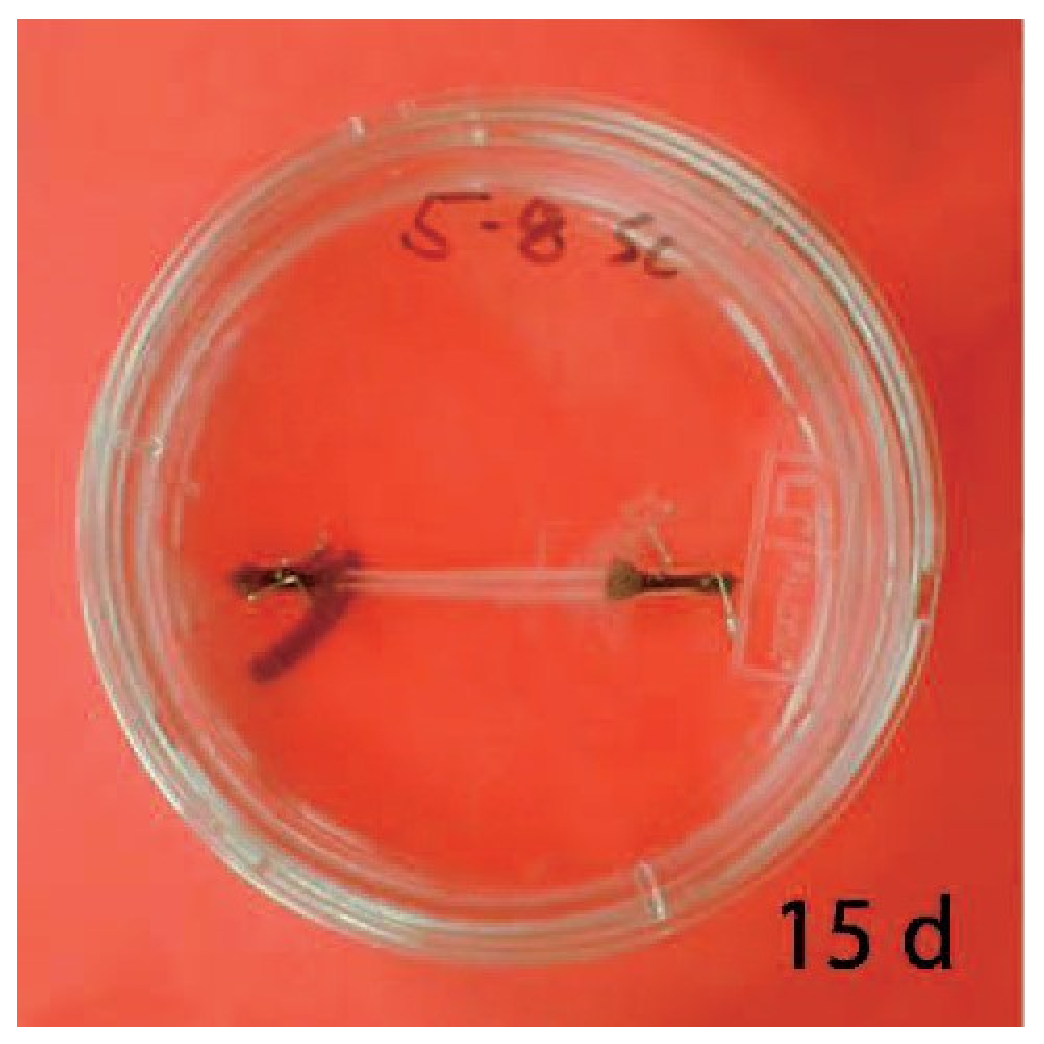
\includegraphics[width=10.00cm]{images/one-construct.eps}
\caption{Engineered tendon constructs. See \citet{Calve:04} for
  details.} 
\label{engconst}
\end{figure}

\begin{figure}[ht]
  \centering
  \psfrag{D}{\small$1.1284$ mm}
  \psfrag{H}{\small$12.0$ mm}
  {\includegraphics[width=5cm]{images/mesh.eps}}
  \caption{The finite element mesh used in the computations.}
  \label{egmesh}
\end{figure}

The theory presented in the preceding sections results in a system of
non-linear, coupled partial differential equations. A finite element
formulation employing a staggered scheme based upon operator splits
\cite{Armero-poroplasticity:99,Garikipatiox2:01} has been implemented
in {\tt FEAP} \citep{feapmanual} to solve the coupled problem. As an
example, in the biphasic problem involving solid and fluid
phases only, the basic solution scheme involves keeping the displacement
field fixed while solving for the concentration fields using the mass
transport equations. The resulting concentration fields are then fixed
to solve the mechanics problem. This procedure is repeated until the
resulting fields satisfy the differential equations within a specified
numerical tolerance.

The following examples aim to demonstrate the mathematical formulation
and aspects of the coupled phenomena as the tissue grows. The model
geometry, based on our engineered tendon constructs (see
Figure~\ref{engconst} and \citet{Calve:04}), is a cylinder 12 mm in length and 1 mm$^2$ in
cross-sectional area. The corresponding finite element mesh using
hexahedral elements, is shown in Figure~\ref{egmesh}.

The following numerical examples involve solution of a common set of
partial differential equations. The constutive models, however, vary as we
demonstrate the behaviour engendered by the many modelling
assumptions discussed in the paper. The balance of linear momentum
that we solve is (\ref{linearmombalance}) summed for $\iota =
\mathrm{c,f}$, with the constraint in (\ref{qrelation}) imposed. The
absence of significant acceleration in the problems under 
consideration allows us to solve the balance of linear momentum   
quasi-statically. The fluid mass balance equation is solved in the current
configuration, i.e. (\ref{massbalcurr}) for $\iota = \mathrm{f}$, but 
mass balance for the solid collagenous phase is solved in the
reference configuration, i.e. (\ref{massbalance1}) for $\iota =
\mathrm{c}$.  Mass balance for the solute is also solved in the
current configuration, but using the stabilized scheme in weak
form (\ref{stabilizedmassbal}). The Backward 
Euler algorithm is used for all mass transport equations. The
constitutive relation for the solid collagen follows
(\ref{wlcmeq}). The constitutive relation for the fluid stress follows
(\ref{Pf}) with 
\begin{equation}
h(\rho^\mathrm{f}) =
\frac{1}{2}\kappa^\mathrm{f}\left(\frac{\rho_{0_\mathrm{ini}}^\mathrm{f}}{\rho^\mathrm{f}}
- 1\right)^2,
\end{equation}

\noindent where $\kappa^\mathrm{f}$ is the fluid bulk modulus. The
tissue is modelled as being fluid saturated in $\Omega_t$ at $t = 0$,
i.e. (\ref{saturation}$_1$) holds with
$\rho^\mathrm{f}_{0_\mathrm{sat}} =
\rho^\mathrm{f}_{0_\mathrm{ini}}$. However, the tissue is allowed to 
become unsaturated in $\Omega_t$ for $t > 0$ due to void formation. Then,
the conditions set out in (\ref{cavitation})
apply. The chemical potential is then given by
(\ref{fickeanmobility}). The numerical examples that follow discuss further
specialization of the constitutive relations to other cases discussed
in the preceding sections. The numerical values of parameters\footnote{The
  mobility tensor reported in Table~\ref{parameters} is an
  order-of-magnitude estimate 
  recalculated from \citet{Hanetal:2000} to correspond to the 
  mobility used in this paper. These authors reported a mean value of
  $0.927\times 10^{-14}$ s, with a range of $1.14\times
  10^{-14}--0.58\times 10^{-14}$ s in terms of the mobility used
  here. Theirs is the mobility parallel to the fiber direction in
  Rabbit Achilles tendon. Our usage of it is as an isotropic
  mobility. Using anisotropic mobilities, or different values from the
  reported range changes the result
  quantitatively, but not qualitatively.}  that
have been used appear in Table \ref{parameters}.


Non-linear projection methods \citep{simotaylorpister:85} are used to treat the
near-incompressibility imposed by the fluid. Mixed methods, as described
in \cite{Garikipatiox2:01}, are used for stress (and strain) gradient
driven fluxes.

The initial and boundary
conditions have been chosen in order to model a few common mechanical and
chemical interventions on engineered tissue. However, we will not
attempt detailed descriptions of experiments, choosing to focus
instead on results that can be directly related to the models. A more
detailed comparison with experiments is forthcoming in a separate
communication. 

\subsection{A multiphasic problem based on enzyme-kinetics}
\label{enzyme_kinetics_eg}

\begin{table}
\centering
\begin{tabular}{lll}
\hline
\multicolumn{1}{c}{Parameter (Symbol)} & Value & Units\\
\hline
Chain density ($N$) & $7\times 10^{21}$ & $\mathrm{m}^{-3}$\\
Temperature ($\theta$)  & $310.6$ & K\\
Persistence length ($A$) & $2.10$ & --\\
Fully-stretched length ($L$) & $2.125$ & --\\
Unit cell axes ($a,\;b,\;c$) & $1.95,\;1.95,\;2.43$ & --\\
Bulk compressibility factors ($\gamma,\;\beta$) & $1000,\; 4.5$ & --\\
Fluid bulk modulus ($\kappa^f$) & $1$ & GPa\\
Fluid mobility tensor ($D^\mathrm{f}_{ij} = D^\mathrm{f}\delta_{ij}$) & $1\times 10^{-14}$
&s\\
%Fluid mol. wt. ($\sM^\mathrm{f}$)& $2.991\times 10^{-26}$ & $\mathrm{kg}$\\ 
Fibroblast concentration ($\rho_{\mathrm{cell}}$) & 0.2 &
kg.m$^{-3}$\\
Max. reaction rate ($k_{\mathrm{max}} = 5$) & 5 & s$^{-1}$\\
Max. solute concentration ($\rho^{\mathrm{s}}_m$) & 0.2 &
kg.m$^{-3}$\\
Solute diffusivity ($\bD^\mathrm{s}$) & $1\times 10^{-9}$ &  m$^{-2}$s\\
\hline
\end{tabular}
\caption{Material parameters used in the analysis.}
\label{parameters}
\end{table}

This first example can be viewed as a model for localised, bolus
delivery of regulatory chemicals to the tendon while accounting for
mechanical (stress) effects. A single solute species\footnote{Here, we
  envision the solute to be a protein playing 
  an essential role in growth by catalysing underlying biochemical
  reactions. An important example of this is a family of proteins,
  TGF$\beta$, which is a multi-functional peptide that controls numerous
  functions of many cell types \citep{Alberts:02}.} is considered,
denoted by s, and 
a uniform distribution of fibroblasts that are characterised by their
cell concentration, $\rho_{\mathrm{cell}}$. Both, Fickean diffusion of
the solute, and stress gradient driven fluid flow are incorporated in this
illustration. We use 
Michaelis-Menten enzyme kinetics [Equation~(\ref{enzymekineticseq})]
to determine the rates of solute consumption and collagen production
as a function of solute concentration. This non-linear relationship for
our choice of parameters is visualised in
Figure~\ref{eg3menten}. Here, the fluid phase does not  take part in
reactions, and hence $\Pi^\mathrm{f}=0$. 

\begin{figure}
\centering
\includegraphics[angle=270,width=10.00cm]{images/enzyme-kinetics.eps}
\caption{Variation of the collagen source term (kg.m$^{-3}$.s$^{-1}$)
  with solute concentration (kg.m$^{-3}$).}
\label{eg3menten}
\end{figure}

The tendon immersed in the bath is subjected to a constrictive
radial load, such
as would be imposed upon  manipulating it with a set of tweezers, as depicted in
Figure~\ref{constrictload}. The
maximum strain in the radial 
direction---experienced half-way through the height of the tendon---is
10\%. The applied strain in the radial direction decreases linearly
with distance from the central plane, and vanishes at the top and
bottom surfaces of the tendon. 


\begin{figure}[ht]
  \centering
  \psfrag{M}{\small $\bN\cdot\bM^f$}
  \psfrag{P}{\small ${\tiny\quad }~\bu$}
         {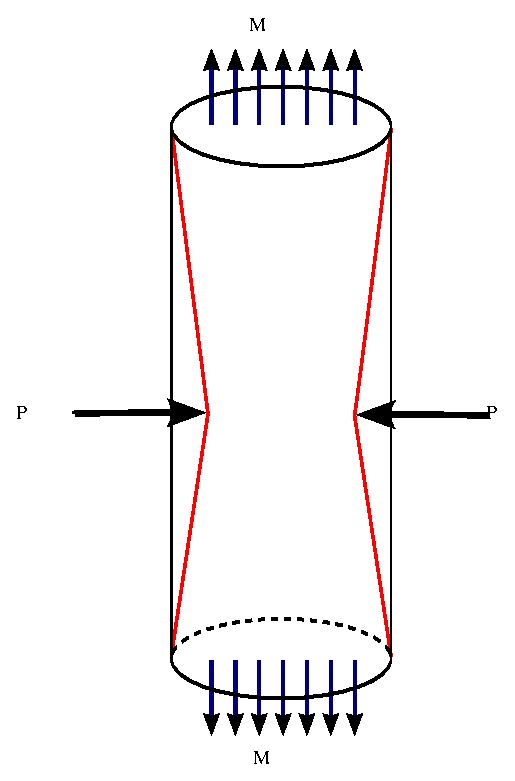
\includegraphics[width=5.0cm]{images/cylinder-in-bath.eps}}
	 \caption{Constrictive load applied to tendon immersed in a
	 bath.} 
	 \label{constrictload}
\end{figure}

The 
initial collagen concentration and the initial fluid concentration are
both 500~kg.m$^{-3}$ at every point in the tendon, and the fluid
concentration in the bath is 500~kg.m$^{-3}$. In
addition, a solute-rich bulb of radius 0.15~mm is introduced with
its centre on the axis of the tendon and situated 3~mm below the upper
circular face of the tendon. The initial solute concentration is
0.05~kg.m$^{-3}$ at all other points in the tendon, and increases
linearly with decreasing radius in this bulb to 1~kg.m$^{-3}$ at its
centre (see Figure~\ref{eg3ini}). The
parameters used are listed in Table~\ref{parameters}, and are relevant
to tendons.

\begin{figure}
\centering
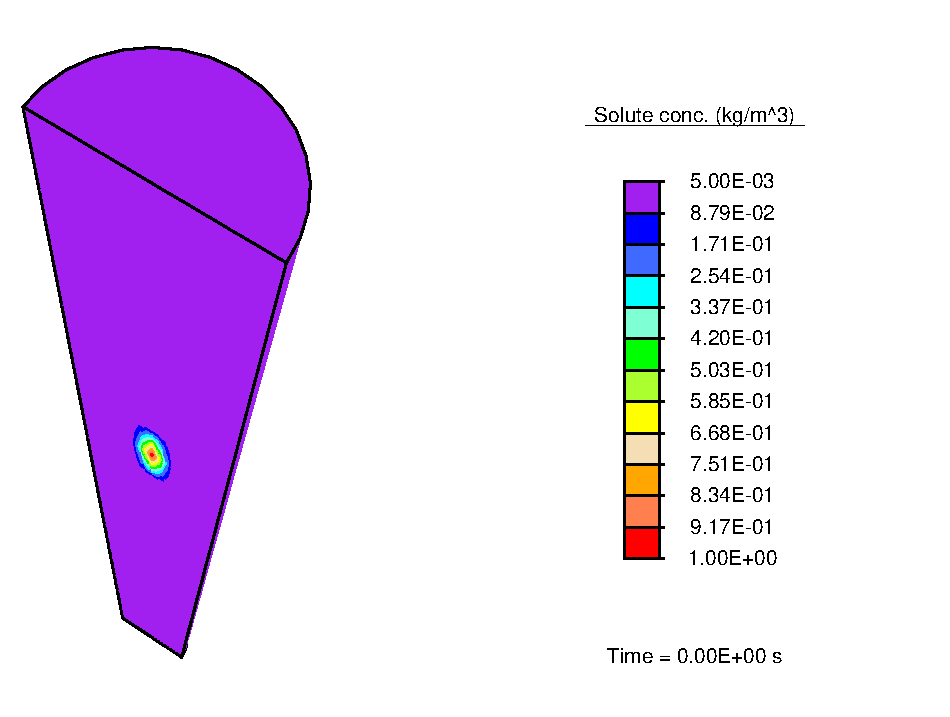
\includegraphics[width=10.00cm]{images/initial-solute-concentration.eps}
\caption{The solute concentration (kg.m$^{-3}$) initially.}
\label{eg3ini}
\end{figure}

The aim of this example is to compare the influences upon solute
transport from two mechanisms: Fluid stress gradient-driven transport,
arising from the applied constrictive load, and solute concentration
gradient-driven transport. These mechanisms have both been implicated
in nutrient supply to cells in soft tissue. The results of this
numerical example demonstrate that because the magnitude of the fluid mobility
for stress gradient driven transport is orders of magnitude
smaller than the diffusion coefficient for the solute through the
fluid, there is relatively only a small stress gradient driven flux,
and the transport of the solute is diffusion dominated. As a result,
the solute diffuses locally, but displays no
observable advection along the fluid. As the diffusion-driven solute
concentration in a region increases, the enzyme-kinetics model
results in a small source term for collagen production, and we observe nominal
growth. Figure~\ref{eg3conc} shows the collagen concentration at an
early time, $t=5\times10^{-2}$~s.

\begin{figure}
\centering
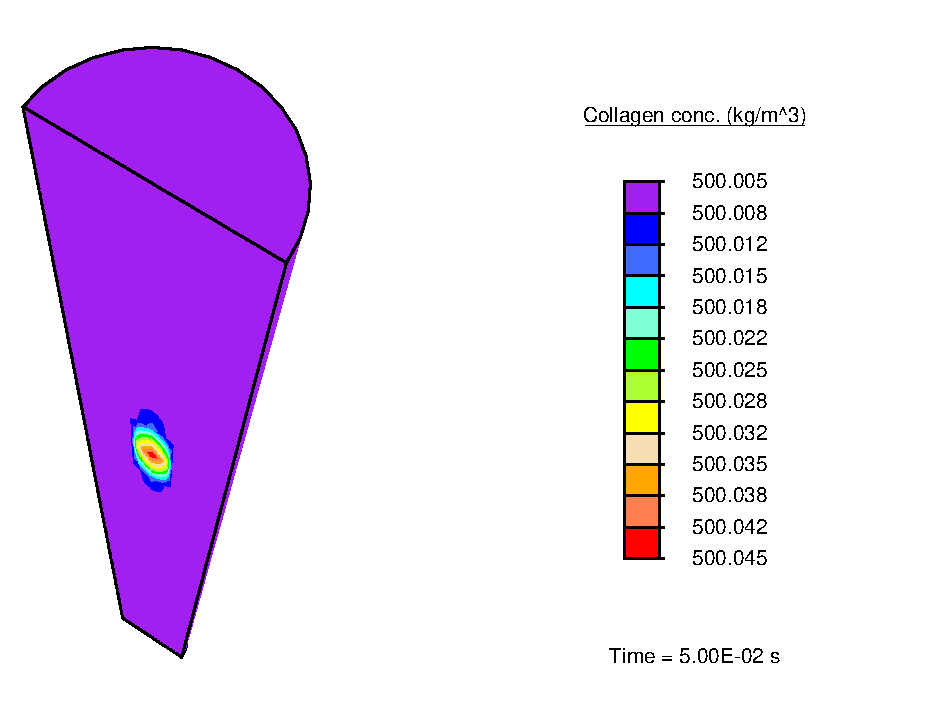
\includegraphics[width=10.00cm]{images/final-collagen-concentration.eps}
\caption{The collagen concentration (kg.m$^{-3}$) at time
  $t=5\times10^{-2}$~s.}
\label{eg3conc}
\end{figure}

This example incorporates all of the theory discussed in the
paper. However, it is a valuable exercise in
modelling to simplify the boundary value problem, and supress some of
the coupled phenomena in order to gain a better understanding of some
effcts. This is the approach followed in the next two numerical
examples. The detailed transport and mechanics induced by the
constrictive radial load are discussed first in Section~\ref{pinching}. 

\subsection{Examples exploring the biphasic nature of porous soft tissue}
\label{firstorder}

In these calculations, only two phases---fluid and collagen---are
included for the mass transport and mechanics. The parameters used in the analysis
are presented in Table~\ref{parameters}. 

%The mixing entropy of fluid in the mixture with collagen is
%written as $\eta_{\mathrm{mix}}^{f} = -\frac{k}{\sM^\mathrm{f}}
%\mathrm{log} (\frac{\rho^\mathrm{f}} {\rho})$, where
%$\sM^\mathrm{f}$ is the molecular weight of the fluid.

\subsubsection{The tendon under constriction}
\label{pinching}


In this example, the tendon immersed in a bath is subjected to the same
constrictive radial load as in Section~\ref{enzyme_kinetics_eg}. Since
that example demonstrated an insignificant amount of local collagen production
over this time scale, we have simplified the
problem by setting the source term $\Pi^\mathrm{c} = 0$. The total
duration of the simulation is 
10~s, and the radial strain is applied as a displacement boundary
condition, increasing linearly from no strain initially to the maximum
strain at time $t = 1~\mathrm{s}$. Again,
both the initial collagen 
concentration and the initial fluid concentration are 500~kg.m$^{-3}$
at every point in the tendon. This tendon is exposed to a bath where
the fluid concentration is 500~kg.m$^{-3}$.

While solving the balance of momentum for the biphasic problem
of the solid collagen and a fluid phase, we currently treat the
tissue as a single entity and employ a summation of
Equation~(\ref{linearmombalance}) over both species. Additionally,
condition~(\ref{qrelation}) allows us to avoid constitutive
prescription of the momentum transfer terms between solid collagen and
fluid phases,
$\bq^\mathrm{c}$ and $\bq^\mathrm{f}$. This facilitates considerable
simplification of the 
problem, but such a treatment requires additional assumptions on the
detailed deformation of the constitutive phases of the tissue. An
explicit assumption we have drawn on thus far is the equality of
the deformation gradient of the solid collagen and pore spaces,
allowing us to use the deformation gradient
$\bF$, suitably decomposed to account for change in fluid
concentration, to model the fluid stress. This assumption and its 
consequences have been discussed in Sections \ref{bomass},
\ref{growthkinem}, \ref{satswel}, \ref{compfluid}, \ref{tensionfluid}
and \ref{incompfluid}. Since the imposition of a common deformation gradient
results in an upper bound for the 
effective stiffness of the tissue and magnitudes of the fluxes
established, we refer to it as the {\em upper bound model}. This
assumption plays a fundamental role in determining the fluid flux driven
by the fluid stress gradient.

\begin{figure}[ht]
  \centering
      {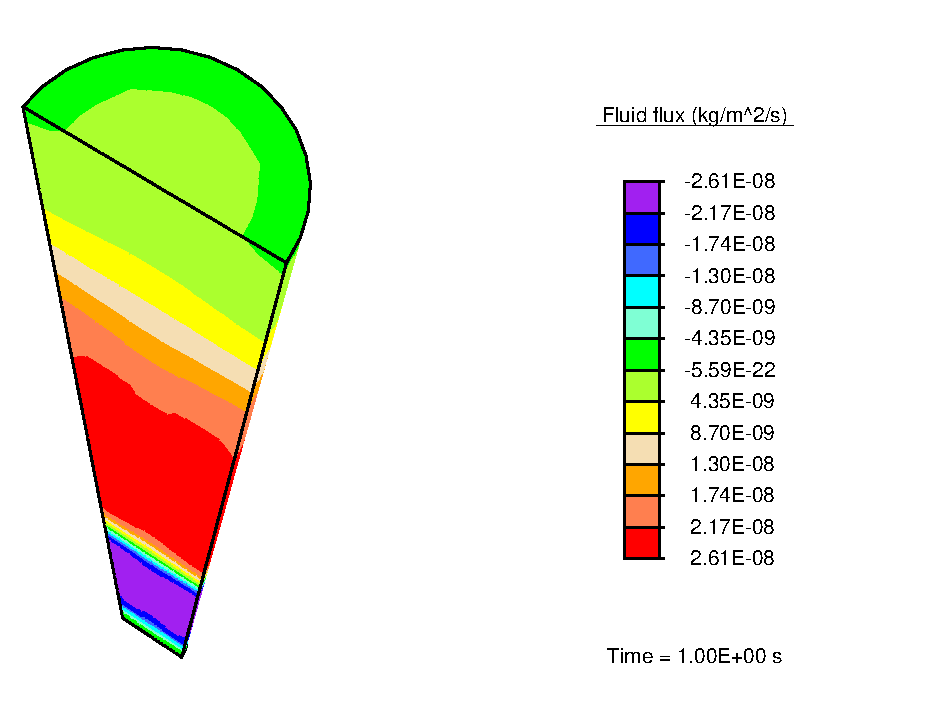
\includegraphics[width=10.00cm]{images/upper-bound-flux.eps}}
      \caption{{\em Upper bound} fluid flux (kg.m$^{-2}$.s$^{-1}$) in
        the vertical direction at time $t=1$~s.}
      \label{eg2flux}
\end{figure}

\noindent For this upper bound model, Figure~\ref{eg2flux} shows the fluid flux in
the vertical direction at the final stage of the constriction phase of
the simulation, i.e. at time $t=1$~s. The flux values are positive
above the central plane, forcing fluid upward, and negative below,
forcing fluid fluid downward. This stress-gradient induced fluid flux
results in a reference concentration distribution of the fluid that is
higher near the top and bottom faces, as seen in Figure~\ref{eg2conc}.

\begin{figure}[ht]
  \centering
      {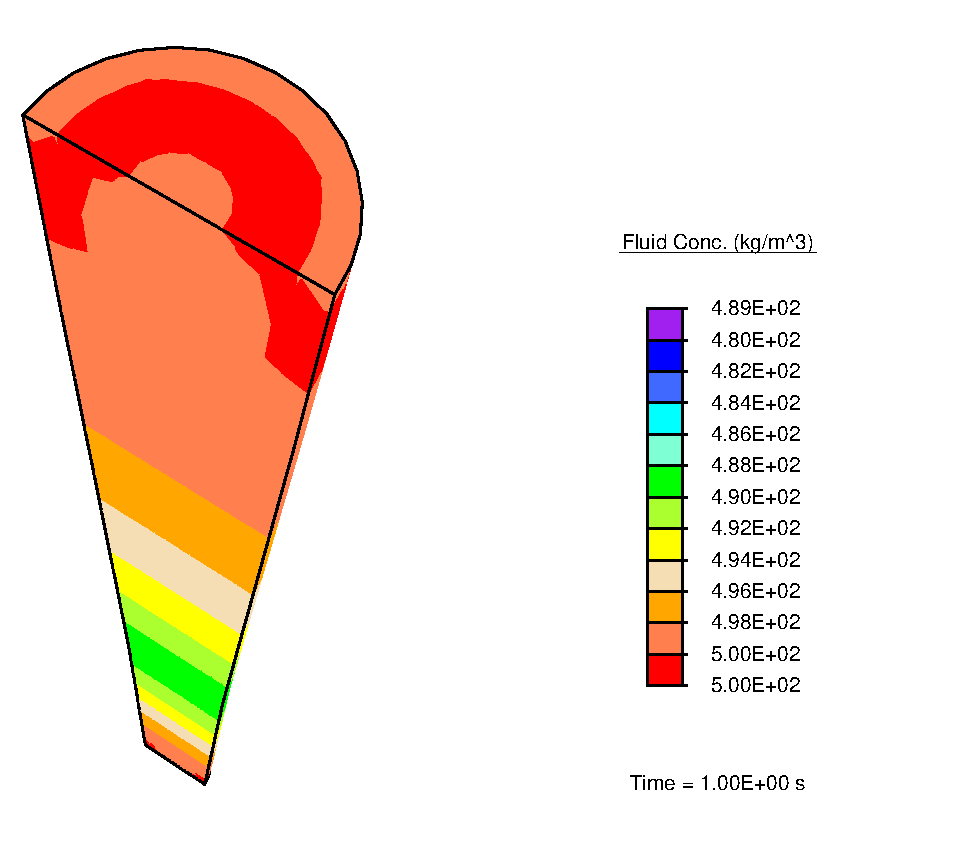
\includegraphics[width=10.00cm]{images/fluid-concentration.eps}}
      \caption{Reference fluid concentration (kg.m$^{-3}$) at time
      $t=1$~s.}
      \label{eg2conc}
\end{figure}

As a result, these regions would have seen a higher production of
collagen, or preferential growth, in the presence of non-zero source
terms. As discussed in Section~\ref{curr-ref-mb}, the mass transport
equations are solved in the current configuration, where physical
boundary conditions can be set directly. The values reported in
Figure~\ref{eg2conc} are pulled back from the current
configuration. The current concentrations do not change for this
boundary value problem. 

Solving a problem of this nature in the
reference configuration using $\rho_0^\mathrm{f} = $ const. as the
boundary condition to represent immersion of the tendon in a fluid bath
yields non-physical results, such as an unbounded flow. This occurs
since the imposed strain gradient causes a stress gradient in the
fluid that does not decay. The imposed boundary condition on $\rho_0^\mathrm{f}$
prevents a redistribution of concentration that would have provided an
opposing, internal gradient of stress, which in turn would drive the
flux to vanish.

The tendon is held fixed in the radial direction after the
constriction phase. The applied stress sets up a pressure wave in the
fluid travelling toward the top and bottom faces. As the fluid leaves
these surfaces, we observe that the tendon relaxes. This is seen in
Figure~\ref{topdisp}, which plots the vertical displacement of the top
face with time, showing a decrease in height of the tendon after the
constriction phase. We keep the centre of the bottom face of the
tendon fixed.

\begin{figure}[ht]
  \centering
      {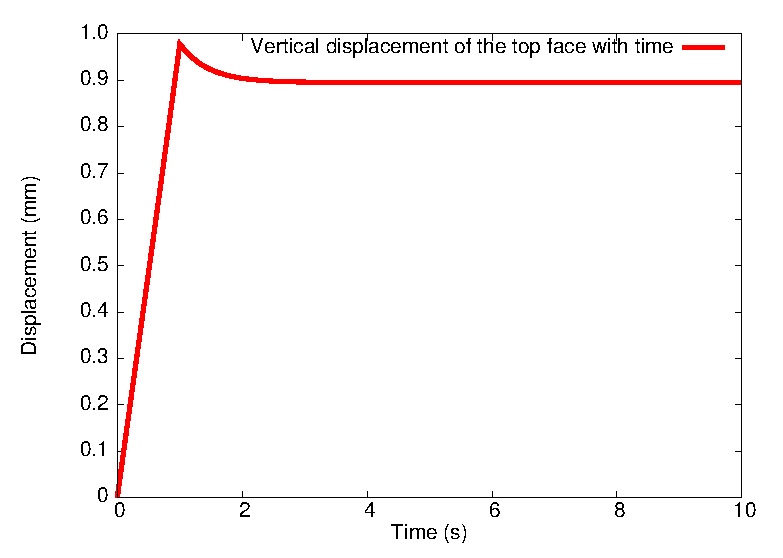
\includegraphics[width=10.00cm]{images/top-vertical-displacement.eps}}
      \caption{Relaxation of the top face of the tendon after the
      constriction phase.}
      \label{topdisp}
\end{figure}

In order to define a range of the magnitude of fluid flux, we now
introduce the {\em lower bound model} (on effective stiffness of the
tissue and, consequently, the magnitude of the fluid flux). For this lower bound, we
replace the earlier strain homogenisation requirement with a stress
homogenisation requirement, {\em viz.} equating the hydrostatic stress
of the solid phase and the fluid pressure in the current
configuration:

\begin{equation}
p^{\mathrm{f}}=\frac{1}{3} \mathrm{\small{tr}}[\Bsigma^{c}],
\label{equalpr}
\end{equation}

\noindent where $p^{\mathrm{f}}$ is the fluid pressure in the current
configuration, $\mbox{\small{tr}[\textbullet]}$ is the trace operator, and
$\Bsigma^{c}=\frac{1}{\mathrm{J^{c}}} \bP^{\mathrm{c}}
\bF^{\mathrm{c}^{\mathrm{T}}}$ is the Cauchy stress of the solid. The
Cauchy stress of an ideal fluid can be defined from its current
pressure as \mbox{$\Bsigma^{f}= p^{\mathrm{f}} \bone$.}
Figure~{\ref{lowerbound}} reports the value of the vertical flux under
the lower bound modelling assumption, using boundary conditions identical to the
previous calculation at time $t=1$~s, the final stage of the
constriction phase of the simulation. 


\begin{figure}[ht]
  \centering
      {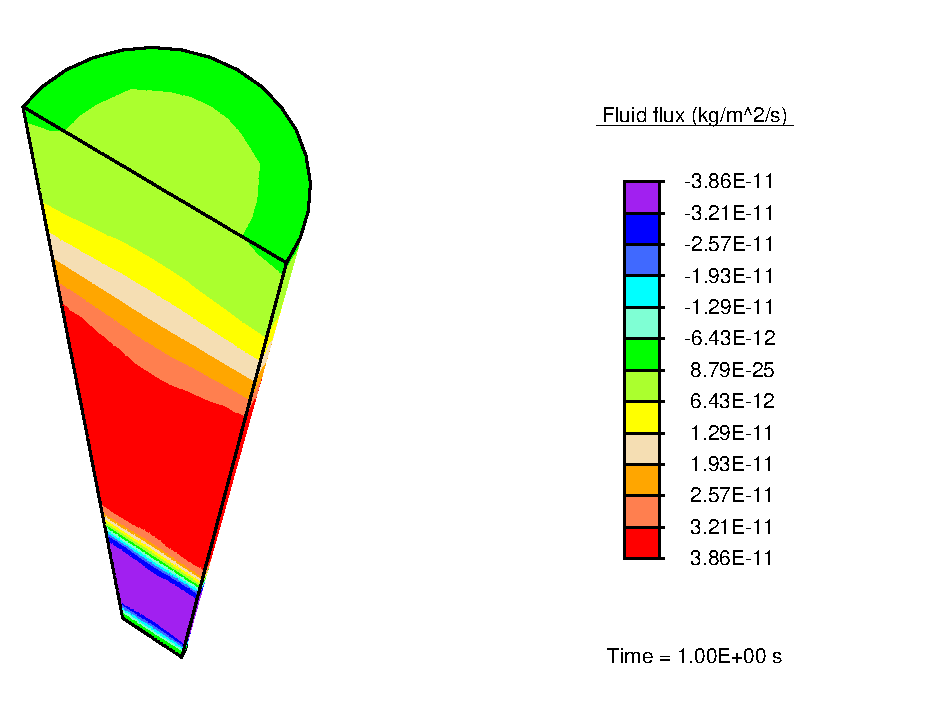
\includegraphics[width=10.00cm]{images/lower-bound-flux.eps}}
      \caption{{\em Lower bound} fluid flux (kg.m$^{-2}$.s$^{-1}$) in
        the vertical direction at time $t=1$~s.}
      \label{lowerbound}
\end{figure}

The fluid flux values reported in Figures~\ref{eg2flux} and
\ref{lowerbound} (corresponding to the upper and lower bound modelling
assumptions, respectively) are qualitatively similar, but differ by
about three orders of magnitude. This wide range points to the
importance of imposing the appropriate mechanical coupling model
between interacting phases. Note, however, that we have computed
bounds for the 
range of possible fluid flux values under the specified mechanical
loading. Recall, furthermore, that the example in Section
\ref{enzyme_kinetics_eg} used the upper bound model, and yet resulted
in no discernible advective solute transport. This suggests strongly
that, given the parameters in Table \ref{parameters}, convective
transport of nutrients in tendons is dominated by diffusive
transport. In future work, we will detail models that result in precise
field values for the fluxes, which will replace the upper and lower
bounds discussed here.  


This numerical example also points to the fact that a convenient
measure of the strength of 
coupling between the mechanics and mass transport equations is the
ratio of the variation in hydrostatic stress of the fluid to that of
the solid. In the lower bound case, where the fluid response is
defined by Equation~(\ref{equalpr}), it is instructive to note that
this ratio is unity. As a result, it is seen that the lower bound case
exhibits significantly weaker coupling than the upper bound case. In
the latter, variation in the common deformation gradient, $\delta
\bF$, causes instantaneous variation in \mbox{$\delta p^{\mathrm{f}} \approx
  O(\kappa^{\mathrm{f}} \delta \bF:\bF^{-\mathrm{T}})$} and in
\mbox{$\frac{1}{3} \delta\mathrm{\small{tr}}[\Bsigma^{c}] \approx
  O(\kappa^{\mathrm{c}} \delta \bF:\bF^{-\mathrm{T}})$}, where
$\kappa^{\mathrm{c}}$ is the bulk modulus of the solid. The ratio
$\frac{\delta p^{\mathrm{f}}}{\frac{1}{3} \delta
  \mathrm{\small{tr}}[\Bsigma^{c}]}$ is therefore \mbox{$\approx
O(\kappa^{\mathrm{f}}/\kappa^{\mathrm{c}}) \gg 1$}.

The strength of coupling between the equations plays a principal role
in the rate of convergence of the solution, as observed in
Table~\ref{resnorms}, where the residual norms of the equilibrium
equation (and
corresponding CPU times in seconds for an Intel\textregistered Xeon
3.4 GHz machine) are reported for the first 8 iterations of each of
the two cases. Recall that the staggered scheme involves solution of
the mechanics equation 
keeping the concentrations fixed, and the mass transport equation
keeping the displacements fixed, in turn, until the solution
converges. The table does not report the value of the residual norms
arising from the solution of the mass transport equation for the
fluid, which occurs after each reported solve of the of the mechanics
equation. Although the initial mechanics residual norms in successive
passes are decreasing linearly in both cases, the rapid decrease in
this quantity in
the weakly-coupled case ensures convergence in far fewer iterations
than the strongly coupled case. Thus, the corresponding CPU times
reported are also lower for the weakly coupled case. This is
advantageous. In addition to being more physical, as argued at
the beginning of Section \ref{swelling} immediately below, the lower
bound, weakly-coupled case makes it feasible to drive 
problems to longer, physiologically-relevant time-scales through the use
of larger time steps.

\begin{table}
\centering
\begin{tabular}{|r|c|c|c|c|}
  \hline
  Pass & \multicolumn{2}{c|}{Strongly coupled} &
         \multicolumn{2}{c|}{Weakly coupled}\\
  \cline{2-5} & Residual & CPU (s) & Residual & CPU (s)\\
  \hline\hline 
1     & $ 2.138\times 10^{-02}$ &   29.16   & $6.761 \times 10^{-04}$  &    28.5 \\
      & $ 3.093\times 10^{-04}$ &   55.85   & $1.075 \times 10^{-04}$  &    55.1 \\
      & $ 2.443\times 10^{-06}$ &   82.37   & $4.984 \times 10^{-06}$  &    81.8 \\
      & $ 2.456\times 10^{-08}$ &  109.61   & $1.698 \times 10^{-08}$  &   107.9 \\
      & $ 4.697\times 10^{-14}$ &  135.83   & $3.401 \times 10^{-13}$  &   134.1 \\
      & $ 1.750\times 10^{-16}$ &  163.18   & $1.1523\times 10^{-17}$  &   161.1 \\
\hline                                    
2     & $ 5.308\times 10^{-06}$ &  166.79   & $5.971 \times 10^{-08}$  &  192.5  \\
      & $ 4.038\times 10^{-10}$ &  193.36   & $4.285 \times 10^{-11}$  &  218.6  \\
      & $ 1.440\times 10^{-14}$ &  220.45   & $2.673 \times 10^{-15}$  &  246.1  \\
      & $ 4.221\times 10^{-17}$ &  247.04   & $                    $   &  \\
\hline                                    
3     & $ 5.186\times 10^{-06}$ &  250.62   & $2.194 \times 10^{-09}$  &  277.3  \\
      & $ 3.852\times 10^{-10}$ &  277.44   & $2.196 \times 10^{-13}$  &  304.2   \\
      & $ 1.369\times 10^{-14}$ &  304.16   & $1.096 \times 10^{-17}$  &  331.6   \\
      & $ 4.120\times 10^{-17}$ &  331.47   & $                    $   &  \\
\hline                                    
4     & $ 5.065\times 10^{-06}$ &  335.16   & $8.160 \times 10^{-11}$  &  363.2 \\ 
      & $ 3.674\times 10^{-10}$ &  362.24   & $7.923 \times 10^{-15}$  &  390.2 \\
      & $ 1.300\times 10^{-14}$ &  388.79   & $                    $   &  \\
      & $ 4.021\times 10^{-17}$ &  416.08   & $                    $   &  \\
\hline                                    
5     & $ 4.948\times 10^{-06}$ &  419.59   & $3.078 \times 10^{-12}$  &  421.4 \\
      & $ 3.503\times 10^{-10}$ &  446.24   & $3.042 \times 10^{-16}$  &  448.6 \\
      & $ 1.236\times 10^{-14}$ &  473.20   & $                    $   &  \\
      & $ 3.924\times 10^{-17}$ &  500.85   & $                    $   &  \\
\hline                                    
6     & $ 4.832\times 10^{-06}$ &  504.65   & $1.179 \times 10^{-13}$  &  479.9 \\
      & $ 3.340\times 10^{-10}$ &  531.28   & $1.291 \times 10^{-17}$  &  507.0 \\
      & $ 1.174\times 10^{-14}$ &  558.17   & $                    $   &  \\
      & $ 3.829\times 10^{-17}$ &  585.27   & $                    $   &  \\
\hline                                    
7     & $ 4.720\times 10^{-06}$ &  589.01   & $4.592 \times 10^{-15}$  &  537.8 \\
      & $ 3.184\times 10^{-10}$ &  616.24   & $5.152 \times 10^{-18}$  &  564.6 \\
      & $ 1.116\times 10^{-14}$ &  643.29   & $                    $   &  \\
      & $ 3.737\times 10^{-17}$ &  670.83   & $                    $   &  \\
\hline                                    
8     & $ 4.609\times 10^{-06}$ &  674.46   & $1.816 \times 10^{-16}$  &  595.5  \\
      & $ 3.034\times 10^{-10}$ &  701.74   & $5.040 \times 10^{-18}$  &  622.3  \\
      & $ 1.060\times 10^{-14}$ &  727.74   & $                    $   &  \\
      & $ 3.646\times 10^{-17}$ &  755.58   & $                    $   &  \\
\hline
\end{tabular}
\caption{Mechanics equation residual norms and corresponding CPU times
  in seconds for the first 8 passes of each of the two cases for a
  typical time increment, $\Delta t=$ 0.1 s.}
\label{resnorms}
\end{table}

\subsubsection{A swelling problem}
\label{swelling}

\begin{figure}[ht]
  \centering
     {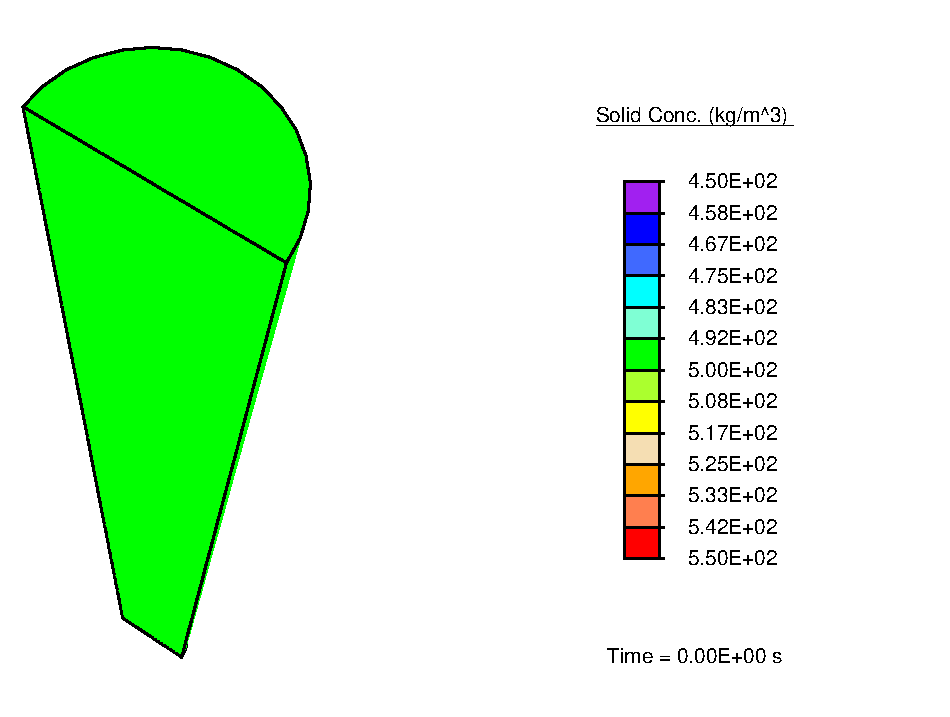
\includegraphics[width=10.00cm]{images/before-growth.eps}}
     \caption{The collagen initial concentration (kg.m$^{-3}$).}
     \label{before_growth}
\end{figure}

\begin{figure}[ht]
  \centering
     {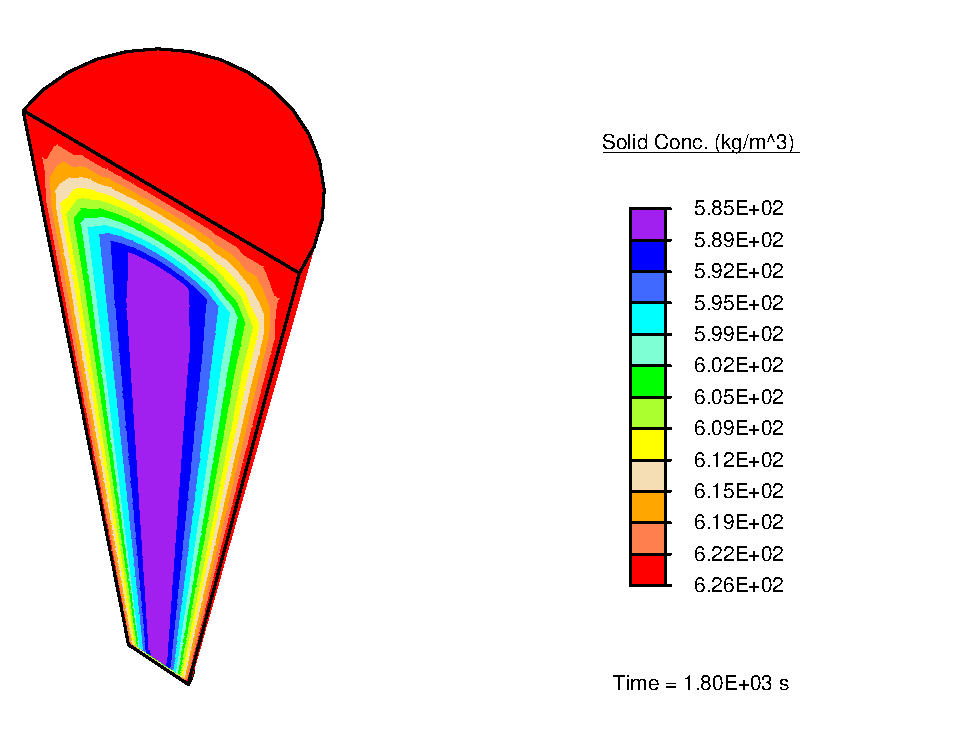
\includegraphics[width=10.00cm]{images/after-growth.eps}}
     \caption{The collagen concentration (kg.m$^{-3}$) after 1800~s.}
     \label{after_growth}
\end{figure}

\begin{figure}[ht]
  \centering
     {\includegraphics[angle=270,width=10.00cm]{images/stress-stretch.eps}}
     \caption{The stress (Pa) vs stretch curves before and after
       growth.}
     \label{stress_strain}
\end{figure}

\begin{figure}[ht]
  \centering
     {\includegraphics[angle=270,width=10.00cm]{images/volume-evolution-3.eps}}
     \caption{The volume of the tendon (m$^3$) evolving with
     time. Note the fluid transported-dominated regime until 25 s,
     followed by the longer reaction-dominated growth stage.}
     \label{volume_evolution}
\end{figure}

Motivated mainly by the recognition that the lower bound model for
solid-fluid mechanical coupling ensures convergence to a self-consistent
solution in just a few passes of the staggered solution scheme, we
adopt this version of the coupling for our final problem. On this
  note we point out that solution of the individual balances of linear
  momentum equation for the solid collagenous and fluid phases with
  the momentum transfer terms [$\bq^\mathrm{c}, \bq^\mathrm{f}$ in
  (\ref{linearmombalance})] is a
  statement of momentum balance between them. There is reason to
  suppose, therefore, that equating the solid collagen and fluid
  stress, or some component of these tensors as done in the lower
  bound model, is a reasonable approximation to explicitly solving the
  balance of linear momentum for each phase, including the momentum
  transfers. In contrast, equating the 
  deformation gradient of the solid collagen with deformation of the
  pore spaces subjects the fluid to a stress state also determined by
  this deformation gradient in the upper bound model. This
  approximation does not correspond to an underlying physical
  principle comparable to the satisfaction of individual
  balances of linear momentum for solid collagen and fluid, with
  momentum transfers. It is therefore somewhat less motivated and more
  questionable. Clearly, a rigorous analysis or numerical
  comparisons of all three models:
  upper bound, lower bound and direct solution of individual
  solid-fluid momentum balances, must be carried out to conclusively
  demonstrate this. It is a possible topic for a future paper.

In this example we will demonstrate the mechanical
effects of growth due to collagen production. In the interest of
focusing on this issue we assume that fibroblasts are
available, and that the fluid
phase bears the necessary nutrients for
collagen production dissolved at a suitable, constant
concentration. Collagen production is assumed to be governed by a
first-order rate 
law. Newly-produced collagen has proteoglycan molecules bound to it,
and they in turn bind water. We model this effect by associating a
loss of nutrient-bearing 
free fluid with collagen production. A fluid sink $\Pi^\mathrm{f}$ is
introduced following first order kinetics,

\begin{equation}
\Pi^\mathrm{f} = -k^\mathrm{f}(\rho_0^\mathrm{f}
- \rho_{0_\mathrm{ini}}^\mathrm{f}),
\end{equation}

\noindent as in \citet{growthpaper}. Here $k^\mathrm{f}$ is the
reaction rate, taken to be 0.07 $\mathrm{s}^{-1}$, and
$\rho_{0_\mathrm{ini}}^\mathrm{f}$ is the initial 
concentration of fluid. The collagen
source is mathemaically equivalent to the fluid sink: $\Pi^\mathrm{c} =
-\Pi^\mathrm{f}$. When $\rho_{0}^\mathrm{f} >
\rho_{0_\mathrm{ini}}^\mathrm{f}$, collagen is produced.

The boundary conditions in this example correspond to immersion of the
tendon in a nutrient-rich bath. The initial collagen concentration is
500~kg.m$^{-3}$ and the fluid concentration is 400~kg.m$^{-3}$ at
every point in the tendon. When this tendon is exposed to a bath
where the fluid concentration is 410~kg.m$^{-3}$,
i.e. $\rho^\mathrm{f}(\bx,t)=410~\mathrm{kg.m}^{-3} \forall \bx \in
\partial\Omega_t$, nutrient-rich fluid is transported into the tissue,
due to the pressure difference, induced by the concentration
difference, between the fluid in the tendon and in 
the bath (fluid stress gradient-driven flux). Thereby, the nutrient
concentration is elevated, leading to collagen production, fluid
consumption and, eventually, growth due to additional collagen. 

Figure~\ref{before_growth} shows the initial collagen concentration in
the tendon. After it has been immersed in the nutrient-rich bath for
1800~s, the tendon shows growth and the collagen concentration is
higher as seen in Figure~\ref{after_growth}. On performing a
uniaxial tension test on the tendon before and after growth, it is
observed (Figure~\ref{stress_strain}) that the grown tissue is stiffer
and stronger due to its higher collagen concentration. Also note that
there is a rapid, fluid transport-dominated swelling 
of the tendon  between 0 and 25 s 
following immersion in the fluid bath
(Figure~\ref{volume_evolution}). This causes a small volume change of 
$\approx 1.6$\%. In this transport-dominated regime the contribution
to tendon growth from collagen production is small. However, the
fluid-induced swelling saturates, and between
25 and 1800 s the reaction producing collagen dominates the growth
process, producing a further $\approx 6.8$\% volume change. Noting that the
range of collagen concentration in Figure~\ref{after_growth} is
$585-626\; \mbox{kg.m}^{-3}$, and that (\ref{isotropicgrowth}) gives $\bF^{\mathrm{g}^\mathrm{c}} = \left(
  \frac{\rho_0^\mathrm{c}}{\rho_{0_{\mathrm{ini}}}^\mathrm{c}}
  \right)^  {\frac{1}{3}} {\bf 1}$, this portion of the volume change
  is quite clearly due to collagen production. The total volume change
  of $8.4$\% corresponds to changes in each linear dimension of the
  tendon by only $\approx 2.7$\%, and is not discernible upon comparing
  Figures~\ref{before_growth} and \ref{after_growth}. It is, however,
  manifest in Figure~\ref{volume_evolution}.

\section{Conclusion}
\label{sec:5}

In this paper, we have discussed a number of enhancements to our
original growth formulation presented in \citet{growthpaper}. That
formulation has served as a platform for posing a very wide range of
questions on the biophysics of growth. Some issues, such as
saturation, incompressibility of the fluid species and its influence
upon the tissue response, and the roles of biochemical and strain
energy-dependent source terms are specific to soft biological
tissues. We note, however, that other issues are also applicable to a
number of systems with a porous solid, transported fluid and reacting
solutes. Included in these are issues of current versus reference
configurations for mass transport, swelling, Fickean diffusion, fluid
response in compression and tension, cavitation and the strength of
solid-fluid coupling..

These issues have been resolved using arguments posed easily in the
framework derived in \citet{growthpaper}. The interactions engendered
in the coupled reaction-trans\-port-mechanics system are complex, as
borne out by the numerical examples in
Section~\ref{numericalimplementation}. We are currently examining
combinations of sources defined in Section~\ref{sources}, and aim to
calibrate our choices from tendon growth experiments. The treatment of
these issues has led to a formulation more suited to the biophysics of
growing soft tissue, making progress toward our broader goal of
applying it to the study of wound healing, pathological hypertrophy
and atrophy, as well as a study of drug efficacy and interaction.
